% Options for packages loaded elsewhere
\PassOptionsToPackage{unicode}{hyperref}
\PassOptionsToPackage{hyphens}{url}
%
\documentclass[
  10pt,
  letterpaper,
  DIV=11,
  numbers=noendperiod,
  twoside]{scrartcl}

\usepackage{amsmath,amssymb}
\usepackage{setspace}
\usepackage{iftex}
\ifPDFTeX
  \usepackage[T1]{fontenc}
  \usepackage[utf8]{inputenc}
  \usepackage{textcomp} % provide euro and other symbols
\else % if luatex or xetex
  \usepackage{unicode-math}
  \defaultfontfeatures{Scale=MatchLowercase}
  \defaultfontfeatures[\rmfamily]{Ligatures=TeX,Scale=1}
\fi
\usepackage{lmodern}
\ifPDFTeX\else  
    % xetex/luatex font selection
  \setmainfont[ItalicFont=EB Garamond Italic,BoldFont=EB Garamond
Bold]{EB Garamond Math}
  \setsansfont[]{Europa-Bold}
  \setmathfont[]{Garamond-Math}
\fi
% Use upquote if available, for straight quotes in verbatim environments
\IfFileExists{upquote.sty}{\usepackage{upquote}}{}
\IfFileExists{microtype.sty}{% use microtype if available
  \usepackage[]{microtype}
  \UseMicrotypeSet[protrusion]{basicmath} % disable protrusion for tt fonts
}{}
\usepackage{xcolor}
\usepackage[left=1in, right=1in, top=0.8in, bottom=0.8in,
paperheight=9.5in, paperwidth=6.5in, includemp=TRUE, marginparwidth=0in,
marginparsep=0in]{geometry}
\setlength{\emergencystretch}{3em} % prevent overfull lines
\setcounter{secnumdepth}{3}
% Make \paragraph and \subparagraph free-standing
\ifx\paragraph\undefined\else
  \let\oldparagraph\paragraph
  \renewcommand{\paragraph}[1]{\oldparagraph{#1}\mbox{}}
\fi
\ifx\subparagraph\undefined\else
  \let\oldsubparagraph\subparagraph
  \renewcommand{\subparagraph}[1]{\oldsubparagraph{#1}\mbox{}}
\fi


\providecommand{\tightlist}{%
  \setlength{\itemsep}{0pt}\setlength{\parskip}{0pt}}\usepackage{longtable,booktabs,array}
\usepackage{calc} % for calculating minipage widths
% Correct order of tables after \paragraph or \subparagraph
\usepackage{etoolbox}
\makeatletter
\patchcmd\longtable{\par}{\if@noskipsec\mbox{}\fi\par}{}{}
\makeatother
% Allow footnotes in longtable head/foot
\IfFileExists{footnotehyper.sty}{\usepackage{footnotehyper}}{\usepackage{footnote}}
\makesavenoteenv{longtable}
\usepackage{graphicx}
\makeatletter
\def\maxwidth{\ifdim\Gin@nat@width>\linewidth\linewidth\else\Gin@nat@width\fi}
\def\maxheight{\ifdim\Gin@nat@height>\textheight\textheight\else\Gin@nat@height\fi}
\makeatother
% Scale images if necessary, so that they will not overflow the page
% margins by default, and it is still possible to overwrite the defaults
% using explicit options in \includegraphics[width, height, ...]{}
\setkeys{Gin}{width=\maxwidth,height=\maxheight,keepaspectratio}
% Set default figure placement to htbp
\makeatletter
\def\fps@figure{htbp}
\makeatother

\setlength\heavyrulewidth{0ex}
\setlength\lightrulewidth{0ex}
\usepackage[automark]{scrlayer-scrpage}
\clearpairofpagestyles
\cehead{
  Brian Weatherson
  }
\cohead{
  Some Data about Citation Trends
  }
\ohead{\bfseries \pagemark}
\cfoot{}
\makeatletter
\newcommand*\NoIndentAfterEnv[1]{%
  \AfterEndEnvironment{#1}{\par\@afterindentfalse\@afterheading}}
\makeatother
\NoIndentAfterEnv{itemize}
\NoIndentAfterEnv{enumerate}
\NoIndentAfterEnv{description}
\NoIndentAfterEnv{quote}
\NoIndentAfterEnv{equation}
\NoIndentAfterEnv{longtable}
\NoIndentAfterEnv{abstract}
\renewenvironment{abstract}
 {\vspace{-1.25cm}
 \quotation\small\noindent\rule{\linewidth}{.5pt}\par\smallskip
 \noindent }
 {\par\noindent\rule{\linewidth}{.5pt}\endquotation}
\KOMAoption{captions}{tableheading}
\makeatletter
\@ifpackageloaded{caption}{}{\usepackage{caption}}
\AtBeginDocument{%
\ifdefined\contentsname
  \renewcommand*\contentsname{Table of contents}
\else
  \newcommand\contentsname{Table of contents}
\fi
\ifdefined\listfigurename
  \renewcommand*\listfigurename{List of Figures}
\else
  \newcommand\listfigurename{List of Figures}
\fi
\ifdefined\listtablename
  \renewcommand*\listtablename{List of Tables}
\else
  \newcommand\listtablename{List of Tables}
\fi
\ifdefined\figurename
  \renewcommand*\figurename{Figure}
\else
  \newcommand\figurename{Figure}
\fi
\ifdefined\tablename
  \renewcommand*\tablename{Table}
\else
  \newcommand\tablename{Table}
\fi
}
\@ifpackageloaded{float}{}{\usepackage{float}}
\floatstyle{ruled}
\@ifundefined{c@chapter}{\newfloat{codelisting}{h}{lop}}{\newfloat{codelisting}{h}{lop}[chapter]}
\floatname{codelisting}{Listing}
\newcommand*\listoflistings{\listof{codelisting}{List of Listings}}
\makeatother
\makeatletter
\makeatother
\makeatletter
\@ifpackageloaded{caption}{}{\usepackage{caption}}
\@ifpackageloaded{subcaption}{}{\usepackage{subcaption}}
\makeatother
\ifLuaTeX
  \usepackage{selnolig}  % disable illegal ligatures
\fi
\IfFileExists{bookmark.sty}{\usepackage{bookmark}}{\usepackage{hyperref}}
\IfFileExists{xurl.sty}{\usepackage{xurl}}{} % add URL line breaks if available
\urlstyle{same} % disable monospaced font for URLs
\hypersetup{
  pdftitle={Some Data about Citation Trends},
  pdfauthor={Brian Weatherson},
  hidelinks,
  pdfcreator={LaTeX via pandoc}}

\title{Some Data about Citation Trends}
\author{Brian Weatherson}
\date{2024}

\begin{document}
\maketitle
\begin{abstract}
In the future I plan to write something substantive about trends in
citations in philosophy journals. This is a presentation of some of the
underlying data, with some small remarks about the big picture trends.
(I earlier published a version of this that used data starting in 1976.
I've now added 20 years more data.)
\end{abstract}

\setstretch{1.1}
I recently downloaded citation data for 100 philosophy journals from Web
of Science. This note presents some of the data about trends in citation
patterns since 1956. My main interest here is in seeing which changes
there have been in what was cited over time, but there are lots of
interesting nuggets. Later I'll write a real paper actually going into
what some of the data mean, but for now I'm just presenting it for
public consumption.

\section{Methodology}\label{sec-methodology}

\subsection{The Articles Being Studied}\label{sec-articles-studied}

Via the University of Michigan, I got the latest available database for
Web of Science circa January 2024. I created a file of every citation
where both the citing article and the cited article were from one of the
100 journals in Table~\ref{tbl-list-of-journals}, in the years that they
were indexed by Web of Science.

\begin{longtable}[]{@{}
  >{\raggedright\arraybackslash}p{(\columnwidth - 6\tabcolsep) * \real{0.5747}}
  >{\raggedleft\arraybackslash}p{(\columnwidth - 6\tabcolsep) * \real{0.1034}}
  >{\raggedleft\arraybackslash}p{(\columnwidth - 6\tabcolsep) * \real{0.1264}}
  >{\raggedleft\arraybackslash}p{(\columnwidth - 6\tabcolsep) * \real{0.1954}}@{}}

\caption{\label{tbl-list-of-journals}The journals included in this
study}

\tabularnewline

\toprule\noalign{}
\begin{minipage}[b]{\linewidth}\raggedright
Journal
\end{minipage} & \begin{minipage}[b]{\linewidth}\raggedleft
Articles
\end{minipage} & \begin{minipage}[b]{\linewidth}\raggedleft
First Year
\end{minipage} & \begin{minipage}[b]{\linewidth}\raggedleft
Most Recent Year
\end{minipage} \\
\midrule\noalign{}
\endhead
\bottomrule\noalign{}
\endlastfoot
Acta Philosophica & 211 & 2009 & 2022 \\
American Philosophical Quarterly & 1755 & 1964 & 2021 \\
Analysis & 2615 & 1975 & 2022 \\
Analytic Philosophy & 169 & 2016 & 2022 \\
Archiv Fur Geschichte Der Philosophie & 676 & 1975 & 2022 \\
Australasian Journal Of Philosophy & 1683 & 1975 & 2022 \\
Biology \& Philosophy & 1117 & 1988 & 2022 \\
British Journal For The History Of Philosophy & 760 & 2007 & 2022 \\
British Journal For The Philosophy Of Science & 1499 & 1956 & 2022 \\
British Journal Of Aesthetics & 1369 & 1975 & 2022 \\
Bulletin Of Symbolic Logic & 81 & 2003 & 2022 \\
Canadian Journal Of Philosophy & 1497 & 1975 & 2022 \\
Croatian Journal Of Philosophy & 329 & 2007 & 2022 \\
Dialogue & 1464 & 1975 & 2022 \\
Economics And Philosophy & 116 & 2003 & 2022 \\
Episteme & 551 & 2005 & 2022 \\
Ergo & 213 & 2016 & 2021 \\
Erkenntnis & 1744 & 2000 & 2022 \\
Ethical Theory And Moral Practice & 854 & 2008 & 2022 \\
Ethics & 1564 & 1956 & 2022 \\
European Journal For Philosophy Of Science & 449 & 2011 & 2022 \\
European Journal Of Philosophy & 914 & 1998 & 2022 \\
Heythrop Journal & 792 & 1975 & 2014 \\
History And Philosophy Of Logic & 475 & 1992 & 2022 \\
Hume Studies & 111 & 2010 & 2022 \\
Hypatia & 607 & 2009 & 2022 \\
Inquiry & 1743 & 1966 & 2022 \\
International Journal For Philosophy Of Religion & 1098 & 1975 & 2022 \\
International Philosophical Quarterly & 1543 & 1961 & 2022 \\
Journal Of Aesthetics And Art Criticism & 1473 & 1975 & 2022 \\
Journal Of Applied Philosophy & 607 & 2006 & 2022 \\
Journal Of Chinese Philosophy & 1234 & 1973 & 2022 \\
Journal Of Consciousness Studies & 1356 & 2000 & 2022 \\
Journal Of Indian Philosophy & 1034 & 1975 & 2022 \\
Journal Of Medical Ethics & 270 & 1975 & 2022 \\
Journal Of Moral Philosophy & 347 & 2005 & 2022 \\
Journal Of Philosophical Logic & 1411 & 1972 & 2022 \\
Journal Of Philosophical Research & 508 & 2005 & 2022 \\
Journal Of Philosophy & 2706 & 1956 & 2022 \\
Journal Of Political Philosophy & 282 & 2003 & 2022 \\
Journal Of Social Philosophy & 481 & 2008 & 2022 \\
Journal Of Symbolic Logic & 192 & 1968 & 2022 \\
Journal Of The American Philosophical Association & 306 & 2015 & 2022 \\
Journal Of The History Of Ideas & 2101 & 1956 & 2022 \\
Journal Of The History Of Philosophy & 1083 & 1975 & 2022 \\
Journal Of The Philosophy Of History & 239 & 2010 & 2022 \\
Journal Of Value Inquiry & 1358 & 1980 & 2022 \\
Kant-Studien & 1068 & 1975 & 2022 \\
Kantian Review & 293 & 2010 & 2022 \\
Kennedy Institute Of Ethics Journal & 551 & 1995 & 2022 \\
Law And Philosophy & 208 & 2003 & 2022 \\
Logique Et Analyse & 339 & 2007 & 2021 \\
Metaphilosophy & 1470 & 1975 & 2022 \\
Midwest Studies In Philosophy & 107 & 1984 & 1988 \\
Mind & 1906 & 1956 & 2022 \\
Mind \& Language & 155 & 2003 & 2022 \\
Minds And Machines & 192 & 2003 & 2022 \\
Monist & 1911 & 1962 & 2022 \\
Notre Dame Journal Of Formal Logic & 424 & 2009 & 2022 \\
Noûs & 1443 & 1975 & 2022 \\
Pacific Philosophical Quarterly & 1190 & 1980 & 2022 \\
Philosophers' Imprint & 353 & 2010 & 2022 \\
Philosophia & 2050 & 1975 & 2022 \\
Philosophia Mathematica & 221 & 2008 & 2022 \\
Philosophical Explorations & 353 & 2008 & 2022 \\
Philosophical Forum & 802 & 1971 & 2022 \\
Philosophical Investigations & 676 & 1983 & 2022 \\
Philosophical Papers & 225 & 2009 & 2022 \\
Philosophical Perspectives & 275 & 2007 & 2022 \\
Philosophical Psychology & 291 & 2003 & 2022 \\
Philosophical Quarterly & 1341 & 1975 & 2022 \\
Philosophical Review & 988 & 1956 & 2022 \\
Philosophical Studies & 5210 & 1956 & 2022 \\
Philosophical Topics & 106 & 1981 & 1986 \\
Philosophy & 1951 & 1956 & 2022 \\
Philosophy \& Public Affairs & 698 & 1971 & 2022 \\
Philosophy And Phenomenological Research & 3149 & 1956 & 2022 \\
Philosophy And Rhetoric & 886 & 1975 & 2022 \\
Philosophy Compass & 540 & 2015 & 2022 \\
Philosophy East \& West & 1488 & 1966 & 2022 \\
Philosophy Of Science & 3020 & 1956 & 2022 \\
Philosophy Of The Social Sciences & 914 & 1975 & 2022 \\
Phronesis & 743 & 1975 & 2022 \\
Politics Philosophy \& Economics & 195 & 2008 & 2022 \\
Ratio & 1040 & 1974 & 2022 \\
Review Of Metaphysics & 1560 & 1956 & 2022 \\
Review Of Symbolic Logic & 535 & 2008 & 2022 \\
Russell & 379 & 1975 & 2022 \\
Social Philosophy \& Policy & 893 & 1983 & 2021 \\
South African Journal Of Philosophy & 726 & 1987 & 2022 \\
Southern Journal Of Philosophy & 1899 & 1976 & 2022 \\
Southwestern Journal Of Philosophy & 422 & 1970 & 1980 \\
Studia Logica & 666 & 2010 & 2022 \\
Studies In History And Philosophy Of Science & 1660 & 1974 & 2022 \\
Synthese & 6978 & 1966 & 2022 \\
Theoria & 395 & 2007 & 2022 \\
Thought & 188 & 2016 & 2021 \\
Topoi & 1113 & 1982 & 2022 \\
Transactions Of The Charles S Peirce Society & 1132 & 1975 & 2022 \\
Utilitas & 360 & 2009 & 2022 \\

\end{longtable}

Of course the first year isn't the first year the journal started
publishing; it's when Web of Science started indexing them. And the last
year isn't when they ceased publishing; it's the most recent year
indexed. Web of Science is very slow at adding journals, and at adding
volumes. But it is, as far as I've found, pretty accurate within what it
adds.

One big exception to this is that it's never really understood how to
handle the `supplements' to \emph{Noûs}, i.e., \emph{Philosophical
Perspectives} and \emph{Philosophical Issues}. Some of these are
recorded as being their own thing, some of them are recorded as special
issues of \emph{Noûs}. In the latter case, the citations often only
start being tracked several years after publication, and the
bibliographic information is spotty. I've manually removed the ones that
were listed as being published in \emph{Noûs} but actually in one of the
supplements, because the data didn't seem sufficiently reliable.

I've also manually added citations to articles published in
\emph{Journal of Philosophy} between 1971 and 1974. I don't have good
data for what was cited in those articles. I don't know why Web of
Science indexes the Journal before and after that period, but it's an
important gap. Several of the most important articles of the journals
era are published in the Journal in those years, so I felt it was
important to include them. I hope that the manual adding I did led to
values on the same scale as what I got from everything else, but this is
a possible source of noise in the data.

Because Web of Science keeps adding journals, and journals keep getting
larger, the number of articles in this study keeps going up. The only
downward pressure comes from the fact that some journals haven't been
indexed for 2022 or even, in some cases, 2021.
Figure~\ref{fig-number-of-articles-by-year} shows how many articles each
year are in the study.

\begin{figure}

\centering{

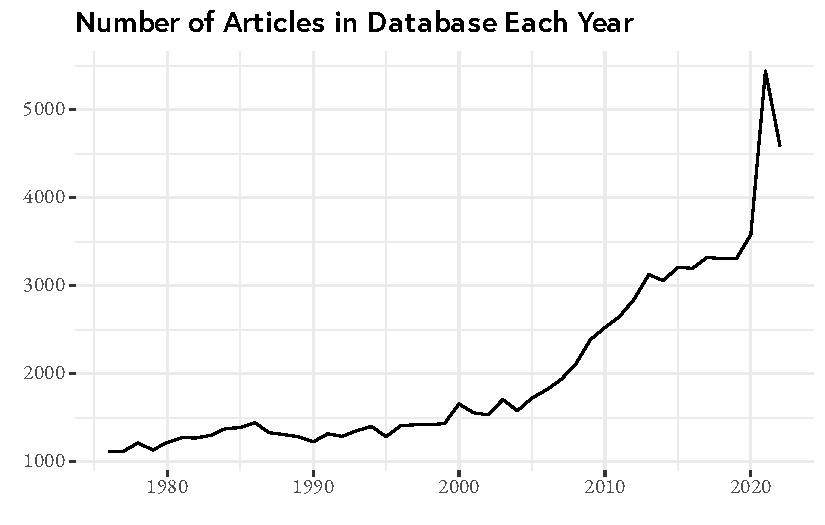
\includegraphics{citations_files/figure-pdf/fig-number-of-articles-by-year-1.pdf}

}

\caption{\label{fig-number-of-articles-by-year}Number of articles in the
study each year}

\end{figure}%

On top of that, citation practices have changed and people now cite much
more widely than they used to. So the number of citations recorded each
year (to articles since 1956 indexed in these 100 journals), has risen
rather dramatically, as shown in
Figure~\ref{fig-number-of-citations-by-year}.

\begin{figure}

\centering{

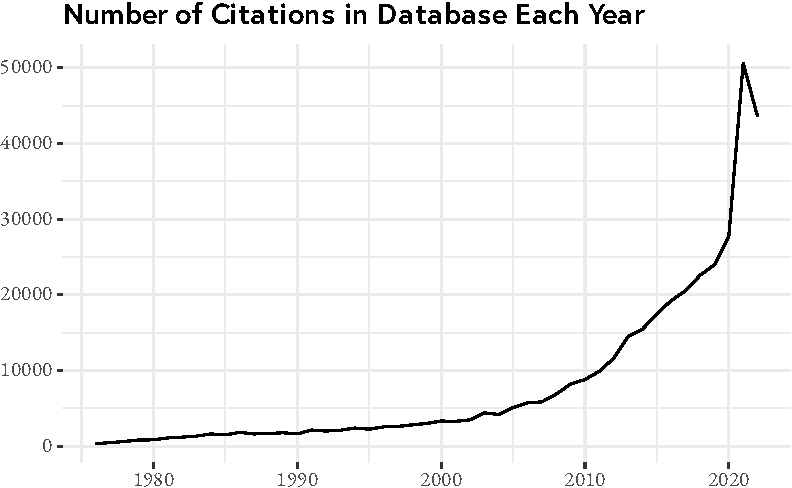
\includegraphics{citations_files/figure-pdf/fig-number-of-citations-by-year-1.pdf}

}

\caption{\label{fig-number-of-citations-by-year}Number of citations to
articles in the study each year}

\end{figure}%

On the other hand, since the overwhelming majority of citations are to
articles published earlier than the citing article, a larger number of
citations in total might be consistent with fewer citations per article
available to be cited. If we somewhat arbitrarily set the universe of
possible cited papers to be the set of papers with the same publication
date as the citing article or earlier,
Figure~\ref{fig-average-of-citations-by-year} shows how often the
average paper was cited each year (in these 100 journals).

\begin{figure}

\centering{

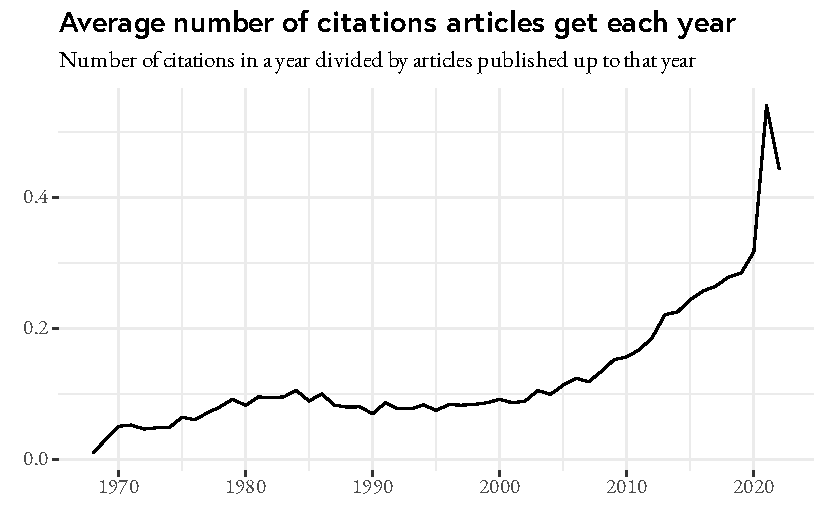
\includegraphics{citations_files/figure-pdf/fig-average-of-citations-by-year-1.pdf}

}

\caption{\label{fig-average-of-citations-by-year}Average number of
citations per available article in each each year}

\end{figure}%

Between about 1978 and 2004, the different forces are roughly balanced.
There are more papers, and each paper cites more often, but there are
more papers available to be cited, and the mean stays at about 0.1. (Of
course articles do get cited outside of journals indexed in Web of
Science, but it's still a bit humbling to realise that's the historical
average, even if one gets published in a journal as good as one of
these.) But then the forces pushing this number up take over. This is
important context for a lot of the graphs below, where the typical
article will have a graph of citations per year that looks a bit like
this.

\subsection{The Focus}\label{sec-focus}

For each year up to 2015, I made three lists. (After 2015 the citation
data is all too new to be particularly useful I think.) First, a list of
the articles published that year sorted by how many times they are
cited. Second, the same list sorted by how many times they are cited in
what I call \emph{early} years. That's either the first ten years after
publication, or half of the time between publication and 2022, whichever
is shorter. Third, the same list sorted by how many times they are cited
in what I call \emph{late} years, which is either the last ten years of
the study, or the years since publication that are not `early', again
whichever is shorter. Given how many of the citations come from the last
few years, the first and third lists overlap a lot. As we get closer to
the end of the study, the early cites tend to be very volatile, and
there is a bit of impact from how easy journals made it for their papers
to be cited prior to official publication through online early access.

After making those three lists, I found the largest \emph{n} such that
taking the top \emph{n} from those three lists gave me nine total
articles per year. (If forced to choose, I chose the articles with the
most total citations.) So we got a mix largely of highly cited articles,
and articles that were highly cited soon after publication. With nine
articles each year, and sixty years between 1976 and 2015, we should end
up with 540 articles.

Having built that list, I decided that articles with fewer than twenty
citations (in these 100 journals) were not cited often enough that it
made much sense to talk about trends in their citation pattern. So I
filtered the list down to only include articles with twenty or more
citations. The result is that we have 500 articles in total.

The 500 articles are, for better and for worse, a pretty representative
sample of what was happening in those journals, and in particular what
was being widely talked about in those journals. They wouldn't match up
with my list of the best 500 articles from those forty years, or I
suspect anyone else's list of the best 500 articles. But I do think they
are an interesting model of the field as it was across those years.

It was not a surprise that the famously high prestige journals have the
bulk of these articles. But there was more variation within the list
than some may have expected, as we see in
Table~\ref{tbl-journals-in-main-bib}.

\begin{longtable}[]{@{}lr@{}}

\caption{\label{tbl-journals-in-main-bib}Which journals the 500 articles
appeared in.}

\tabularnewline

\toprule\noalign{}
Journal & Articles \\
\midrule\noalign{}
\endhead
\bottomrule\noalign{}
\endlastfoot
Journal Of Philosophy & 96 \\
Philosophical Review & 72 \\
Philosophical Studies & 40 \\
Noûs & 36 \\
Philosophy Of Science & 29 \\
Mind & 27 \\
Philosophy And Phenomenological Research & 26 \\
American Philosophical Quarterly & 17 \\
Ethics & 17 \\
Philosophy \& Public Affairs & 16 \\
Journal Of Philosophical Logic & 12 \\
Philosophical Quarterly & 12 \\
Synthese & 12 \\
Australasian Journal Of Philosophy & 11 \\
Analysis & 10 \\
British Journal For The Philosophy Of Science & 10 \\
Monist & 9 \\
Philosophers' Imprint & 6 \\
Pacific Philosophical Quarterly & 5 \\
Biology \& Philosophy & 3 \\
Inquiry & 3 \\
Philosophical Perspectives & 3 \\
Philosophy & 3 \\
Canadian Journal Of Philosophy & 2 \\
Erkenntnis & 2 \\
Hypatia & 2 \\
Journal Of The American Philosophical Association & 2 \\
Midwest Studies In Philosophy & 2 \\
Ratio & 2 \\
Review Of Metaphysics & 2 \\
Studies In History And Philosophy Of Science & 2 \\
Analytic Philosophy & 1 \\
Episteme & 1 \\
Journal Of Consciousness Studies & 1 \\
Journal Of Political Philosophy & 1 \\
Metaphilosophy & 1 \\
Mind \& Language & 1 \\
Philosophia & 1 \\
Philosophical Psychology & 1 \\
Philosophy Compass & 1 \\

\end{longtable}

Around half the articles (257 out of 500) are in the journals widely
taken to be the big five: Journal of Philosophy, Philosophical Review,
Mind, Noûs, and Philosophy and Phenomenological Research.
Table~\ref{tbl-recent-journals-in-main-bib} shows what happens if we
restrict attention to just the last fifteens years, and look at which
articles from 2006 to 2020 are widely cited in this sense. The
percentage that are in these five journals falls slightly: it is now 54
out of 120. And the order at the top has changed a bit, as
Table~\ref{tbl-recent-journals-in-main-bib} shows.

\begin{longtable}[]{@{}lr@{}}

\caption{\label{tbl-recent-journals-in-main-bib}Which journals the most
recent 120 articles appeared in.}

\tabularnewline

\toprule\noalign{}
Journal & Articles \\
\midrule\noalign{}
\endhead
\bottomrule\noalign{}
\endlastfoot
Noûs & 20 \\
Philosophical Studies & 16 \\
Philosophy And Phenomenological Research & 11 \\
Journal Of Philosophy & 8 \\
Mind & 8 \\
Philosophical Review & 7 \\
Philosophers' Imprint & 6 \\
Synthese & 5 \\
Philosophical Quarterly & 4 \\
Inquiry & 3 \\
Journal Of Philosophical Logic & 3 \\
Philosophical Perspectives & 3 \\
Australasian Journal Of Philosophy & 2 \\
Biology \& Philosophy & 2 \\
British Journal For The Philosophy Of Science & 2 \\
Erkenntnis & 2 \\
Ethics & 2 \\
Hypatia & 2 \\
Journal Of The American Philosophical Association & 2 \\
Pacific Philosophical Quarterly & 2 \\
Philosophy Of Science & 2 \\
Analytic Philosophy & 1 \\
Episteme & 1 \\
Journal Of Consciousness Studies & 1 \\
Journal Of Political Philosophy & 1 \\
Mind \& Language & 1 \\
Monist & 1 \\
Philosophy \& Public Affairs & 1 \\
Philosophy Compass & 1 \\

\end{longtable}

One thing we see from Table~\ref{tbl-journals-in-main-bib} and
Table~\ref{tbl-recent-journals-in-main-bib} is that \emph{Philosophical
Studies} is a very important journal; it publishes more widely cited
articles than some of the traditionally more prestigious journals. Now
partially that is because it publishes more articles full stop. But
other journals (e.g., \emph{Synthese} and \emph{Erkenntnis}) also
publish a lot of articles without appearing near the top of these
tables.

\subsection{Short Observations}\label{short-observations}

In longer work I plan to make a lot of notes about the data that's
presented here. But for now I'll just note a few things about changes in
the citation patterns over the last forty years.

There are a few reasons that articles might be widely cited immediately
after they come out, and then not so widely cited after a few years.

\begin{itemize}
\tightlist
\item
  The article might get turned into a book, and people simply cite the
  book. You can see that happening in the data below with articles by
  Ted Sider, by John MacFarlane, and by Timothy Williamson, for example.
  It's not part of this study, but not that many people cite Lewis's
  1973 paper on counterfactuals, because they mostly cite his 1973 book
  on counterfactuals. But books don't always soak up the citations that
  papers would otherwise have received. People didn't take the
  discussion of natural properties in \emph{Plurality} to mean they
  should stop citing ``New Work''. Jason Stanley and Timothy
  Williamson's paper on knowing how gets more citations after Stanley's
  book on know how comes out. Still, it is one relatively mundane reason
  that a paper doesn't get much attention.
\item
  The article might simply get superseded. This can happen with
  technical papers in particular. If a paper has some useful technical
  developments, but they are incorporated into later and better work,
  perhaps people just stop citing the earlier work.
\item
  If the article is a negative article, it might simply convince people
  not to pay attention to a particular debate. I suspect this happens a
  bit, but it's hard to find clear cases of it. People didn't stop
  citing \emph{Sense and Sensibilia} when they decided sense-data theory
  had been a mistake, and I suspect that's the more usual situation.
\end{itemize}

Sometimes articles stop getting cited because the philosophical fashion
moves on, and they seem like a relic of an earlier age. You really see
this in the data below with articles about \textbf{supervenience}. Now
I'm enough of an old fashioned intensionalist to think that getting
clear on the different kinds of supervenience is in fact a worthwhile
project. But the discipline as a whole doesn't really agree. Nobody is
citing the work, especially the early work, on different concepts of
supervenience.

What would have been even more shocking to me thirty years ago is how
little attention is paid in the journals now to debates about content
externalism. That felt like the most important debate in philosophy for
so long, and now it simply isn't.

From the other direction, what has picked up the attention? There are
two important things to look at here: new topics, and topics that get
more attention now than they used to. The first one is easy: the big new
topics at the end of the data set are \textbf{conceptual engineering}
and \textbf{grounding}. The second is, to my mind, more interesting.

There are two categories of articles that stand out immediately among
the papers that are more widely cited now than when they first came out.

The biggest of these is \textbf{social philosophy}. In this I'm
including Rae Langton's 1993 article on silencing, Sally Haslanger's
2000 \emph{Noûs} article on race and gender, and Kristie Dotson's 2011
article on epistemic violence. But I'm also including things like
Michael Bratman's 1992 and 1993 articles on collective action. It's a
bit of a stretch, but one might also see the various articles on trust
that show up below (by Annette Baier, Richard Holton, and Karen Jones),
as being of the move towards more social philosophy. Philosophy in the
twentieth century was very focussed on individuals; there is much more
attention now to groups and societies.

The other category is papers on \textbf{probability}. Some papers from
the 1990s, such as Richard Foley's 1992 paper that set out the Lockean
theory of belief, and Jim Joyce's 1998 paper setting up the
accuracy-dominance approoach, are much more widely discussed now than
they were immediately after they came out.

One of my aims with this is to use the co-citation relations between
these 360 papers to find more categories, and especially categories that
are linked by more than my gut feeling that they fit together. But
that's a project for a much longer piece.

\subsection{Future Goals}\label{sec-future-goals}

I'm very interested to hear ideas other people have for what might be
done with this data, and surrounding data. Here are some of the ideas I
have for future research.

The biggest project I've started involves cluster-detection. I've
created a table of how many times each pair of these 360 articles was
co-cited with every other one (among the hundred journals I'm studying).
I've tried running that through various cluster-detecting algorithms to
see if there are naturally occurring clusters of articles. The results
are a bit messy right now, but maybe with some tidying they could be
usefully used to see what trends there are in topics, or in classifying
journals by which kinds of articles they publish.

Otherwise I've got the following tentative ideas.

\begin{itemize}
\tightlist
\item
  Graphing the gender balance among authors over time among these 360
  articles.
\item
  Comparing how widely cited David Lewis's 1980s AJP articles are to how
  widely cited all other articles from the AJP in those years were.
\item
  Looking at how ``Epiphenomenal Qualia'' came to be cited so much more
  than ``What Mary Didn't Know''.
\item
  Separating out age, cohort, and period effects among the various
  trends shown here.
\item
  In particular, looking at the 1986-1990 cohort, and seeing whether the
  relatively low citation numbers shown here are because citations to
  that cohort tended to be more spread out (and so just looking at the
  peaks, like I'm doing here, will miss a lot), or because in general
  later philosophers paid less attention to articles from the late 1980s
  than other eras. And if it's the latter, is that something broader
  about the era, or about the relative importance of journals to other
  publications in that time?
\item
  Looking at the transitions from supervenience, to truthmaking, to
  grounding, in metaphysics over the time of the study, with special
  attention to the connection between that story and the debates about
  physicalism.
\item
  Making a bibtex file for these 460 articles.
\item
  Seeing what connections there are between paper length and number of
  citations.
\item
  Looking at how central papers on equality and egalitarianism are to
  political philosophy over the years.
\item
  Looking at the way the literature on trust developed.
\end{itemize}

But there are lots of other stories here to be investigated, and I'd
love to hear what other ideas people have for what could be done with
it.

\section{The Articles}\label{the-articles}

\begin{longtable}[]{@{}
  >{\raggedleft\arraybackslash}p{(\columnwidth - 2\tabcolsep) * \real{0.0179}}
  >{\raggedright\arraybackslash}p{(\columnwidth - 2\tabcolsep) * \real{0.9821}}@{}}
\toprule\noalign{}
\begin{minipage}[b]{\linewidth}\raggedleft
n
\end{minipage} & \begin{minipage}[b]{\linewidth}\raggedright
Articles
\end{minipage} \\
\midrule\noalign{}
\endhead
\bottomrule\noalign{}
\endlastfoot
1 & G Frege (1956) ``The Thought: A Logical Inquiry,'' \emph{Mind}
65~(259):~289-311. \\
2 & WV Quine (1956) ``Quantifiers and Propositional Attitudes,''
\emph{Journal Of Philosophy} 53~(5):~177-187. \\
3 & HP Grice and PF Strawson (1956) ``In Defense of a Dogma,''
\emph{Philosophical Review} 65~(2):~141-158. \\
4 & JG Kemeny and P Oppenheim (1956) ``On Reduction,''
\emph{Philosophical Studies} 7~(1-2):~6-19. \\
5 & HP Grice (1957) ``Meaning,'' \emph{Philosophical Review}
66~(3):~377-388. \\
6 & Z Vendler (1957) ``Verbs and Times,'' \emph{Philosophical Review}
66~(2):~143-160. \\
7 & GEM Anscombe (1958) ``Modern Moral Philosophy,'' \emph{Philosophy}
33~(124):~1-19. \\
8 & JR Searle (1958) ``Proper Names,'' \emph{Mind} 67~(266):~166-173. \\
9 & J Rawls (1958) ``Justice as Fairness,'' \emph{Philosophical Review}
67~(2):~164-194. \\
10 & JJC Smart (1959) ``Sensations and Brain Processes,''
\emph{Philosophical Review} 68~(2):~141-156. \\
11 & F Sibley (1959) ``Aesthetic Concepts,'' \emph{Philosophical Review}
68~(4):~421-450. \\
12 & AN Prior (1959) ``Thank Goodness That's Over,'' \emph{Philosophy}
34~(128):~12-17. \\
13 & KR Popper (1959) ``The Propensity Interpretation of Probability,''
\emph{British Journal For The Philosophy Of Science} 10~(37):~25-42. \\
14 & M Dummett (1959) ``Wittgenstein's Philosophy of Mathematics,''
\emph{Philosophical Review} 68~(3):~324-348. \\
15 & PT Geach (1960) ``Ascriptivism,'' \emph{Philosophical Review}
69~(2):~221-225. \\
16 & N Malcolm (1960) ``Anselm's Ontological Arguments,''
\emph{Philosophical Review} 69~(1):~41-62. \\
17 & JJC Smart (1961) ``Free-Will, Praise and Blame,'' \emph{Mind}
70~(279):~291-306. \\
18 & JR Lucas (1961) ``Minds, Machines and Gödel,'' \emph{Philosophy}
36~(137):~112-127. \\
19 & IJ Good (1961) ``A Causal Calculus (I),'' \emph{British Journal For
The Philosophy Of Science} 11~(44):~305-318. \\
20 & EJ Lemmon (1962) ``Moral Dilemmas,'' \emph{Philosophical Review}
71~(2):~139-158. \\
21 & H Putnam (1962) ``It Ain't Necessarily So,'' \emph{Journal Of
Philosophy} 59~(22):~658-671. \\
22 & JR Searle (1962) ``Meaning and Speech Acts,'' \emph{Philosophical
Review} 71~(4):~423-432. \\
23 & J Hintikka (1962) ``Cogito, Ergo Sum: Inference or Performance?,''
\emph{Philosophical Review} 71~(1):~3-32. \\
24 & DM Armstrong (1963) ``Is Introspective Knowledge Incorrigible?,''
\emph{Philosophical Review} 72~(4):~417-432. \\
25 & A Danto (1964) ``The Artworld,'' \emph{Journal Of Philosophy}
61~(19):~571-584. \\
26 & PF Strawson (1964) ``Intention and Convention in Speech Acts,''
\emph{Philosophical Review} 73~(4):~439-460. \\
27 & JR Searle (1964) ``How To Derive Ought From Is,''
\emph{Philosophical Review} 73~(1):~43-58. \\
28 & M Dummett (1964) ``Bringing About the Past,'' \emph{Philosophical
Review} 73~(3):~338-359. \\
29 & G Dickie (1964) ``The Myth of the Aesthetic Attitude,''
\emph{American Philosophical Quarterly} 1~(1):~56-65. \\
30 & P Benacerraf (1965) ``What Numbers Could Not Be,''
\emph{Philosophical Review} 74~(1):~47-73. \\
31 & GH Harman (1965) ``The Inference To the Best Explanation,''
\emph{Philosophical Review} 74~(1):~88-95. \\
32 & PT Geach (1965) ``Assertion,'' \emph{Philosophical Review}
74~(4):~449-465. \\
33 & JL Mackie (1965) ``Causes and Conditions,'' \emph{American
Philosophical Quarterly} 2~(4):~245-264. \\
34 & R Rorty (1965) ``Mind-Body Identity, Privacy, and Categories,''
\emph{Review Of Metaphysics} 19~(1):~24-54. \\
35 & DL Hull (1965) ``The Effect of Essentialism on Taxonomy---2000
Years of Stasis (1),'' \emph{British Journal For The Philosophy Of
Science} 15~(60):~314-326. \\
36 & F Sibley (1965) ``Aesthetic and Non-Aesthetic,''
\emph{Philosophical Review} 74~(2):~135-159. \\
37 & AC Danto (1965) ``Basic Actions,'' \emph{American Philosophical
Quarterly} 2~(2):~141-148. \\
38 & J Feinberg (1965) ``The Expressive Function of Punishment,''
\emph{Monist} 49~(3):~397-423. \\
39 & KS Donnellan (1966) ``Reference and Definite Descriptions,''
\emph{Philosophical Review} 75~(3):~281-304. \\
40 & DK Lewis (1966) ``An Argument for the Identity Theory,''
\emph{Journal Of Philosophy} 63~(1):~17-25. \\
41 & CB Martin and M Deutscher (1966) ``Remembering,''
\emph{Philosophical Review} 75~(2):~161-196. \\
42 & BC van Fraassen (1966) ``Singular Terms, Truth-Value Gaps, and Free
Logic,'' \emph{Journal Of Philosophy} 63~(17):~481-495. \\
43 & J Kim (1966) ``On the Psycho-Physical Identity Theory,''
\emph{American Philosophical Quarterly} 3~(3):~227-235. \\
44 & AI Goldman (1967) ``A Causal Theory of Knowing,'' \emph{Journal Of
Philosophy} 64~(12):~357-372. \\
45 & D Davidson (1967) ``Truth and Meaning,'' \emph{Synthese}
17~(3):~304-323. \\
46 & D Davidson (1967) ``Causal Relations,'' \emph{Journal Of
Philosophy} 64~(21):~691-703. \\
47 & HN Castañeda (1967) ``Indicators and Quasi-Indicators,''
\emph{American Philosophical Quarterly} 4~(2):~85-100. \\
48 & KF Schaffner (1967) ``Approaches To Reduction,'' \emph{Philosophy
Of Science} 34~(2):~137-147. \\
49 & H Putnam (1967) ``Time and Physical Geometry,'' \emph{Journal Of
Philosophy} 64~(8):~240-247. \\
50 & I Hacking (1967) ``Slightly More Realistic Personal Probability,''
\emph{Philosophy Of Science} 34~(4):~311-325. \\
51 & I Hacking (1967) ``Possibility,'' \emph{Philosophical Review}
76~(2):~143-168. \\
52 & DK Lewis (1968) ``Counterpart Theory and Quantified Modal Logic,''
\emph{Journal Of Philosophy} 65~(5):~113-126. \\
53 & SS Shoemaker (1968) ``Self-Reference and Self-Awareness,''
\emph{Journal Of Philosophy} 65~(19):~555-567. \\
54 & B Stroud (1968) ``Transcendental Arguments,'' \emph{Journal Of
Philosophy} 65~(9):~241-256. \\
55 & P Unger (1968) ``An Analysis of Factual Knowledge,'' \emph{Journal
Of Philosophy} 65~(6):~157-170. \\
56 & H Morris (1968) ``Persons and Punishment,'' \emph{Monist}
52~(4):~475-501. \\
57 & BC van Fraassen (1968) ``Presupposition, Implication, and
Self-Reference,'' \emph{Journal Of Philosophy} 65~(5):~136-151. \\
58 & WV Quine (1968) ``Ontological Relativity,'' \emph{Journal Of
Philosophy} 65~(7):~185-212. \\
59 & G Harman (1968) ``Knowledge, Inference, and Explanation,''
\emph{American Philosophical Quarterly} 5~(3):~164-173. \\
60 & HG Frankfurt (1969) ``Alternate Possibilities and Moral
Responsibility,'' \emph{Journal Of Philosophy} 66~(23):~829-839. \\
61 & K Lehrer and T Paxson (1969) ``Knowledge: Undefeated Justified True
Belief,'' \emph{Journal Of Philosophy} 66~(8):~225-237. \\
62 & HP Grice (1969) ``Utterer's Meaning and Intentions,''
\emph{Philosophical Review} 78~(2):~147-177. \\
63 & BC van Fraassen (1969) ``Facts and Tautological Entailments,''
\emph{Journal Of Philosophy} 66~(15):~477-487. \\
64 & S Shoemaker (1969) ``Time Without Change,'' \emph{Journal Of
Philosophy} 66~(12):~363-381. \\
65 & JA Goguen (1969) ``The Logic of Inexact Concepts,'' \emph{Synthese}
19~(3-4):~325-373. \\
66 & FI Dretske (1970) ``Epistemic Operators,'' \emph{Journal Of
Philosophy} 67~(24):~1007-1023. \\
67 & D Lewis (1970) ``How To Define Theoretical Terms,'' \emph{Journal
Of Philosophy} 67~(13):~427-446. \\
68 & KL Walton (1970) ``Categories of Art,'' \emph{Philosophical Review}
79~(3):~334-367. \\
69 & S Shoemaker (1970) ``Persons and Their Pasts,'' \emph{American
Philosophical Quarterly} 7~(4):~269-285. \\
70 & R Stalnaker (1970) ``Probability and Conditionals,''
\emph{Philosophy Of Science} 37~(1):~64-80. \\
71 & WV Quine (1970) ``On the Reasons for Indeterminacy of
Translation,'' \emph{Journal Of Philosophy} 67~(6):~178-183. \\
72 & VANFRAAS.BC NA (1970) ``On Extension of Beths Semantics of Physical
Theories,'' \emph{Philosophy Of Science} 37~(3):~325-\&. \\
73 & R Rorty (1970) ``Incorrigibility as Mark of Mental,'' \emph{Journal
Of Philosophy} 67~(12):~399-424. \\
74 & H Frankfurt (1971) ``Freedom of the Will and the Concept of a
Person,'' \emph{Journal Of Philosophy} 68 (1): 5-20. \\
75 & JJ Thomson (1971) ``A Defense of Abortion,'' \emph{Philosophy \&
Public Affairs} 1~(1):~47-66. \\
76 & D Parfit (1971) ``Personal Identity,'' \emph{Philosophical Review}
80~(1):~3-27. \\
77 & D Lewis (1971) ``Counterparts of Persons and Their Bodies,''
\emph{Journal Of Philosophy} 68 (7): 203-211. \\
78 & D Dennett (1971) ``Intentional Systems,'' \emph{Journal Of
Philosophy} 68 (4): 87-106. \\
79 & G Boolos (1971) ``The Iterative Conception of Set,'' \emph{Journal
Of Philosophy} 68 (8): 215-231. \\
80 & P Klein (1971) ``A Proposed Definition of Propositional
Knowledge,'' \emph{Journal Of Philosophy} 68 (16): 471-482. \\
81 & D Lewis (1971) ``Immodest Inductive Methods,'' \emph{Philosophy Of
Science} 38~(1):~54-63. \\
82 & A Goldman (1971) ``The Individuation of Action,'' \emph{Journal Of
Philosophy} 68 (21): 761-774. \\
83 & P Singer (1972) ``Famine, Affluence, and Morality,''
\emph{Philosophy \& Public Affairs} 1~(3):~229-243. \\
84 & H Field (1972) ``Tarski's Theory of Truth,'' \emph{Journal Of
Philosophy} 69 (13): 347-375. \\
85 & P Foot (1972) ``Morality as a System of Hypothetical Imperatives,''
\emph{Philosophical Review} 81~(3):~305-316. \\
86 & NJ Block and JA Fodor (1972) ``What Psychological States Are Not,''
\emph{Philosophical Review} 81~(2):~159-181. \\
87 & J Perry (1972) ``Can the Self Divide?,'' \emph{Journal Of
Philosophy} 69 (16): 463-488. \\
88 & R Rorty (1972) ``The World Well Lost,'' \emph{Journal Of
Philosophy} 69 (19): 649-665. \\
89 & R Routley and RK Meyer (1972) ``The Semantics of Entailment ---
II,'' \emph{Journal Of Philosophical Logic} 1~(1):~53-73. \\
90 & G Dworkin (1972) ``Paternalism,'' \emph{Monist} 56~(1):~64-84. \\
91 & D Lewis (1973) ``Causation,'' \emph{Journal Of Philosophy} 70 (17):
556-567. \\
92 & P Benacerraf (1973) ``Mathematical Truth,'' \emph{Journal Of
Philosophy} 70 (19): 661-679. \\
93 & L Wright (1973) ``Functions,'' \emph{Philosophical Review}
82~(2):~139-168. \\
94 & H Putnam (1973) ``Meaning and Reference,'' \emph{Journal Of
Philosophy} 70 (19): 699-711. \\
95 & H Field (1973) ``Theory Change and the Indeterminacy of
Reference,'' \emph{Journal Of Philosophy} 70 (14): 462-481. \\
96 & J Kim (1973) ``Causation, Nomic Subsumption, and the Concept of
Event,'' \emph{Journal Of Philosophy} 70 (8): 217-236. \\
97 & T Burge (1973) ``Reference and Proper Names,'' \emph{Journal Of
Philosophy} 70 (14): 425-439. \\
98 & M Walzer (1973) ``Political Action: The Problem of Dirty Hands,''
\emph{Philosophy \& Public Affairs} 2~(2):~160-180. \\
99 & E Zahar (1973) ``Why Did Einsteins Programme Supersede Lorentz's
(1),'' \emph{British Journal For The Philosophy Of Science}
24~(2):~95-123. \\
100 & T Nagel (1974) ``What is It Like To Be a Bat,''
\emph{Philosophical Review} 83~(4):~435-450. \\
101 & M Friedman (1974) ``Explanation and Scientific Understanding,''
\emph{Journal Of Philosophy} 71 (1): 5-19. \\
102 & I Levi (1974) ``On Indeterminate Probabilities,'' \emph{Journal Of
Philosophy} 71 (13): 391-418. \\
103 & KS Donnellan (1974) ``Speaking of Nothing,'' \emph{Philosophical
Review} 83~(1):~3-31. \\
104 & C Parsons (1974) ``The Liar Paradox,'' \emph{Journal Of
Philosophical Logic} 3~(4):~381-412. \\
105 & P Singer (1974) ``Sidgwick and Reflective Equilibrium,''
\emph{Monist} 58~(3):~490-517. \\
106 & M Devitt (1974) ``Singular Terms,'' \emph{Journal Of Philosophy}
71 (7): 183-205. \\
107 & S Kripke (1975) ``Outline of a Theory of Truth,'' \emph{Journal Of
Philosophy} 72~(19):~690-716. \\
108 & R Cummins (1975) ``Functional Analysis,'' \emph{Journal Of
Philosophy} 72~(20):~741-765. \\
109 & G Watson (1975) ``Free Agency,'' \emph{Journal Of Philosophy}
72~(8):~205-220. \\
110 & A Gibbard (1975) ``Contingent Identity,'' \emph{Journal Of
Philosophical Logic} 4~(2):~187-221. \\
111 & R Stalnaker (1975) ``Indicative Conditionals,'' \emph{Philosophia}
5~(3):~269-286. \\
112 & G Harman (1975) ``Moral Relativism Defended,'' \emph{Philosophical
Review} 84~(1):~3-22. \\
113 & DL Grover, JL Camp, and ND Belnap (1975) ``A Pro-Sentential Theory
of Truth,'' \emph{Philosophical Studies} 27~(2):~73-125. \\
114 & GP Hellman and FW Thompson (1975) ``Physicalism: Ontology,
Determination, and Reduction,'' \emph{Journal Of Philosophy}
72~(17):~551-564. \\
115 & D Kaplan (1975) ``Sets, Concepts and Extensions: How To Russell a
Frege-Church,'' \emph{Journal Of Philosophy} 72~(19):~716-729. \\
116 & AI Goldman (1976) ``Discrimination and Perceptual Knowledge,''
\emph{Journal Of Philosophy} 73~(20):~771-791. \\
117 & D Lewis (1976) ``Probabilities of Conditionals and Conditional
Probabilities,'' \emph{Philosophical Review} 85~(3):~297-315. \\
118 & D Lewis (1976) ``Paradoxes of Time Travel,'' \emph{American
Philosophical Quarterly} 13~(2):~145-152. \\
119 & M Stocker (1976) ``The Schizophrenia of Modern Ethical Theories,''
\emph{Journal Of Philosophy} 73~(14):~453-466. \\
120 & G Harman (1976) ``Practical Reasoning,'' \emph{Review Of
Metaphysics} 29~(3):~431-463. \\
121 & RC Stalnaker (1976) ``Possible Worlds,'' \emph{Noûs}
10~(1):~65-75. \\
122 & JM Dunn (1976) ``Intuitive Semantics for First-Degree Entailments
and Coupled Trees,'' \emph{Philosophical Studies} 29~(3):~149-168. \\
123 & B Loar (1976) ``The Semantics of Singular Terms,''
\emph{Philosophical Studies} 30~(6):~353-377. \\
124 & FI Dretske (1977) ``Laws of Nature,'' \emph{Philosophy Of Science}
44~(2):~248-268. \\
125 & SL Darwall (1977) ``Two Kinds of Respect,'' \emph{Ethics}
88~(1):~36-49. \\
126 & J Perry (1977) ``Frege on Demonstratives,'' \emph{Philosophical
Review} 86~(4):~474-497. \\
127 & M Tooley (1977) ``Nature of Laws,'' \emph{Canadian Journal Of
Philosophy} 7~(4):~667-698. \\
128 & JM Taurek (1977) ``Should the Numbers Count?,'' \emph{Philosophy
\& Public Affairs} 6~(4):~293-316. \\
129 & T Burge (1977) ``Belief De Re,'' \emph{Journal Of Philosophy}
74~(6):~338-362. \\
130 & C Boorse (1977) ``Health as a Theoretical Concept,''
\emph{Philosophy Of Science} 44~(4):~542-573. \\
131 & HH Field (1977) ``Logic, Meaning, and Conceptual Role,''
\emph{Journal Of Philosophy} 74~(7):~379-409. \\
132 & HN Castañeda (1977) ``Perception, Belief, and Structure of
Physical Objects and Consciousness,'' \emph{Synthese}
35~(3):~285-351. \\
133 & D Lewis (1978) ``Truth in Fiction,'' \emph{American Philosophical
Quarterly} 15~(1):~37-46. \\
134 & DL Hull (1978) ``A Matter of Individuality,'' \emph{Philosophy Of
Science} 45~(3):~335-360. \\
135 & KL Walton (1978) ``Fearing Fictions,'' \emph{Journal Of
Philosophy} 75~(1):~5-27. \\
136 & HG Frankfurt (1978) ``The Problem of Action,'' \emph{American
Philosophical Quarterly} 15~(2):~157-162. \\
137 & PR Thagard (1978) ``The Best Explanation: Criteria for Theory
Choice,'' \emph{Journal Of Philosophy} 75~(2):~76-92. \\
138 & J Kim (1978) ``Supervenience and Nomological Incommensurables,''
\emph{American Philosophical Quarterly} 15~(2):~149-156. \\
139 & M Steiner (1978) ``Mathematical Explanation,'' \emph{Philosophical
Studies} 34~(2):~135-151. \\
140 & L BonJour (1978) ``Can Empirical Knowledge Have a Foundation?,''
\emph{American Philosophical Quarterly} 15~(1):~1-13. \\
141 & GS Kavka (1978) ``Some Paradoxes of Deterrence,'' \emph{Journal Of
Philosophy} 75~(6):~285-302. \\
142 & J Perry (1979) ``The Problem of the Essential Indexical,''
\emph{Noûs} 13~(1):~3-21. \\
143 & D Lewis (1979) ``Attitudes De Dicto and De Se,''
\emph{Philosophical Review} 88~(4):~513-543. \\
144 & D Lewis (1979) ``Counterfactual Dependence and Time's Arrow,''
\emph{Noûs} 13~(4):~455-476. \\
145 & D Lewis (1979) ``Scorekeeping in a Language Game,'' \emph{Journal
Of Philosophical Logic} 8~(3):~339-359. \\
146 & J McDowell (1979) ``Virtue and Reason,'' \emph{Monist}
62~(3):~331-350. \\
147 & G Priest (1979) ``The Logic of Paradox,'' \emph{Journal Of
Philosophical Logic} 8~(2):~219-241. \\
148 & N Daniels (1979) ``Wide Reflective Equilibrium and Theory
Acceptance in Ethics,'' \emph{Journal Of Philosophy} 76~(5):~256-282. \\
149 & RM Adams (1979) ``Primitive Thisness and Primitive Identity,''
\emph{Journal Of Philosophy} 76~(1):~5-26. \\
150 & N Cartwright (1979) ``Causal Laws and Effective Strategies,''
\emph{Noûs} 13~(4):~419-437. \\
151 & J Rawls (1980) ``Rational and Full Autonomy,'' \emph{Journal Of
Philosophy} 77~(9):~515-535. \\
152 & M Davies and L Humberstone (1980) ``Two Notions of Necessity,''
\emph{Philosophical Studies} 38~(1):~1-30. \\
153 & J Levinson (1980) ``What a Musical Work Is,'' \emph{Journal Of
Philosophy} 77~(1):~5-28. \\
154 & E Sober (1980) ``Evolution, Population Thinking, and
Essentialism,'' \emph{Philosophy Of Science} 47~(3):~350-383. \\
155 & RB Marcus (1980) ``Moral Dilemmas and Consistency,'' \emph{Journal
Of Philosophy} 77~(3):~121-136. \\
156 & D Lewis (1980) ``Veridical Hallucination and Prosthetic Vision,''
\emph{Australasian Journal Of Philosophy} 58~(3):~239-249. \\
157 & N Daniels (1980) ``Reflective Equilibrium and Archimedean
Points,'' \emph{Canadian Journal Of Philosophy} 10~(1):~83-103. \\
158 & N Block (1980) ``Are Absent Qualia Impossible,''
\emph{Philosophical Review} 89~(2):~257-274. \\
159 & L Laudan (1981) ``A Confutation of Convergent Realism,''
\emph{Philosophy Of Science} 48~(1):~19-49. \\
160 & P Kitcher (1981) ``Explanatory Unification,'' \emph{Philosophy Of
Science} 48~(4):~507-531. \\
161 & PM Churchland (1981) ``Eliminative Materialism and the
Propositional Attitudes,'' \emph{Journal Of Philosophy}
78~(2):~67-90. \\
162 & R Dworkin (1981) ``What is Equality? Part 2: Equality of
Resources,'' \emph{Philosophy \& Public Affairs} 10~(4):~283-345. \\
163 & D Lewis (1981) ``Causal Decision Theory,'' \emph{Australasian
Journal Of Philosophy} 59~(1):~5-30. \\
164 & P van Inwagen (1981) ``The Doctrine of Arbitrary Undetached
Parts,'' \emph{Pacific Philosophical Quarterly} 62~(2):~123-137. \\
165 & J Dupre (1981) ``Natural Kinds and Biological Taxa,''
\emph{Philosophical Review} 90~(1):~66-90. \\
166 & RM Adams (1981) ``Actualism and Thisness,'' \emph{Synthese}
49~(1):~3-41. \\
167 & R Dworkin (1981) ``What is Equality? Part 1: Equality of
Welfare,'' \emph{Philosophy \& Public Affairs} 10~(3):~185-246. \\
168 & F Jackson (1982) ``Epiphenomenal Qualia,'' \emph{Philosophical
Quarterly} 32~(127):~127-136. \\
169 & S Wolf (1982) ``Moral Saints,'' \emph{Journal Of Philosophy}
79~(8):~419-439. \\
170 & EW Prior, R Pargetter, and F Jackson (1982) ``Three Theses About
Dispositions,'' \emph{American Philosophical Quarterly}
19~(3):~251-257. \\
171 & C Swoyer (1982) ``The Nature of Natural Laws,'' \emph{Australasian
Journal Of Philosophy} 60~(3):~203-223. \\
172 & D Lewis (1982) ``Logic for Equivocators,'' \emph{Noûs}
16~(3):~431-441. \\
173 & A Gupta (1982) ``Truth and Paradox,'' \emph{Journal Of
Philosophical Logic} 11~(1):~1-60. \\
174 & J Kim (1982) ``Psychophysical Supervenience,'' \emph{Philosophical
Studies} 41~(1):~51-70. \\
175 & D Shapere (1982) ``The Concept of Observation in Science and
Philosophy,'' \emph{Philosophy Of Science} 49~(4):~485-525. \\
176 & J Haugeland (1982) ``Weak Supervenience,'' \emph{American
Philosophical Quarterly} 19~(1):~93-103. \\
177 & D Lewis (1983) ``New Work for a Theory of Universals,''
\emph{Australasian Journal Of Philosophy} 61~(4):~343-377. \\
178 & J Levine (1983) ``Materialism and Qualia: The Explanatory Gap,''
\emph{Pacific Philosophical Quarterly} 64~(4):~354-361. \\
179 & GS Kavka (1983) ``The Toxin Puzzle,'' \emph{Analysis}
43~(1):~33-36. \\
180 & CM Korsgaard (1983) ``Two Distinctions in Goodness,''
\emph{Philosophical Review} 92~(2):~169-195. \\
181 & R Brandom (1983) ``Asserting,'' \emph{Noûs} 17~(4):~637-650. \\
182 & H Kornblith (1983) ``Justified Belief and Epistemically
Responsible Action,'' \emph{Philosophical Review} 92~(1):~33-48. \\
183 & E Eells and E Sober (1983) ``Probabilistic Causality and the
Question of Transitivity,'' \emph{Philosophy Of Science}
50~(1):~35-57. \\
184 & P Foot (1983) ``Moral Realism and Moral Dilemma,'' \emph{Journal
Of Philosophy} 80~(7):~379-398. \\
185 & D Lewis (1984) ``Putnam's Paradox,'' \emph{Australasian Journal Of
Philosophy} 62~(3):~221-236. \\
186 & BC van Fraassen (1984) ``Belief and the Will,'' \emph{Journal Of
Philosophy} 81~(5):~235-256. \\
187 & P Railton (1984) ``Alienation, Consequentialism, and the Demands
of Morality,'' \emph{Philosophy \& Public Affairs} 13~(2):~134-171. \\
188 & G Boolos (1984) ``To Be is To Be a Value of a Variable (Or To Be
Some Values of Some Variables),'' \emph{Journal Of Philosophy}
81~(8):~430-449. \\
189 & J Kim (1984) ``Concepts of Supervenience,'' \emph{Philosophy And
Phenomenological Research} 45~(2):~153-176. \\
190 & S Cohen (1984) ``Justification and Truth,'' \emph{Philosophical
Studies} 46~(3):~279-295. \\
191 & P Kitcher (1984) ``Species,'' \emph{Philosophy Of Science}
51~(2):~308-333. \\
192 & J Fodor (1984) ``Observation Reconsidered,'' \emph{Philosophy Of
Science} 51~(1):~23-43. \\
193 & J Kim (1984) ``Epiphenomenal and Supervenient Causation,''
\emph{Midwest Studies In Philosophy} 9:~257-270. \\
194 & R Feldman and E Conee (1985) ``Evidentialism,''
\emph{Philosophical Studies} 48~(1):~15-34. \\
195 & E McMullin (1985) ``Galilean Idealization,'' \emph{Studies In
History And Philosophy Of Science} 16~(3):~247-273. \\
196 & J Hardwig (1985) ``Epistemic Dependence,'' \emph{Journal Of
Philosophy} 82~(7):~335-349. \\
197 & V McGee (1985) ``A Counterexample To Modus Ponens,'' \emph{Journal
Of Philosophy} 82~(9):~462-471. \\
198 & G Boolos (1985) ``Nominalist Platonism,'' \emph{Philosophical
Review} 94~(3):~327-344. \\
199 & J Rawls (1985) ``Justice as Fairness: Political Not
Metaphysical,'' \emph{Philosophy \& Public Affairs} 14~(3):~223-251. \\
200 & WP Alston (1985) ``Concepts of Epistemic Justification,''
\emph{Monist} 68~(1):~57-89. \\
201 & RM Adams (1985) ``Involuntary Sins,'' \emph{Philosophical Review}
94~(1):~3-31. \\
202 & R Feldman (1985) ``Reliability and Justification,'' \emph{Monist}
68~(2):~159-174. \\
203 & P Railton (1986) ``Moral Realism,'' \emph{Philosophical Review}
95~(2):~163-207. \\
204 & T Burge (1986) ``Individualism and Psychology,''
\emph{Philosophical Review} 95~(1):~3-45. \\
205 & CM Korsgaard (1986) ``Skepticism About Practical Reason,''
\emph{Journal Of Philosophy} 83~(1):~5-25. \\
206 & A Baier (1986) ``Trust and Antitrust,'' \emph{Ethics}
96~(2):~231-260. \\
207 & DM Rosenthal (1986) ``Two Concepts of Consciousness,''
\emph{Philosophical Studies} 49~(3):~329-359. \\
208 & N Block (1986) ``Advertisement for a Semantics for Psychology,''
\emph{Midwest Studies In Philosophy} 10:~615-678. \\
209 & F Jackson and R Pargetter (1986) ``Oughts, Options, and
Actualism,'' \emph{Philosophical Review} 95~(2):~233-255. \\
210 & RG Millikan (1986) ``Thoughts Without Laws, Cognitive Science With
Content,'' \emph{Philosophical Review} 95~(1):~47-80. \\
211 & M Smith (1987) ``The Humean Theory of Motivation,'' \emph{Mind}
96~(381):~36-61. \\
212 & J Bigelow and R Pargetter (1987) ``Functions,'' \emph{Journal Of
Philosophy} 84~(4):~181-196. \\
213 & H Frankfurt (1987) ``Equality as a Moral Ideal,'' \emph{Ethics}
98~(1):~21-43. \\
214 & J Earman and J Norton (1987) ``What Price Spacetime
Substantivalism: The Hole Story,'' \emph{British Journal For The
Philosophy Of Science} 38~(4):~515-525. \\
215 & DW Stampe (1987) ``The Authority of Desire,'' \emph{Philosophical
Review} 96~(3):~335-381. \\
216 & LS Temkin (1987) ``Intransitivity and the Mere Addition Paradox,''
\emph{Philosophy \& Public Affairs} 16~(2):~138-187. \\
217 & T Nagel (1987) ``Moral Conflict and Political Legitimacy,''
\emph{Philosophy \& Public Affairs} 16~(3):~215-240. \\
218 & M Gilbert (1987) ``Modeling Collective Belief,'' \emph{Synthese}
73~(1):~185-204. \\
219 & L Laudan (1987) ``Progress or Rationality: The Prospects for
Normative Naturalism,'' \emph{American Philosophical Quarterly}
24~(1):~19-31. \\
220 & T Burge (1988) ``Individualism and Self-Knowledge,'' \emph{Journal
Of Philosophy} 85~(11):~649-663. \\
221 & J Bogen and J Woodward (1988) ``Saving the Phenomena,''
\emph{Philosophical Review} 97~(3):~303-352. \\
222 & A Grove (1988) ``Two Modelings for Theory Change,'' \emph{Journal
Of Philosophical Logic} 17~(2):~157-170. \\
223 & K Sterelny and P Kitcher (1988) ``The Return of the Gene,''
\emph{Journal Of Philosophy} 85~(7):~339-361. \\
224 & S Kagan (1988) ``The Additive Fallacy,'' \emph{Ethics}
99~(1):~5-31. \\
225 & WP Alston (1988) ``An Internalist Externalism,'' \emph{Synthese}
74~(3):~265-283. \\
226 & F Jackson and P Pettit (1988) ``Functionalism and Broad Content,''
\emph{Mind} 97~(387):~381-400. \\
227 & DLM Baxter (1988) ``Identity in the Loose and Popular Sense,''
\emph{Mind} 97~(388):~575-582. \\
228 & J Rawls (1988) ``The Priority of Right and Ideas of the Good,''
\emph{Philosophy \& Public Affairs} 17~(4):~251-276. \\
229 & GA Cohen (1989) ``On the Currency of Egalitarian Justice,''
\emph{Ethics} 99~(4):~906-944. \\
230 & RG Millikan (1989) ``In Defense of Proper Functions,''
\emph{Philosophy Of Science} 56~(2):~288-302. \\
231 & RG Millikan (1989) ``Biosemantics,'' \emph{Journal Of Philosophy}
86~(6):~281-297. \\
232 & PA Boghossian and JD Velleman (1989) ``Color as a Secondary
Quality,'' \emph{Mind} 98~(389):~81-103. \\
233 & RJ Arneson (1989) ``Equality and Equal Opportunity for Welfare,''
\emph{Philosophical Studies} 56~(1):~77-93. \\
234 & PA Boghossian (1989) ``The Rule-Following Considerations,''
\emph{Mind} 5~98~(392):~507-549. \\
235 & D Marquis (1989) ``Why Abortion is Immoral,'' \emph{Journal Of
Philosophy} 86~(4):~183-202. \\
236 & M Crimmins and J Perry (1989) ``The Prince and the Phone Booth:
Reporting Puzzling Beliefs,'' \emph{Journal Of Philosophy}
86~(12):~685-711. \\
237 & WS Quinn (1989) ``Actions, Intentions, and Consequences: The
Doctrine of Double Effect,'' \emph{Philosophy \& Public Affairs}
18~(4):~334-351. \\
238 & P Kitcher (1990) ``The Division of Cognitive Labor,''
\emph{Journal Of Philosophy} 87~(1):~5-22. \\
239 & F Jackson and P Pettit (1990) ``Program Explanation: A General
Perspective,'' \emph{Analysis} 50~(2):~107-117. \\
240 & D Davidson (1990) ``The Structure and Content of Truth,''
\emph{Journal Of Philosophy} 87~(6):~279-328. \\
241 & G Rosen (1990) ``Modal Fictionalism,'' \emph{Mind}
99~(395):~327-354. \\
242 & T Crane and DH Mellor (1990) ``There is No Question of
Physicalism,'' \emph{Mind} 99~(394):~185-206. \\
243 & J Dreier (1990) ``Internalism and Speaker Relativism,''
\emph{Ethics} 101~(1):~6-26. \\
244 & J Vogel (1990) ``Cartesian Skepticism and Inference To the Best
Explanation,'' \emph{Journal Of Philosophy} 87~(11):~658-666. \\
245 & JW Kim (1990) ``Supervenience as a Philosophical Concept,''
\emph{Metaphilosophy} 21~(1-2):~1-27. \\
246 & M Tye (1990) ``Vague Objects,'' \emph{Mind} 99~(396):~535-557. \\
247 & K Neander (1991) ``Functions as Selected Effects: The Conceptual
Analyst's Defense,'' \emph{Philosophy Of Science} 58~(2):~168-184. \\
248 & DC Dennett (1991) ``Real Patterns,'' \emph{Journal Of Philosophy}
88~(1):~27-51. \\
249 & R Boyd (1991) ``Realism, Anti-foundationalism and the Enthusiasm
for Natural Kinds,'' \emph{Philosophical Studies} 61~(1-2):~127-148. \\
250 & F Jackson (1991) ``Decision-theoretic Consequentialism and the
Nearest and Dearest Objection,'' \emph{Ethics} 101~(3):~461-482. \\
251 & JJ Thomson (1991) ``Self-Defense,'' \emph{Philosophy \& Public
Affairs} 20~(4):~283-310. \\
252 & J Hardwig (1991) ``The Role of Trust in Knowledge,'' \emph{Journal
Of Philosophy} 88~(12):~693-708. \\
253 & K Neander (1991) ``The Teleological Notion of Function,''
\emph{Australasian Journal Of Philosophy} 69~(4):~454-468. \\
254 & L Laudan and J Leplin (1991) ``Empirical Equivalence and
Underdetermination,'' \emph{Journal Of Philosophy} 88~(9):~449-472. \\
255 & M McKinsey (1991) ``Anti-Individualism and Privileged Access,''
\emph{Analysis} 51~(1):~9-16. \\
256 & S Yablo (1992) ``Mental Causation,'' \emph{Philosophical Review}
101~(2):~245-280. \\
257 & M Johnston (1992) ``How To Speak of the Colors,''
\emph{Philosophical Studies} 68~(3):~221-263. \\
258 & K DeRose (1992) ``Contextualism and Knowledge Attributions,''
\emph{Philosophy And Phenomenological Research} 52~(4):~913-929. \\
259 & JW Kim (1992) ``Multiple Realization and the Metaphysics of
Reduction,'' \emph{Philosophy And Phenomenological Research}
52~(1):~1-26. \\
260 & ME Bratman (1992) ``Shared Cooperative Activity,''
\emph{Philosophical Review} 101~(2):~327-340. \\
261 & P Kitcher (1992) ``The Naturalists Return,'' \emph{Philosophical
Review} 101~(1):~53-114. \\
262 & R Foley (1992) ``The Epistemology of Belief and the Epistemology
of Degrees of Belief,'' \emph{American Philosophical Quarterly}
29~(2):~111-124. \\
263 & MB Burke (1992) ``Copper Statues and Pieces of Copper: A Challenge
To the Standard Account,'' \emph{Analysis} 52~(1):~12-17. \\
264 & T Burge (1993) ``Content Preservation,'' \emph{Philosophical
Review} 102~(4):~457-488. \\
265 & S Yablo (1993) ``Is Conceivability a Guide To Possibility,''
\emph{Philosophy And Phenomenological Research} 53~(1):~1-42. \\
266 & R Langton (1993) ``Speech Acts and Unspeakable Acts,''
\emph{Philosophy \& Public Affairs} 22~(4):~293-330. \\
267 & S Yablo (1993) ``Paradox Without Self-Reference,'' \emph{Analysis}
53~(4):~251-252. \\
268 & ME Bratman (1993) ``Shared Intention,'' \emph{Ethics}
104~(1):~97-113. \\
269 & T Horgan (1993) ``From Supervenience To Superdupervenience:
Meeting the Demands of a Material World,'' \emph{Mind}
102~(408):~554-586. \\
270 & PE Griffiths (1993) ``Functional Analysis and Proper Functions,''
\emph{British Journal For The Philosophy Of Science} 44~(3):~409-422. \\
271 & F Dretske (1993) ``Conscious Experience,'' \emph{Mind}
102~(406):~263-283. \\
272 & J Dreier (1993) ``Structures of Normative Theories,''
\emph{Monist} 76~(1):~22-40. \\
273 & D Lewis (1994) ``Humean Supervenience Debugged,'' \emph{Mind}
103~(412):~473-490. \\
274 & CB Martin (1994) ``Dispositions and Conditionals,''
\emph{Philosophical Quarterly} 44~(174):~1-8. \\
275 & H Field (1994) ``Deflationist Views of Meaning and Content,''
\emph{Mind} 103~(411):~249-285. \\
276 & M Forster and E Sober (1994) ``How To Tell When Simpler, More
Unified, or Less \emph{Ad Hoc} Theories Will Provide More Accurate
Predictions,'' \emph{British Journal For The Philosophy Of Science}
45~(1):~1-35. \\
277 & P Godfrey-Smith (1994) ``A Modern History Theory of Functions,''
\emph{Noûs} 28~(3):~344-362. \\
278 & R Audi (1994) ``Dispositional Beliefs and Dispositions To
Believe,'' \emph{Noûs} 28~(4):~419-434. \\
279 & G Strawson (1994) ``The Impossibility of Moral Responsibility,''
\emph{Philosophical Studies} 75~(1-2):~5-24. \\
280 & R Holton (1994) ``Deciding To Trust, Coming To Believe,''
\emph{Australasian Journal Of Philosophy} 72~(1):~63-76. \\
281 & MB Burke (1994) ``Preserving the Principle of 1 Object To a Place:
A Novel Account of the Relations Among Objects, Sorts, Sortals, and
Persistance Conditions,'' \emph{Philosophy And Phenomenological
Research} 54~(3):~591-624. \\
282 & K DeRose (1995) ``Solving the Skeptical Problem,''
\emph{Philosophical Review} 104~(1):~1-52. \\
283 & D Widerker (1995) ``Libertarianism and Frankfurt's Attack on the
Principle of Alternative Possibilities,'' \emph{Philosophical Review}
104~(2):~247-261. \\
284 & DW Zimmerman (1995) ``Theories of Masses and Problems of
Constitution,'' \emph{Philosophical Review} 104~(1):~53-110. \\
285 & T van Gelder (1995) ``What Might Cognition Be, If Not
Computation,'' \emph{Journal Of Philosophy} 92~(7):~345-381. \\
286 & K Neander (1995) ``Misrepresenting and Malfunctioning,''
\emph{Philosophical Studies} 79~(2):~109-141. \\
287 & P Pietroski and G Rey (1995) ``When Other Things Aren't Equal:
Saving Ceteris Paribus Laws From Vacuity,'' \emph{British Journal For
The Philosophy Of Science} 46~(1):~81-110. \\
288 & J McDowell (1995) ``Knowledge and the Internal,'' \emph{Philosophy
And Phenomenological Research} 55~(4):~877-893. \\
289 & K Fine (1995) ``The Logic of Essence,'' \emph{Journal Of
Philosophical Logic} 24~(3):~241-273. \\
290 & J Brown (1995) ``The Incompatibility of Anti-Individualism and
Privileged Access,'' \emph{Analysis} 55~(3):~149-156. \\
291 & D Lewis (1996) ``Elusive Knowledge,'' \emph{Australasian Journal
Of Philosophy} 74~(4):~549-567. \\
292 & T Williamson (1996) ``Knowing and Asserting,'' \emph{Philosophical
Review} 105~(4):~489-523. \\
293 & F Veltman (1996) ``Defaults in Update Semantics,'' \emph{Journal
Of Philosophical Logic} 25~(3):~221-261. \\
294 & K Jones (1996) ``Trust as An Affective Attitude,'' \emph{Ethics}
107~(1):~4-25. \\
295 & R Dworkin (1996) ``Objectivity and Truth: You'd Better Believe
It,'' \emph{Philosophy \& Public Affairs} 25~(2):~87-139. \\
296 & T Sider (1996) ``All the World's a Stage,'' \emph{Australasian
Journal Of Philosophy} 74~(3):~433-453. \\
297 & A Oliver (1996) ``The Metaphysics of Properties,'' \emph{Mind}
105~(417):~1-80. \\
298 & D Davidson (1996) ``The Folly of Trying To Define Truth,''
\emph{Journal Of Philosophy} 93~(6):~263-278. \\
299 & K Sterelny, KC Smith, and M Dickison (1996) ``The Extended
Replicator,'' \emph{Biology \& Philosophy} 11~(3):~377-403. \\
300 & D Lewis (1997) ``Finkish Dispositions,'' \emph{Philosophical
Quarterly} 47~(187):~143-158. \\
301 & D Parfit (1997) ``Equality and Priority,'' \emph{Ratio}
10~(3):~202-221. \\
302 & LR Baker (1997) ``Why Constitution is Not Identity,''
\emph{Journal Of Philosophy} 94~(12):~599-621. \\
303 & R Audi (1997) ``The Place of Testimony in the Fabric of Knowledge
and Justification,'' \emph{American Philosophical Quarterly}
34~(4):~405-422. \\
304 & CS Hill (1997) ``Imaginability, Conceivability, Possibility and
the Mind-Body Problem,'' \emph{Philosophical Studies} 87~(1):~61-85. \\
305 & RM Sainsbury (1997) ``Easy Possibilities,'' \emph{Philosophy And
Phenomenological Research} 57~(4):~907-919. \\
306 & T Burge (1997) ``Interlocution, Perception, and Memory,''
\emph{Philosophical Studies} 86~(1):~21-47. \\
307 & MJ Zimmerman (1997) ``Moral Responsibility and Ignorance,''
\emph{Ethics} 107~(3):~410-426. \\
308 & T Sider (1997) ``Four Dimensionalism,'' \emph{Philosophical
Review} 106~(2):~197-231. \\
309 & A Clark and D Chalmers (1998) ``The Extended Mind,''
\emph{Analysis} 58~(1):~7-19. \\
310 & JM Joyce (1998) ``A Nonpragmatic Vindication of Probabilism,''
\emph{Philosophy Of Science} 65~(4):~575-603. \\
311 & J Ladyman (1998) ``What is Structural Realism?,'' \emph{Studies In
History And Philosophy Of Science} 29~(3):~409-424. \\
312 & A Bird (1998) ``Dispositions and Antidotes,'' \emph{Philosophical
Quarterly} 48~(191):~227-234. \\
313 & N Salmon (1998) ``Nonexistence,'' \emph{Noûs} 32~(3):~277-319. \\
314 & R Langton and D Lewis (1998) ``Defining `Intrinsic',''
\emph{Philosophy And Phenomenological Research} 58~(2):~333-345. \\
315 & E Conee and R Feldman (1998) ``The Generality Problem for
Reliabilism,'' \emph{Philosophical Studies} 89~(1):~1-29. \\
316 & S Shoemaker (1998) ``Causal and Metaphysical Necessity,''
\emph{Pacific Philosophical Quarterly} 79~(1):~59-77. \\
317 & JJ Thomson (1998) ``The Statue and the Clay,'' \emph{Noûs}
32~(2):~149-173. \\
318 & ES Anderson (1999) ``What is the Point of Equality?,''
\emph{Ethics} 109~(2):~287-337. \\
319 & J Broome (1999) ``Normative Requirements,'' \emph{Ratio}
12~(4):~398-419. \\
320 & N Block and R Stalnaker (1999) ``Conceptual Analysis, Dualism, and
the Explanatory Gap,'' \emph{Philosophical Review} 108~(1):~1-46. \\
321 & J Kim (1999) ``Making Sense of Emergence,'' \emph{Philosophical
Studies} 95~(1-2):~3-36. \\
322 & JD Velleman (1999) ``Love as a Moral Emotion,'' \emph{Ethics}
109~(2):~338-374. \\
323 & W Bechtel and J Mundale (1999) ``Multiple Realizability Revisited:
Linking Cognitive and Neural States,'' \emph{Philosophy Of Science}
66~(2):~175-207. \\
324 & B Fitelson (1999) ``The Plurality of Bayesian Measures of
Confirmation and the Problem of Measure Sensitivity,'' \emph{Philosophy
Of Science} 66~(3):~362-378. \\
325 & T Shogenji (1999) ``Is Coherence Truth Conducive?,''
\emph{Analysis} 59~(4):~338-345. \\
326 & J Hyman (1999) ``How Knowledge Works,'' \emph{Philosophical
Quarterly} 49~(197):~433-451. \\
327 & P Machamer, L Darden, and CF Craver (2000) ``Thinking About
Mechanisms,'' \emph{Philosophy Of Science} 67~(1):~1-25. \\
328 & J Pryor (2000) ``The Skeptic and the Dogmatist,'' \emph{Noûs}
34~(4):~517-549. \\
329 & S Haslanger (2000) ``Gender and Race: (What) Are They? (What) Do
We Want Them To Be?,'' \emph{Noûs} 34~(1):~31-55. \\
330 & D Lewis (2000) ``Causation as Influence,'' \emph{Journal Of
Philosophy} 97~(4):~182-197. \\
331 & J D'Arms and D Jacobson (2000) ``The Moralistic Fallacy: On the
`Appropriateness' of Emotions,'' \emph{Philosophy And Phenomenological
Research} 61~(1):~65-90. \\
332 & H Douglas (2000) ``Inductive Risk and Values in Science,''
\emph{Philosophy Of Science} 67~(4):~559-579. \\
333 & A Elga (2000) ``Self-Locating Belief and the `Sleeping Beauty'
Problem,'' \emph{Analysis} 60~(2):~143-147. \\
334 & RG Heck (2000) ``Nonconceptual Content and the `Space of
Reasons','' \emph{Philosophical Review} 109~(4):~483-523. \\
335 & LA Shapiro (2000) ``Multiple Realizations,'' \emph{Journal Of
Philosophy} 97~(12):~635-654. \\
336 & J Stanley and T Williamson (2001) ``Knowing How,'' \emph{Journal
Of Philosophy} 98~(8):~411-444. \\
337 & DJ Chalmers and F Jackson (2001) ``Conceptual Analysis and
Reductive Explanation,'' \emph{Philosophical Review}
110~(3):~315-360. \\
338 & AI Goldman (2001) ``Experts: Which Ones Should You Trust?,''
\emph{Philosophy And Phenomenological Research} 63~(1):~85-110. \\
339 & C Hitchcock (2001) ``The Intransitivity of Causation Revealed in
Equations and Graphs,'' \emph{Journal Of Philosophy} 98~(6):~273-299. \\
340 & P Rysiew (2001) ``The Context-Sensitivity of Knowledge
Attributions,'' \emph{Noûs} 35~(4):~477-514. \\
341 & D Lewis (2001) ``Truthmaking and Difference-Making,'' \emph{Noûs}
35~(4):~602-615. \\
342 & CF Craver (2001) ``Role Functions, Mechanisms, and Hierarchy,''
\emph{Philosophy Of Science} 68~(1):~53-74. \\
343 & C Peacocke (2001) ``Does Perception Have a Nonconceptual
Content?,'' \emph{Journal Of Philosophy} 98~(5):~239-264. \\
344 & L Clapp (2001) ``Disjunctive Properties: Multiple Realizations,''
\emph{Journal Of Philosophy} 98~(3):~111-136. \\
345 & J Fantl and M McGrath (2002) ``Evidence, Pragmatics, and
Justification,'' \emph{Philosophical Review} 111~(1):~67-94. \\
346 & S Glennan (2002) ``Rethinking Mechanistic Explanation,''
\emph{Philosophy Of Science} 69~(3):~342-353. \\
347 & S Cohen (2002) ``Basic Knowledge and the Problem of Easy
Knowledge,'' \emph{Philosophy And Phenomenological Research}
65~(2):~309-329. \\
348 & R Chang (2002) ``The Possibility of Parity,'' \emph{Ethics}
112~(4):~659-688. \\
349 & C Wright (2002) ``(Anti-)Sceptics Simple and Subtle: G.E. Moore
and John McDowell,'' \emph{Philosophy And Phenomenological Research}
65~(2):~330-348. \\
350 & E Schwitzgebel (2002) ``A Phenomenal, Dispositional Account of
Belief,'' \emph{Noûs} 36~(2):~249-275. \\
351 & M Matthen and A Ariew (2002) ``Two Ways of Thinking About Fitness
and Natural Selection,'' \emph{Journal Of Philosophy} 99~(2):~55-83. \\
352 & T Kelly (2002) ``The Rationality of Belief and Some Other
Propositional Attitudes,'' \emph{Philosophical Studies}
110~(2):~163-196. \\
353 & DM Walsh, T Lewens, and A Ariew (2002) ``The Trials of Life:
Natural Selection and Random Drift,'' \emph{Philosophy Of Science}
69~(3):~452-473. \\
354 & K DeRose (2003) ``Assertion, Knowledge, and Context,''
\emph{Philosophical Review} 111~(2):~167-203. \\
355 & N Shah (2003) ``How Truth Governs Belief,'' \emph{Philosophical
Review} 112~(4):~447-482. \\
356 & J Knobe (2003) ``Intentional Action and Side Effects in Ordinary
Language,'' \emph{Analysis} 63~(3):~190-194. \\
357 & A Hájek (2003) ``What Conditional Probability Could Not Be,''
\emph{Synthese} 137~(3):~273-323. \\
358 & T Kelly (2003) ``Epistemic Rationality as Instrumental
Rationality: A Critique,'' \emph{Philosophy And Phenomenological
Research} 66~(3):~612-640. \\
359 & T Burge (2003) ``Perceptual Entitlement,'' \emph{Philosophy And
Phenomenological Research} 67~(3):~503-548. \\
360 & J Schaffer (2003) ``Is There a Fundamental Level?,'' \emph{Noûs}
37~(3):~498-517. \\
361 & J MacFarlane (2003) ``Future Contingents and Relative Truth,''
\emph{Philosophical Quarterly} 53~(212):~321-336. \\
362 & N Kolodny (2003) ``Love as Valuing a Relationship,''
\emph{Philosophical Review} 112~(2):~135-189. \\
363 & W Rabinowicz and T Ronnow-Rasmussen (2004) ``The Strike of the
Demon: On Fitting Pro-Attitudes and Value,'' \emph{Ethics}
114~(3):~391-423. \\
364 & C Travis (2004) ``The Silence of the Senses,'' \emph{Mind}
113~(449):~57-94. \\
365 & MGF Martin (2004) ``The Limits of Self-Awareness,''
\emph{Philosophical Studies} 120~(1-3):~37-89. \\
366 & D Pitt (2004) ``The Phenomenology of Cognition, Or, What is It
Like To Think That P?,'' \emph{Philosophy And Phenomenological Research}
69~(1):~1-36. \\
367 & M Johnston (2004) ``The Obscure Object of Hallucination,''
\emph{Philosophical Studies} 120~(1-3):~113-183. \\
368 & RN Giere (2004) ``How Models Are Used To Represent Reality,''
\emph{Philosophy Of Science} 71~(5):~742-752. \\
369 & M Suarez (2004) ``An Inferential Conception of Scientific
Representation,'' \emph{Philosophy Of Science} 71~(5):~767-779. \\
370 & DJ Chalmers (2004) ``Epistemic Two-Dimensional Semantics,''
\emph{Philosophical Studies} 118~(1-2):~153-226. \\
371 & J Schaffer (2004) ``From Contextualism To Contrastivism,''
\emph{Philosophical Studies} 119~(1-2):~73-103. \\
372 & N Kolodny (2005) ``Why Be Rational?,'' \emph{Mind}
114~(455):~509-563. \\
373 & Nishi Shah and J. David Velleman (2005) ``Doxastic Deliberation,''
\emph{Philosophical Review} 114~(4):~497-534. \\
374 & AM Smith (2005) ``Responsibility for Attitudes: Activity and
Passivity in Mental Life,'' \emph{Ethics} 115~(2):~236-271. \\
375 & P Hieronymi (2005) ``The Wrong Kind of Reason,'' \emph{Journal Of
Philosophy} 102~(9):~437-457. \\
376 & A Baker (2005) ``Are There Genuine Mathematical Explanations of
Physical Phenomena?,'' \emph{Mind} 114~(454):~223-238. \\
377 & Matthew Weiner (2005) ``Must We Know What We Say?,''
\emph{Philosophical Review} 114~(2):~227-251. \\
378 & T Williamson (2005) ``Contextualism, Subject-Sensitive
Invariantism and Knowledge of Knowledge,'' \emph{Philosophical
Quarterly} 55~(219):~213-235. \\
379 & E Nahmias, et al (2005) ``Surveying Freedom: Folk Intuitions About
Free Will and Moral Responsibility,'' \emph{Philosophical Psychology}
18~(5):~561-584. \\
380 & K DeRose (2005) ``The Ordinary Language Basis for Contextualism,
and the New Invariantism,'' \emph{Philosophical Quarterly}
55~(219):~172-198. \\
381 & S Street (2006) ``A Darwinian Dilemma for Realist Theories of
Value,'' \emph{Philosophical Studies} 27~(1):~109-166. \\
382 & Hilary Greaves and David Wallace (2006) ``Justifying
Conditionalization: Conditionalization Maximizes Expected Epistemic
Utility,'' \emph{Mind} 115~(459):~607-632. \\
383 & Igor Douven (2006) ``Assertion, Knowledge, and Rational
Credibility,'' \emph{Philosophical Review} 115~(4):~449-485. \\
384 & Roger White (2006) ``Problems for Dogmatism,'' \emph{Philosophical
Studies} 131~(3):~525-557. \\
385 & Peter Godfrey-Smith (2006) ``The Strategy of Model-Based
Science,'' \emph{Biology \& Philosophy} 21~(5):~725-740. \\
386 & Carl F. Craver (2006) ``When Mechanistic Models Explain,''
\emph{Synthese} 153~(3):~355-376. \\
387 & David Enoch (2006) ``Agency, Shmagency: Why Normativity Won't Come
From What is Constitutive of Action,'' \emph{Philosophical Review}
115~(2):~169-198. \\
388 & Nishi Shah (2006) ``A New Argument for Evidentialism,''
\emph{Philosophical Quarterly} 56~(225):~481-498. \\
389 & Joshua Knobe (2006) ``The Concept of Intentional Action: A Case
Study in the Uses of Folk Psychology,'' \emph{Philosophical Studies}
130~(2):~203-231. \\
390 & Adam Elga (2007) ``Reflection and Disagreement,'' \emph{Noûs}
41~(3):~478-502. \\
391 & David Christensen (2007) ``Epistemology of Disagreement: The Good
News,'' \emph{Philosophical Review} 116~(2):~187-217. \\
392 & Jennifer Lackey (2007) ``Norms of Assertion,'' \emph{Noûs}
41~(4):~594-626. \\
393 & Seth Yalcin (2007) ``Epistemic Modals,'' \emph{Mind}
116~(464):~983-1026. \\
394 & Michael Huemer (2007) ``Compassionate Phenomenal Conservatism,''
\emph{Philosophy And Phenomenological Research} 74~(1):~30-55. \\
395 & Michael Weisberg (2007) ``Three Kinds of Idealization,''
\emph{Journal Of Philosophy} 104~(12):~639-659. \\
396 & Andy Egan (2007) ``Epistemic Modals, Relativism and Assertion,''
\emph{Philosophical Studies} 133~(1):~1-22. \\
397 & John MacFarlane (2007) ``Relativism and Disagreement,''
\emph{Philosophical Studies} 132~(1):~17-31. \\
398 & Shaun Nichols and Joshua Knobe (2007) ``Moral Responsibility and
Determinism: The Cognitive Science of Folk Intuitions,'' \emph{Noûs}
41~(4):~663-685. \\
399 & John Hawthorne and Jason Stanley (2008) ``Knowledge and Action,''
\emph{Journal Of Philosophy} 5~(10):~571-590. \\
400 & Tamar Szabo Gendler (2008) ``Alief and Belief,'' \emph{Journal Of
Philosophy} 5~(10):~634-663. \\
401 & Eric Schwitzgebel (2008) ``The Unreliability of Naive
Introspection,'' \emph{Philosophical Review} 117~(2):~245-273. \\
402 & Jessica Brown (2008) ``Subject-Sensitive Invariantism and the
Knowledge Norm for Practical Reasoning,'' \emph{Noûs}
42~(2):~167-189. \\
403 & Scott Sturgeon (2008) ``Reason and the Grain of Belief,''
\emph{Noûs} 42~(1):~139-165. \\
404 & Stacey Swain, Joshua Alexander, and Jonathan M. Weinberg (2008)
``The Instability of Philosophical Intuitions: Running Hot and Cold on
Truetemp,'' \emph{Philosophy And Phenomenological Research}
76~(1):~138-155. \\
405 & Michael Fara (2008) ``Masked Abilities and Compatibilism,''
\emph{Mind} 117~(468):~843-865. \\
406 & Pamela Hieronymi (2008) ``Responsibility for Believing,''
\emph{Synthese} 161~(3):~357-373. \\
407 & David Manley and Ryan Wasserman (2008) ``On Linking Dispositions
and Conditionals,'' \emph{Mind} 117~(465):~59-84. \\
408 & Alison Hills (2009) ``Moral Testimony and Moral Epistemology,''
\emph{Ethics} 120~(1):~94-127. \\
409 & Alan Baker (2009) ``Mathematical Explanation in Science,''
\emph{British Journal For The Philosophy Of Science} 60~(3):~611-633. \\
410 & John MacFarlane (2009) ``Nonindexical Contextualism,''
\emph{Synthese} 166~(2):~231-250. \\
411 & Alex Byrne (2009) ``Experience and Content,'' \emph{Philosophical
Quarterly} 59~(236):~429-451. \\
412 & Jonathan Schaffer (2009) ``Spacetime the One Substance,''
\emph{Philosophical Studies} 145~(1):~131-148. \\
413 & Jonathan Cohen and Craig Callender (2009) ``A Better Best System
Account of Lawhood,'' \emph{Philosophical Studies} 145~(1):~1-34. \\
414 & Mark Schroeder (2009) ``Means-End Coherence, Stringency, and
Subjective Reasons,'' \emph{Philosophical Studies} 143~(2):~223-248. \\
415 & Christian List and Peter Menzies (2009) ``Nonreductive Physicalism
and the Limits of the Exclusion Principle,'' \emph{Journal Of
Philosophy} 106~(9):~475-502. \\
416 & Tim Bayne (2009) ``Perception and the Reach of Phenomenal
Content,'' \emph{Philosophical Quarterly} 59~(236):~385-404. \\
417 & David Christensen (2010) ``Higher-Order Evidence,''
\emph{Philosophy And Phenomenological Research} 81~(1):~185-215. \\
418 & Niko Kolodny and John MacFarlane (2010) ``Ifs and Oughts,''
\emph{Journal Of Philosophy} 107~(3):~115-143. \\
419 & James Woodward (2010) ``Causation in Biology: Stability,
Specificity, and the Choice of Levels of Explanation,'' \emph{Biology \&
Philosophy} 25~(3):~287-318. \\
420 & Maria Lasonen Aarnio (2010) ``Unreasonable Knowledge,''
\emph{Philosophical Perspectives} 24~(1):~1-21. \\
421 & Eric Schwitzgebel (2010) ``Acting Contrary To Our Professed
Beliefs or the Gulf Between Occurrent Judgment and Dispositional
Belief,'' \emph{Pacific Philosophical Quarterly} 91~(4):~531-553. \\
422 & Julia Markovits (2010) ``Acting for the Right Reasons,''
\emph{Philosophical Review} 119~(2):~201-242. \\
423 & Jonathan Schaffer (2010) ``The Least Discerning and Most
Promiscuous Truthmaker,'' \emph{Philosophical Quarterly}
60~(239):~307-324. \\
424 & Kevin J. S. Zollman (2010) ``The Epistemic Benefit of Transient
Diversity,'' \emph{Erkenntnis} 72~(1):~17-35. \\
425 & A. John Simmons (2010) ``Ideal and Nonideal Theory,''
\emph{Philosophy \& Public Affairs} 38~(1):~5-36. \\
426 & Kristie Dotson (2011) ``Tracking Epistemic Violence, Tracking
Practices of Silencing,'' \emph{Hypatia} 26~(2):~236-257. \\
427 & Karen Bennett (2011) ``By Our Bootstraps,'' \emph{Philosophical
Perspectives} 25~(1):~27-41. \\
428 & David J. Chalmers (2011) ``Verbal Disputes,'' \emph{Philosophical
Review} 120~(4):~515-566. \\
429 & David Michael Kaplan and Carl F. Craver (2011) ``The Explanatory
Force of Dynamical and Mathematical Models in Neuroscience: A
Mechanistic Perspective,'' \emph{Philosophy Of Science}
78~(4):~601-627. \\
430 & C. S. Jenkins (2011) ``Is Metaphysical Dependence Irreflexive?,''
\emph{Monist} 94~(2):~267-276. \\
431 & David Christensen (2011) ``Disagreement, Question-Begging and
Epistemic Self-Criticism,'' \emph{Philosophers Imprint} 11~(6):. \\
432 & Guy Kahane (2011) ``Evolutionary Debunking Arguments,''
\emph{Noûs} 45~(1):~103-125. \\
433 & Gualtiero Piccinini and Carl Craver (2011) ``Integrating
Psychology and Neuroscience: Functional Analyses as Mechanism
Sketches,'' \emph{Synthese} 183~(3):~283-311. \\
434 & Timothy Sundell (2011) ``Disagreements About Taste,''
\emph{Philosophical Studies} 155~(2):~267-288. \\
435 & Duncan Pritchard (2012) ``Anti-Luck Virtue Epistemology,''
\emph{Journal Of Philosophy} 109~(3):~247-279. \\
436 & Paul Audi (2012) ``Grounding: Toward a Theory of the In-Virtue-Of
Relation,'' \emph{Journal Of Philosophy} 109~(12):~685-711. \\
437 & Fiona Macpherson (2012) ``Cognitive Penetration of Colour
Experience: Rethinking the Issue in Light of An Indirect Mechanism,''
\emph{Philosophy And Phenomenological Research} 84~(1):~24-62. \\
438 & Pablo Cobreros, et al (2012) ``Tolerant, Classical, Strict,''
\emph{Journal Of Philosophical Logic} 41~(2):~347-385. \\
439 & Barry Loewer (2012) ``Two Accounts of Laws and Time,''
\emph{Philosophical Studies} 60~(1):~115-137. \\
440 & Gaile Pohlhaus Jr.~(2012) ``Relational Knowing and Epistemic
Injustice: Toward a Theory of Willful Hermeneutical Ignorance,''
\emph{Hypatia} 27~(4):~715-735. \\
441 & Eric Schwitzgebel and Fiery Cushman (2012) ``Expertise in Moral
Reasoning? Order Effects on Moral Judgment in Professional Philosophers
and Non-Philosophers,'' \emph{Mind \& Language} 27~(2):~135-153. \\
442 & Susanna Siegel (2012) ``Cognitive Penetrability and Perceptual
Justification,'' \emph{Noûs} 46~(2):~201-222. \\
443 & Declan Smithies (2012) ``The Normative Role of Knowledge,''
\emph{Noûs} 46~(2):~265-288. \\
444 & David Plunkett and Tim Sundell (2013) ``Disagreement and the
Semantics of Normative and Evaluative Terms,'' \emph{Philosophers
Imprint} 13~(23):~1-37. \\
445 & Louis deRosset (2013) ``Grounding Explanations,''
\emph{Philosophers Imprint} 13~(7):~1-26. \\
446 & Jane Friedman (2013) ``Suspended Judgment,'' \emph{Philosophical
Studies} 162~(2):~165-181. \\
447 & Kelly Trogdon (2013) ``Grounding: Necessary or Contingent?,''
\emph{Pacific Philosophical Quarterly} 94~(4):~465-485. \\
448 & David Ripley (2013) ``Paradoxes and Failures of Cut,''
\emph{Australasian Journal Of Philosophy} 91~(1):~139-164. \\
449 & Marc Lange (2013) ``What Makes a Scientific Explanation
Distinctively Mathematical?,'' \emph{British Journal For The Philosophy
Of Science} 64~(3):~485-511. \\
450 & Pablo Cobreros, et al (2013) ``Reaching Transparent Truth,''
\emph{Mind} 122~(488):~841-866. \\
451 & Selim Berker (2013) ``Epistemic Teleology and the Separateness of
Propositions,'' \emph{Philosophical Review} 122~(3):~337-393. \\
452 & Jessica M. Wilson (2014) ``No Work for a Theory of Grounding,''
\emph{Inquiry} 57~(5-6):~535-579. \\
453 & Shamik Dasgupta (2014) ``The Possibility of Physicalism,''
\emph{Journal Of Philosophy} 0):~557-592. \\
454 & Miriam Schoenfield (2014) ``Permission To Believe: Why
Permissivism is True and What It Tells Us About Irrelevant Influences on
Belief,'' \emph{Noûs} 48~(2):~193-218. \\
455 & Jacob Ross and Mark Schroeder (2014) ``Belief, Credence, and
Pragmatic Encroachment,'' \emph{Philosophy And Phenomenological
Research} 88~(2):~259-288. \\
456 & Sophie Horowitz (2014) ``Epistemic Akrasia,'' \emph{Noûs}
48~(4):~718-744. \\
457 & Maria Lasonen-Aarnio (2014) ``Higher-Order Evidence and the Limits
of Defeat,'' \emph{Philosophy And Phenomenological Research}
88~(2):~314-345. \\
458 & Lara Buchak (2014) ``Belief, Credence, and Norms,''
\emph{Philosophical Studies} 169~(2):~285-311. \\
459 & Robert W. Batterman and Collin C. Rice (2014) ``Minimal Model
Explanations,'' \emph{Philosophy Of Science} 81~(3):~349-376. \\
460 & Shamik Dasgupta (2014) ``On the Plurality of Grounds,''
\emph{Philosophers Imprint} 14~(20):~1-28. \\
461 & Alexander Skiles (2015) ``Against Grounding Necessitarianism,''
\emph{Erkenntnis} 80~(4):~717-751. \\
462 & Michael J. Raven (2015) ``Ground,'' \emph{Philosophy Compass}
10~(5):~322-333. \\
463 & Collin Rice (2015) ``Moving Beyond Causes: Optimality Models and
Scientific Explanation,'' \emph{Noûs} 49~(3):~589-615. \\
464 & David Plunkett (2015) ``Which Concepts Should We Use?:
Metalinguistic Negotiations and the Methodology of Philosophy,''
\emph{Inquiry} 58~(7-8):~828-874. \\
465 & Kit Fine (2015) ``Unified Foundations for Essence and Ground,''
\emph{Journal Of The American Philosophical Association} 1~(2):. \\
466 & James Woodward (2015) ``Interventionism and Causal Exclusion,''
\emph{Philosophy And Phenomenological Research} 91~(2):~303-347. \\
467 & John Bengson (2015) ``The Intellectual Given,'' \emph{Mind}
124~(495):~707-760. \\
468 & Gonzalo Rodriguez-Pereyra (2015) ``Grounding is Not a Strict
Order,'' \emph{Journal Of The American Philosophical Association}
1~(3):~517-534. \\
469 & Jonathan Schaffer (2015) ``What Not To Multiply Without
Necessity,'' \emph{Australasian Journal Of Philosophy}
93~(4):~644-664. \\
470 & Jonathan Schaffer (2016) ``Grounding in the Image of Causation,''
\emph{Philosophical Studies} 173~(1):~49-100. \\
471 & Cian Dorr (2016) ``To Be F is To Be G,'' \emph{Philosophical
Perspectives} 30~(1):~39-134. \\
472 & Alison Hills (2016) ``Understanding Why,'' \emph{Noûs}
50~(4):~661-688. \\
473 & Shamik Dasgupta (2016) ``Metaphysical Rationalism,'' \emph{Noûs}
50~(2):~379-418. \\
474 & Conor Mchugh and Jonathan Way (2016) ``Fittingness First,''
\emph{Ethics} 126~(3):~575-606. \\
475 & Eric Mandelbaum (2016) ``Attitude, Inference, Association: On the
Propositional Structure of Implicit Bias,'' \emph{Noûs}
50~(3):~629-658. \\
476 & Miranda Fricker (2016) ``What's the Point of Blame? A Paradigm
Based Explanation,'' \emph{Noûs} 50~(1):~165-183. \\
477 & Kit Fine (2016) ``Angellic Content,'' \emph{Journal Of
Philosophical Logic} 45~(2):~199-226. \\
478 & Jakob Hohwy (2016) ``The Self-Evidencing Brain,'' \emph{Noûs}
50~(2):~259-285. \\
479 & Jane Friedman (2017) ``Why Suspend Judging?,'' \emph{Noûs}
51~(2):~302-326. \\
480 & Jonathan Schaffer (2017) ``The Ground Between the Gaps,''
\emph{Philosophers Imprint} 17~(11):~1-26. \\
481 & Susanna Rinard (2017) ``No Exception for Belief,''
\emph{Philosophy And Phenomenological Research} 94~(1):~121-143. \\
482 & Ole Thomassen Hjortland (2017) ``Anti-Exceptionalism About
Logic,'' \emph{Philosophical Studies} 174~(3):~631-658. \\
483 & Dennis Whitcomb, et al (2017) ``Intellectual Humility: Owning Our
Limitations,'' \emph{Philosophy And Phenomenological Research}
94~(3):~509-539. \\
484 & Amie L. Thomasson (2017) ``Metaphysical Disputes and
Metalinguistic Negotiation,'' \emph{Analytic Philosophy}
58~(1):~1-28. \\
485 & Kit Fine (2017) ``A Theory of Truthmaker Content I: Conjunction,
Disjunction and Negation,'' \emph{Journal Of Philosophical Logic}
46~(6):~625-674. \\
486 & Jason Stanley and Timothy Williamson (2017) ``Skill,'' \emph{Noûs}
51~(4):~713-726. \\
487 & Sam Baron, Mark Colyvan, and David Ripley (2017) ``How Mathematics
Can Make a Difference,'' \emph{Philosophers Imprint} 17~(3):~1-19. \\
488 & David J. Chalmers (2018) ``The Meta-Problem of Consciousness,''
\emph{Journal Of Consciousness Studies} 25~(9-10):~6-61. \\
489 & Alastair Wilson (2018) ``Metaphysical Causation,'' \emph{Noûs}
52~(4):~723-751. \\
490 & Alex Worsnip (2018) ``The Conflict of Evidence and Coherence,''
\emph{Philosophy And Phenomenological Research} 96~(1):~3-44. \\
491 & Michael Prinzing (2018) ``The Revisionist's Rubric: Conceptual
Engineering and the Discontinuity Objection,'' \emph{Inquiry}
61~(8):~854-880. \\
492 & Amia Srinivasan (2018) ``The Aptness of Anger,'' \emph{Journal Of
Political Philosophy} 26~(2):~123-144. \\
493 & Selim Berker (2018) ``The Unity of Grounding,'' \emph{Mind}
127~(507):~729-777. \\
494 & Jane Friedman (2019) ``Inquiry and Belief,'' \emph{Noûs}
53~(2):~296-315. \\
495 & Rima Basu (2019) ``The Wrongs of Racist Beliefs,''
\emph{Philosophical Studies} 176~(9):~2497-2515. \\
496 & Fabrice Correia and Alexander Skiles (2019) ``Grounding, Essence,
and Identity,'' \emph{Philosophy And Phenomenological Research}
98~(3):~642-670. \\
497 & Kevin Dorst (2019) ``Lockeans Maximize Expected Accuracy,''
\emph{Mind} 128~(509):~175-211. \\
498 & Rima Basu (2019) ``What We Epistemically Owe To Each Other,''
\emph{Philosophical Studies} 76~(4):~915-931. \\
499 & C. Thi Nguyen (2020) ``Echo Chambers and Epistemic Bubbles,''
\emph{Episteme} 17~(2):~141-161. \\
500 & Renee Jorgensen Bolinger (2020) ``The Rational Impermissibility of
Accepting (Some) Racial Generalizations,'' \emph{Synthese}
(6):~2415-2431. \\
\end{longtable}

\section{Yearly Data}\label{yearly-data}

\subsection{1956}\label{sec-s1956}

\subsubsection*{Widely Cited Articles}\label{widely-cited-articles}
\addcontentsline{toc}{subsubsection}{Widely Cited Articles}

\begin{enumerate}
\def\labelenumi{\arabic{enumi}.}
\tightlist
\item
  G Frege (1956) ``The Thought: A Logical Inquiry,'' \emph{Mind}
  65~(259):~289-311.
\item
  WV Quine (1956) ``Quantifiers and Propositional Attitudes,''
  \emph{Journal Of Philosophy} 53~(5):~177-187.
\item
  HP Grice and PF Strawson (1956) ``In Defense of a Dogma,''
  \emph{Philosophical Review} 65~(2):~141-158.
\item
  JG Kemeny and P Oppenheim (1956) ``On Reduction,'' \emph{Philosophical
  Studies} 7~(1-2):~6-19.
\end{enumerate}

\subsubsection*{Citation Count}\label{sec-count-1956}
\addcontentsline{toc}{subsubsection}{Citation Count}

\begin{longtable}[]{@{}lrrr@{}}

\caption{\label{tbl-citation-count-1956}Citation count for widely cited
articles from 1956.}

\tabularnewline

\toprule\noalign{}
Article & All & Early & Late \\
\midrule\noalign{}
\endhead
\bottomrule\noalign{}
\endlastfoot
Frege & 129 & 1 & 84 \\
Quine & 127 & 1 & 70 \\
Grice and Strawson & 65 & 0 & 19 \\
Kemeny and Oppenheim & 39 & 0 & 11 \\

\end{longtable}

\subsubsection*{Citation Rank}\label{sec-rank-1956}
\addcontentsline{toc}{subsubsection}{Citation Rank}

\begin{longtable}[]{@{}lrrr@{}}

\caption{\label{tbl-citation-rank-1956}Citation rank for widely cited
articles from 1956.}

\tabularnewline

\toprule\noalign{}
Article & Overall & Early & Late \\
\midrule\noalign{}
\endhead
\bottomrule\noalign{}
\endlastfoot
Frege & 1 & 11 & 1 \\
Quine & 2 & 11 & 2 \\
Grice and Strawson & 3 & 47 & 3 \\
Kemeny and Oppenheim & 4 & 47 & 4 \\

\end{longtable}

\subsubsection*{Citation Trends}\label{sec-trends-1956}
\addcontentsline{toc}{subsubsection}{Citation Trends}

\begin{figure}

\centering{

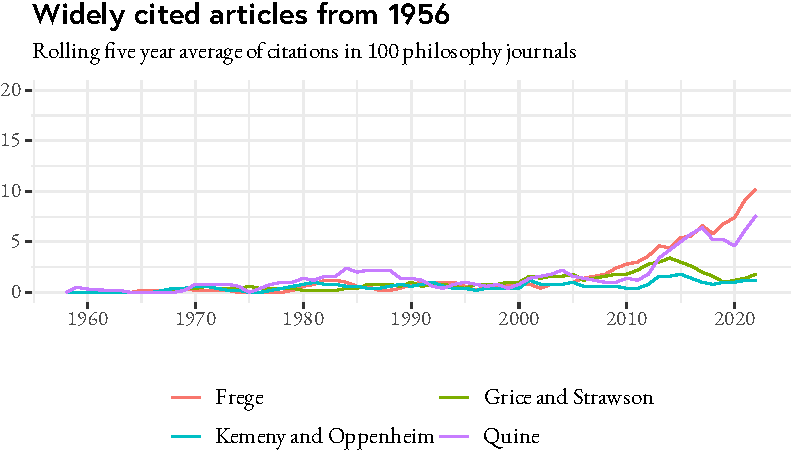
\includegraphics{citations_files/figure-pdf/fig-citation-spaghetti-1956-1.pdf}

}

\caption{\label{fig-citation-spaghetti-1956}Rolling five year average of
citation frequency for widely cited articles from 1956.}

\end{figure}%

\begin{figure}

\centering{

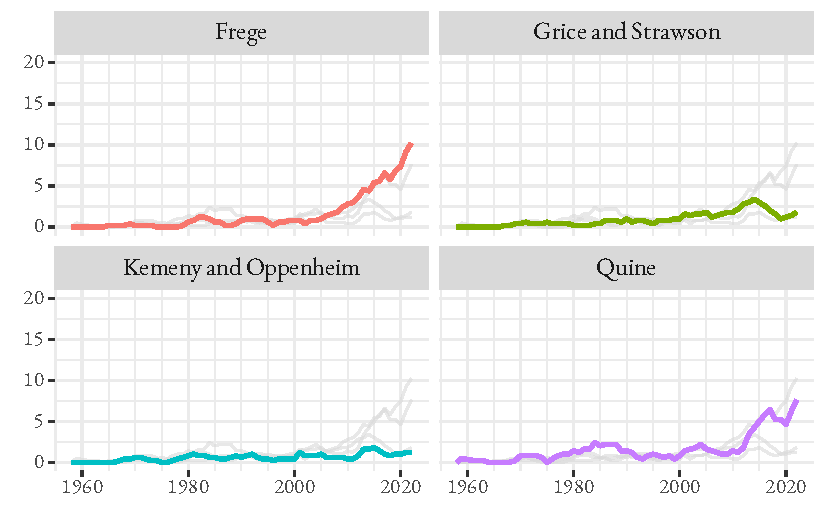
\includegraphics{citations_files/figure-pdf/fig-citation-facet-1956-1.pdf}

}

\caption{\label{fig-citation-facet-1956}Faceted version of
Figure~\ref{fig-citation-spaghetti-1956}.}

\end{figure}%

\newpage

\subsection{1957}\label{sec-s1957}

\subsubsection*{Widely Cited Articles}\label{widely-cited-articles-1}
\addcontentsline{toc}{subsubsection}{Widely Cited Articles}

\begin{enumerate}
\def\labelenumi{\arabic{enumi}.}
\tightlist
\item
  HP Grice (1957) ``Meaning,'' \emph{Philosophical Review}
  66~(3):~377-388.
\item
  Z Vendler (1957) ``Verbs and Times,'' \emph{Philosophical Review}
  66~(2):~143-160.
\end{enumerate}

\subsubsection*{Citation Count}\label{sec-count-1957}
\addcontentsline{toc}{subsubsection}{Citation Count}

\begin{longtable}[]{@{}lrrr@{}}

\caption{\label{tbl-citation-count-1957}Citation count for widely cited
articles from 1957.}

\tabularnewline

\toprule\noalign{}
Article & All & Early & Late \\
\midrule\noalign{}
\endhead
\bottomrule\noalign{}
\endlastfoot
Grice & 298 & 0 & 159 \\
Vendler & 58 & 0 & 46 \\

\end{longtable}

\subsubsection*{Citation Rank}\label{sec-rank-1957}
\addcontentsline{toc}{subsubsection}{Citation Rank}

\begin{longtable}[]{@{}lrrr@{}}

\caption{\label{tbl-citation-rank-1957}Citation rank for widely cited
articles from 1957.}

\tabularnewline

\toprule\noalign{}
Article & Overall & Early & Late \\
\midrule\noalign{}
\endhead
\bottomrule\noalign{}
\endlastfoot
Grice & 1 & 54 & 1 \\
Vendler & 2 & 54 & 2 \\

\end{longtable}

\subsubsection*{Citation Trends}\label{sec-trends-1957}
\addcontentsline{toc}{subsubsection}{Citation Trends}

\begin{figure}

\centering{

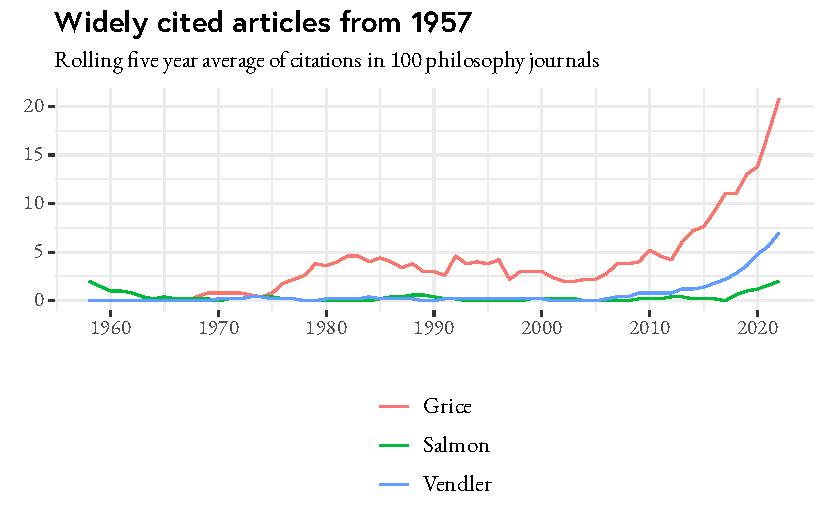
\includegraphics{citations_files/figure-pdf/fig-citation-spaghetti-1957-1.pdf}

}

\caption{\label{fig-citation-spaghetti-1957}Rolling five year average of
citation frequency for widely cited articles from 1957.}

\end{figure}%

\begin{figure}

\centering{

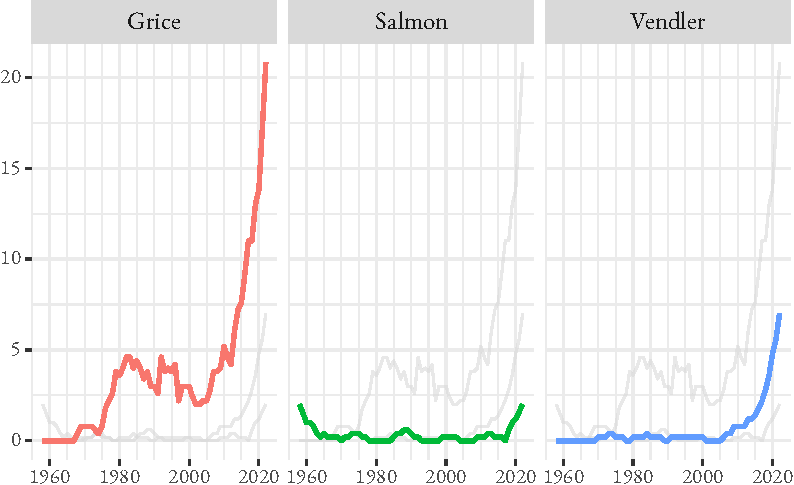
\includegraphics{citations_files/figure-pdf/fig-citation-facet-1957-1.pdf}

}

\caption{\label{fig-citation-facet-1957}Faceted version of
Figure~\ref{fig-citation-spaghetti-1957}.}

\end{figure}%

\newpage

\subsection{1958}\label{sec-s1958}

\subsubsection*{Widely Cited Articles}\label{widely-cited-articles-2}
\addcontentsline{toc}{subsubsection}{Widely Cited Articles}

\begin{enumerate}
\def\labelenumi{\arabic{enumi}.}
\tightlist
\item
  GEM Anscombe (1958) ``Modern Moral Philosophy,'' \emph{Philosophy}
  33~(124):~1-19.
\item
  JR Searle (1958) ``Proper Names,'' \emph{Mind} 67~(266):~166-173.
\item
  J Rawls (1958) ``Justice as Fairness,'' \emph{Philosophical Review}
  67~(2):~164-194.
\end{enumerate}

\subsubsection*{Citation Count}\label{sec-count-1958}
\addcontentsline{toc}{subsubsection}{Citation Count}

\begin{longtable}[]{@{}lrrr@{}}

\caption{\label{tbl-citation-count-1958}Citation count for widely cited
articles from 1958.}

\tabularnewline

\toprule\noalign{}
Article & All & Early & Late \\
\midrule\noalign{}
\endhead
\bottomrule\noalign{}
\endlastfoot
Anscombe & 194 & 3 & 107 \\
Searle & 83 & 2 & 24 \\
Rawls & 53 & 7 & 14 \\

\end{longtable}

\subsubsection*{Citation Rank}\label{sec-rank-1958}
\addcontentsline{toc}{subsubsection}{Citation Rank}

\begin{longtable}[]{@{}lrrr@{}}

\caption{\label{tbl-citation-rank-1958}Citation rank for widely cited
articles from 1958.}

\tabularnewline

\toprule\noalign{}
Article & Overall & Early & Late \\
\midrule\noalign{}
\endhead
\bottomrule\noalign{}
\endlastfoot
Anscombe & 1 & 4 & 1 \\
Searle & 2 & 11 & 2 \\
Rawls & 3 & 2 & 5 \\

\end{longtable}

\subsubsection*{Citation Trends}\label{sec-trends-1958}
\addcontentsline{toc}{subsubsection}{Citation Trends}

\begin{figure}

\centering{

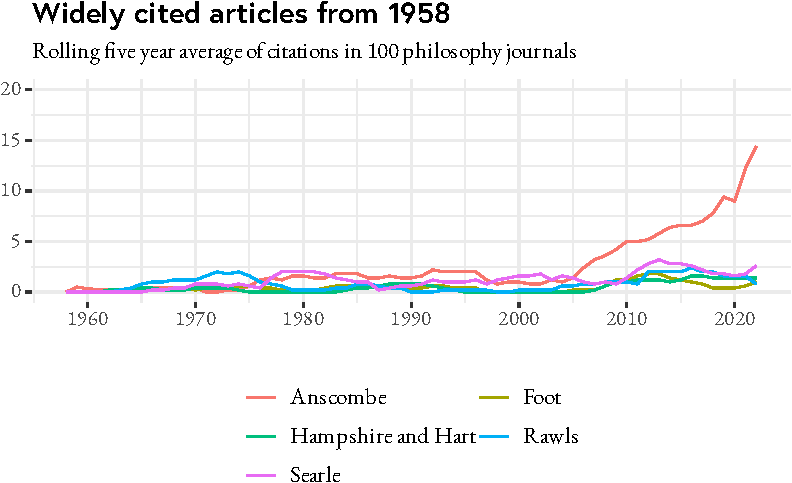
\includegraphics{citations_files/figure-pdf/fig-citation-spaghetti-1958-1.pdf}

}

\caption{\label{fig-citation-spaghetti-1958}Rolling five year average of
citation frequency for widely cited articles from 1958.}

\end{figure}%

\begin{figure}

\centering{

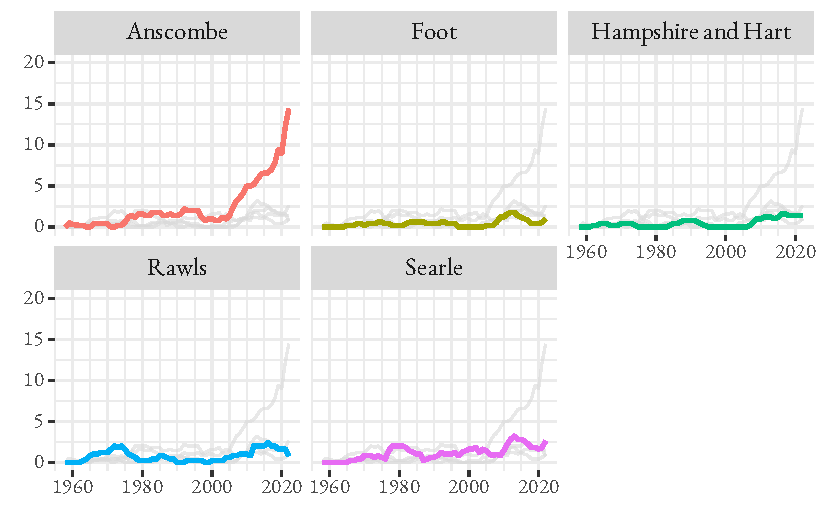
\includegraphics{citations_files/figure-pdf/fig-citation-facet-1958-1.pdf}

}

\caption{\label{fig-citation-facet-1958}Faceted version of
Figure~\ref{fig-citation-spaghetti-1958}.}

\end{figure}%

\newpage

\subsection{1959}\label{sec-s1959}

\subsubsection*{Widely Cited Articles}\label{widely-cited-articles-3}
\addcontentsline{toc}{subsubsection}{Widely Cited Articles}

\begin{enumerate}
\def\labelenumi{\arabic{enumi}.}
\tightlist
\item
  JJC Smart (1959) ``Sensations and Brain Processes,''
  \emph{Philosophical Review} 68~(2):~141-156.
\item
  F Sibley (1959) ``Aesthetic Concepts,'' \emph{Philosophical Review}
  68~(4):~421-450.
\item
  AN Prior (1959) ``Thank Goodness That's Over,'' \emph{Philosophy}
  34~(128):~12-17.
\item
  KR Popper (1959) ``The Propensity Interpretation of Probability,''
  \emph{British Journal For The Philosophy Of Science} 10~(37):~25-42.
\item
  M Dummett (1959) ``Wittgenstein's Philosophy of Mathematics,''
  \emph{Philosophical Review} 68~(3):~324-348.
\end{enumerate}

\subsubsection*{Citation Count}\label{sec-count-1959}
\addcontentsline{toc}{subsubsection}{Citation Count}

\begin{longtable}[]{@{}lrrr@{}}

\caption{\label{tbl-citation-count-1959}Citation count for widely cited
articles from 1959.}

\tabularnewline

\toprule\noalign{}
Article & All & Early & Late \\
\midrule\noalign{}
\endhead
\bottomrule\noalign{}
\endlastfoot
Smart & 180 & 9 & 85 \\
Sibley & 93 & 2 & 56 \\
Prior & 87 & 0 & 60 \\
Popper & 63 & 1 & 18 \\
Dummett & 39 & 4 & 20 \\

\end{longtable}

\subsubsection*{Citation Rank}\label{sec-rank-1959}
\addcontentsline{toc}{subsubsection}{Citation Rank}

\begin{longtable}[]{@{}lrrr@{}}

\caption{\label{tbl-citation-rank-1959}Citation rank for widely cited
articles from 1959.}

\tabularnewline

\toprule\noalign{}
Article & Overall & Early & Late \\
\midrule\noalign{}
\endhead
\bottomrule\noalign{}
\endlastfoot
Smart & 1 & 1 & 1 \\
Sibley & 2 & 11 & 3 \\
Prior & 3 & 61 & 2 \\
Popper & 4 & 22 & 5 \\
Dummett & 5 & 4 & 4 \\

\end{longtable}

\subsubsection*{Citation Trends}\label{sec-trends-1959}
\addcontentsline{toc}{subsubsection}{Citation Trends}

\begin{figure}

\centering{

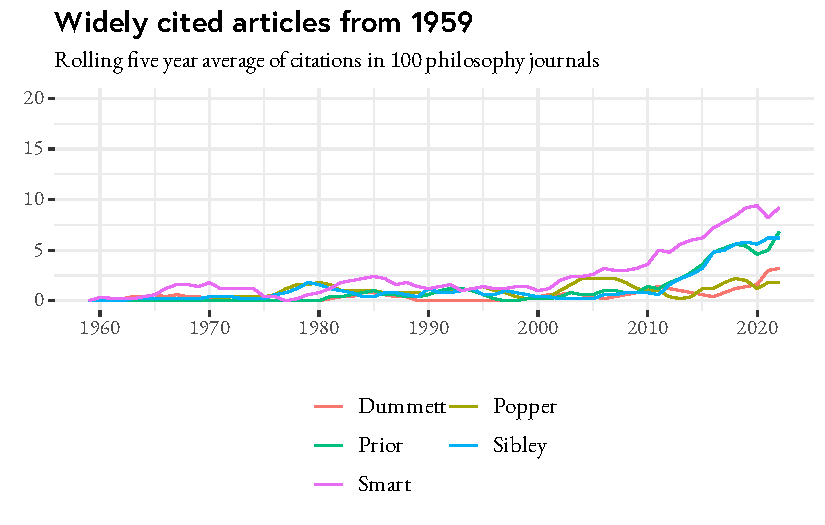
\includegraphics{citations_files/figure-pdf/fig-citation-spaghetti-1959-1.pdf}

}

\caption{\label{fig-citation-spaghetti-1959}Rolling five year average of
citation frequency for widely cited articles from 1959.}

\end{figure}%

\begin{figure}

\centering{

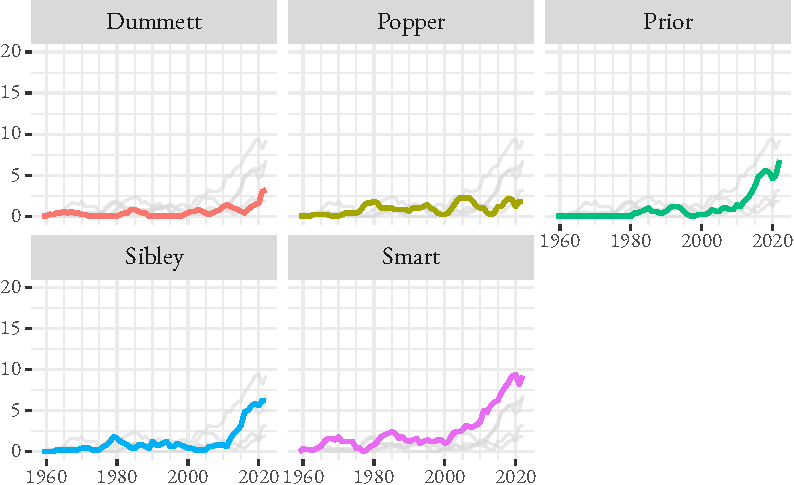
\includegraphics{citations_files/figure-pdf/fig-citation-facet-1959-1.pdf}

}

\caption{\label{fig-citation-facet-1959}Faceted version of
Figure~\ref{fig-citation-spaghetti-1959}.}

\end{figure}%

\newpage

\subsection{1960}\label{sec-s1960}

\subsubsection*{Widely Cited Articles}\label{widely-cited-articles-4}
\addcontentsline{toc}{subsubsection}{Widely Cited Articles}

\begin{enumerate}
\def\labelenumi{\arabic{enumi}.}
\tightlist
\item
  PT Geach (1960) ``Ascriptivism,'' \emph{Philosophical Review}
  69~(2):~221-225.
\item
  N Malcolm (1960) ``Anselm's Ontological Arguments,''
  \emph{Philosophical Review} 69~(1):~41-62.
\end{enumerate}

\subsubsection*{Citation Count}\label{sec-count-1960}
\addcontentsline{toc}{subsubsection}{Citation Count}

\begin{longtable}[]{@{}lrrr@{}}

\caption{\label{tbl-citation-count-1960}Citation count for widely cited
articles from 1960.}

\tabularnewline

\toprule\noalign{}
Article & All & Early & Late \\
\midrule\noalign{}
\endhead
\bottomrule\noalign{}
\endlastfoot
Geach & 68 & 2 & 29 \\
Malcolm & 67 & 14 & 18 \\

\end{longtable}

\subsubsection*{Citation Rank}\label{sec-rank-1960}
\addcontentsline{toc}{subsubsection}{Citation Rank}

\begin{longtable}[]{@{}lrrr@{}}

\caption{\label{tbl-citation-rank-1960}Citation rank for widely cited
articles from 1960.}

\tabularnewline

\toprule\noalign{}
Article & Overall & Early & Late \\
\midrule\noalign{}
\endhead
\bottomrule\noalign{}
\endlastfoot
Geach & 1 & 6 & 1 \\
Malcolm & 2 & 1 & 3 \\

\end{longtable}

\subsubsection*{Citation Trends}\label{sec-trends-1960}
\addcontentsline{toc}{subsubsection}{Citation Trends}

\begin{figure}

\centering{

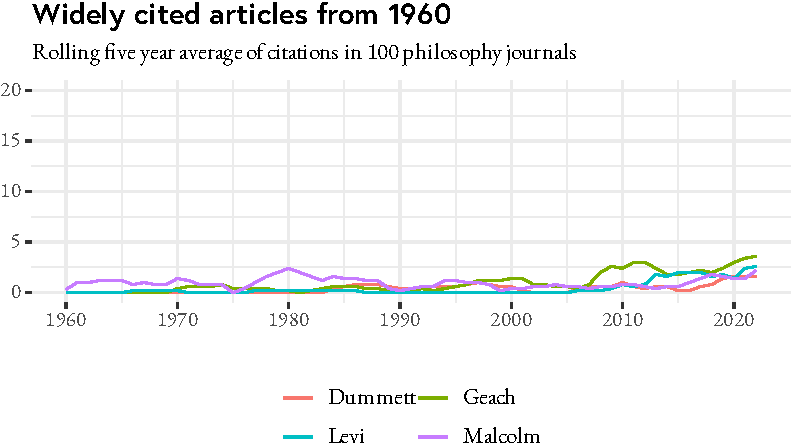
\includegraphics{citations_files/figure-pdf/fig-citation-spaghetti-1960-1.pdf}

}

\caption{\label{fig-citation-spaghetti-1960}Rolling five year average of
citation frequency for widely cited articles from 1960.}

\end{figure}%

\begin{figure}

\centering{

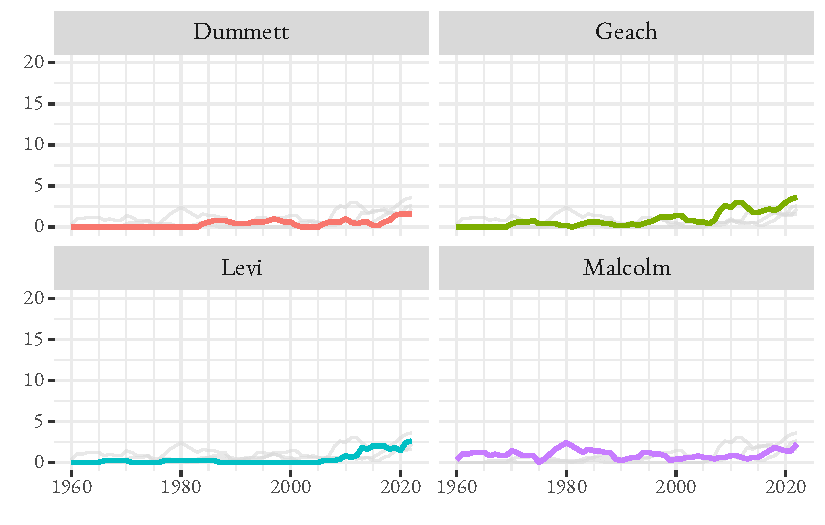
\includegraphics{citations_files/figure-pdf/fig-citation-facet-1960-1.pdf}

}

\caption{\label{fig-citation-facet-1960}Faceted version of
Figure~\ref{fig-citation-spaghetti-1960}.}

\end{figure}%

\newpage

\subsection{1961}\label{sec-s1961}

\subsubsection*{Widely Cited Articles}\label{widely-cited-articles-5}
\addcontentsline{toc}{subsubsection}{Widely Cited Articles}

\begin{enumerate}
\def\labelenumi{\arabic{enumi}.}
\tightlist
\item
  JJC Smart (1961) ``Free-Will, Praise and Blame,'' \emph{Mind}
  70~(279):~291-306.
\item
  JR Lucas (1961) ``Minds, Machines and Gödel,'' \emph{Philosophy}
  36~(137):~112-127.
\item
  IJ Good (1961) ``A Causal Calculus (I),'' \emph{British Journal For
  The Philosophy Of Science} 11~(44):~305-318.
\end{enumerate}

\subsubsection*{Citation Count}\label{sec-count-1961}
\addcontentsline{toc}{subsubsection}{Citation Count}

\begin{longtable}[]{@{}lrrr@{}}

\caption{\label{tbl-citation-count-1961}Citation count for widely cited
articles from 1961.}

\tabularnewline

\toprule\noalign{}
Article & All & Early & Late \\
\midrule\noalign{}
\endhead
\bottomrule\noalign{}
\endlastfoot
Smart & 68 & 2 & 39 \\
Lucas & 50 & 9 & 14 \\
Good & 46 & 0 & 16 \\

\end{longtable}

\subsubsection*{Citation Rank}\label{sec-rank-1961}
\addcontentsline{toc}{subsubsection}{Citation Rank}

\begin{longtable}[]{@{}lrrr@{}}

\caption{\label{tbl-citation-rank-1961}Citation rank for widely cited
articles from 1961.}

\tabularnewline

\toprule\noalign{}
Article & Overall & Early & Late \\
\midrule\noalign{}
\endhead
\bottomrule\noalign{}
\endlastfoot
Smart & 1 & 10 & 1 \\
Lucas & 2 & 1 & 4 \\
Good & 3 & 82 & 2 \\

\end{longtable}

\subsubsection*{Citation Trends}\label{sec-trends-1961}
\addcontentsline{toc}{subsubsection}{Citation Trends}

\begin{figure}

\centering{

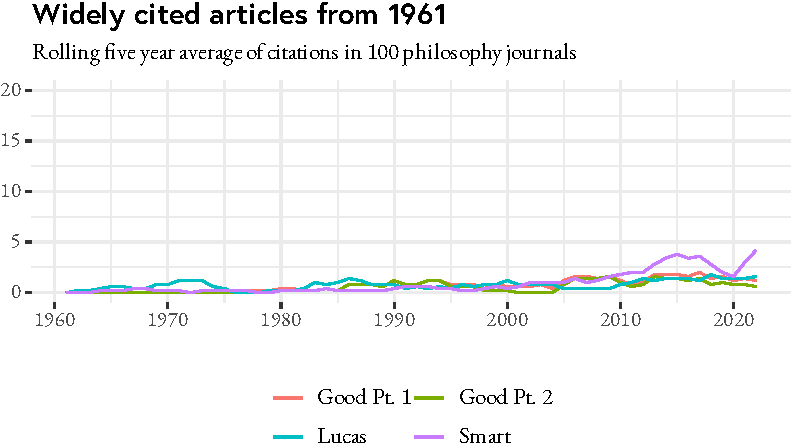
\includegraphics{citations_files/figure-pdf/fig-citation-spaghetti-1961-1.pdf}

}

\caption{\label{fig-citation-spaghetti-1961}Rolling five year average of
citation frequency for widely cited articles from 1961.}

\end{figure}%

\begin{figure}

\centering{

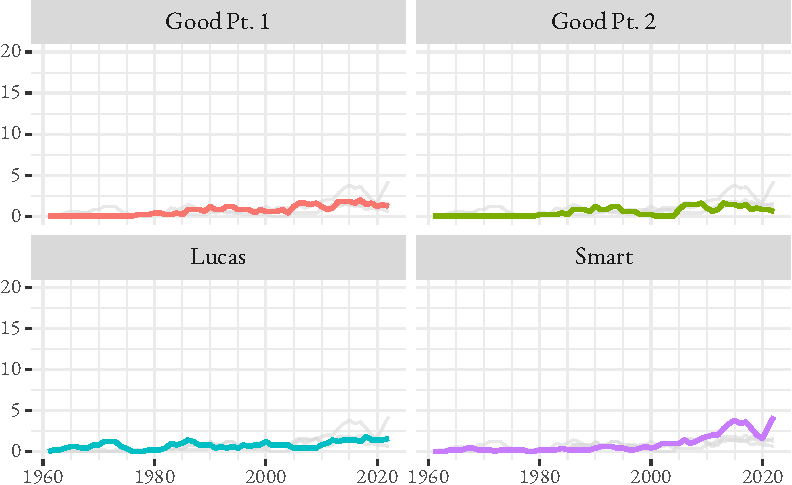
\includegraphics{citations_files/figure-pdf/fig-citation-facet-1961-1.pdf}

}

\caption{\label{fig-citation-facet-1961}Faceted version of
Figure~\ref{fig-citation-spaghetti-1961}.}

\end{figure}%

\newpage

\subsection{1962}\label{sec-s1962}

\subsubsection*{Widely Cited Articles}\label{widely-cited-articles-6}
\addcontentsline{toc}{subsubsection}{Widely Cited Articles}

\begin{enumerate}
\def\labelenumi{\arabic{enumi}.}
\tightlist
\item
  EJ Lemmon (1962) ``Moral Dilemmas,'' \emph{Philosophical Review}
  71~(2):~139-158.
\item
  H Putnam (1962) ``It Ain't Necessarily So,'' \emph{Journal Of
  Philosophy} 59~(22):~658-671.
\item
  JR Searle (1962) ``Meaning and Speech Acts,'' \emph{Philosophical
  Review} 71~(4):~423-432.
\item
  J Hintikka (1962) ``Cogito, Ergo Sum: Inference or Performance?,''
  \emph{Philosophical Review} 71~(1):~3-32.
\end{enumerate}

\subsubsection*{Citation Count}\label{sec-count-1962}
\addcontentsline{toc}{subsubsection}{Citation Count}

\begin{longtable}[]{@{}lrrr@{}}

\caption{\label{tbl-citation-count-1962}Citation count for widely cited
articles from 1962.}

\tabularnewline

\toprule\noalign{}
Article & All & Early & Late \\
\midrule\noalign{}
\endhead
\bottomrule\noalign{}
\endlastfoot
Lemmon & 40 & 1 & 13 \\
Putnam & 38 & 5 & 18 \\
Searle & 37 & 2 & 13 \\
Hintikka & 36 & 3 & 10 \\

\end{longtable}

\subsubsection*{Citation Rank}\label{sec-rank-1962}
\addcontentsline{toc}{subsubsection}{Citation Rank}

\begin{longtable}[]{@{}lrrr@{}}

\caption{\label{tbl-citation-rank-1962}Citation rank for widely cited
articles from 1962.}

\tabularnewline

\toprule\noalign{}
Article & Overall & Early & Late \\
\midrule\noalign{}
\endhead
\bottomrule\noalign{}
\endlastfoot
Lemmon & 1 & 25 & 2 \\
Putnam & 2 & 4 & 1 \\
Searle & 3 & 13 & 2 \\
Hintikka & 4 & 6 & 7 \\

\end{longtable}

\subsubsection*{Citation Trends}\label{sec-trends-1962}
\addcontentsline{toc}{subsubsection}{Citation Trends}

\begin{figure}

\centering{

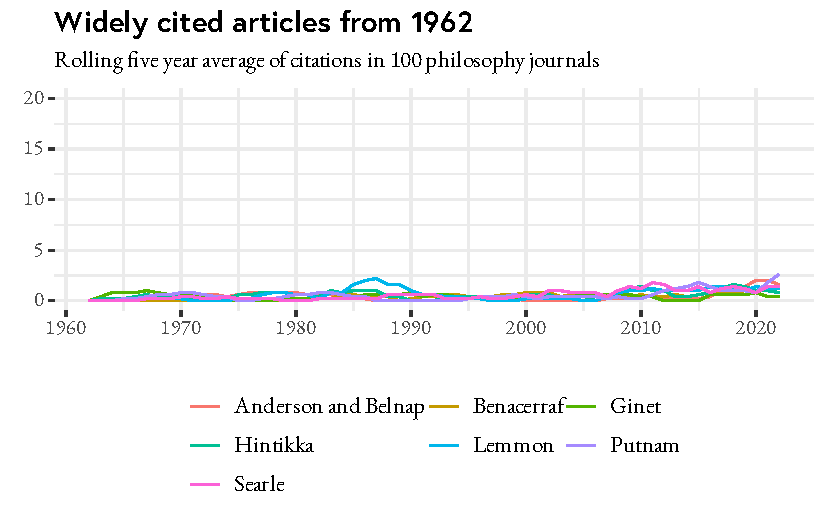
\includegraphics{citations_files/figure-pdf/fig-citation-spaghetti-1962-1.pdf}

}

\caption{\label{fig-citation-spaghetti-1962}Rolling five year average of
citation frequency for widely cited articles from 1962.}

\end{figure}%

\begin{figure}

\centering{

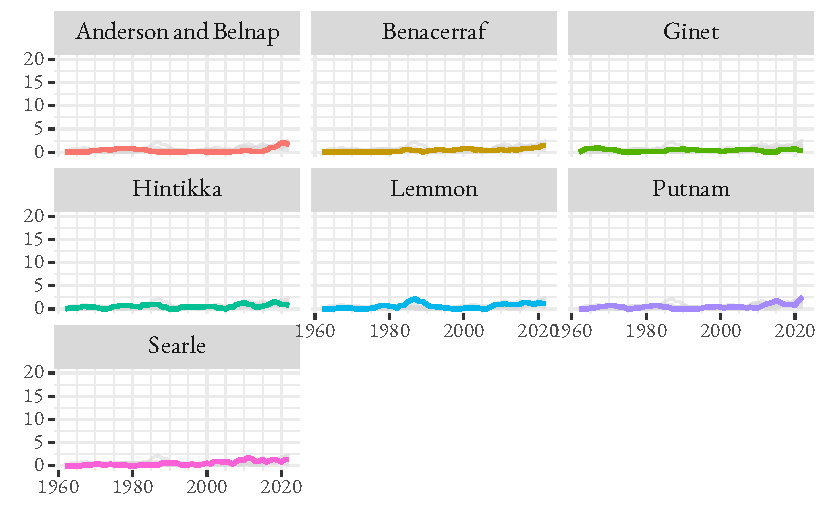
\includegraphics{citations_files/figure-pdf/fig-citation-facet-1962-1.pdf}

}

\caption{\label{fig-citation-facet-1962}Faceted version of
Figure~\ref{fig-citation-spaghetti-1962}.}

\end{figure}%

\newpage

\subsection{1963}\label{sec-s1963}

\subsubsection*{Widely Cited Articles}\label{widely-cited-articles-7}
\addcontentsline{toc}{subsubsection}{Widely Cited Articles}

\begin{enumerate}
\def\labelenumi{\arabic{enumi}.}
\tightlist
\item
  DM Armstrong (1963) ``Is Introspective Knowledge Incorrigible?,''
  \emph{Philosophical Review} 72~(4):~417-432.
\end{enumerate}

\subsubsection*{Citation Count}\label{sec-count-1963}
\addcontentsline{toc}{subsubsection}{Citation Count}

\begin{longtable}[]{@{}lrrr@{}}

\caption{\label{tbl-citation-count-1963}Citation count for widely cited
articles from 1963.}

\tabularnewline

\toprule\noalign{}
Article & All & Early & Late \\
\midrule\noalign{}
\endhead
\bottomrule\noalign{}
\endlastfoot
Armstrong & 32 & 2 & 15 \\

\end{longtable}

\subsubsection*{Citation Rank}\label{sec-rank-1963}
\addcontentsline{toc}{subsubsection}{Citation Rank}

\begin{longtable}[]{@{}lrrr@{}}

\caption{\label{tbl-citation-rank-1963}Citation rank for widely cited
articles from 1963.}

\tabularnewline

\toprule\noalign{}
Article & Overall & Early & Late \\
\midrule\noalign{}
\endhead
\bottomrule\noalign{}
\endlastfoot
Armstrong & 1 & 20 & 1 \\

\end{longtable}

\subsubsection*{Citation Trends}\label{sec-trends-1963}
\addcontentsline{toc}{subsubsection}{Citation Trends}

\begin{figure}

\centering{

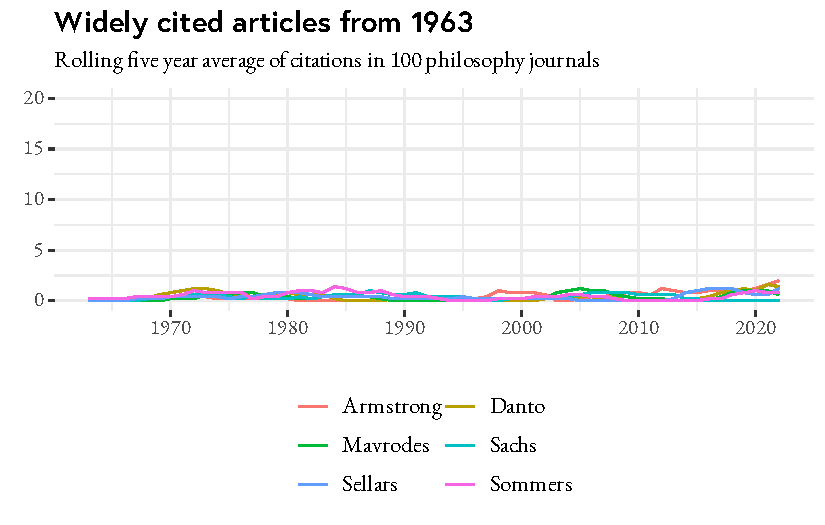
\includegraphics{citations_files/figure-pdf/fig-citation-spaghetti-1963-1.pdf}

}

\caption{\label{fig-citation-spaghetti-1963}Rolling five year average of
citation frequency for widely cited articles from 1963.}

\end{figure}%

\begin{figure}

\centering{

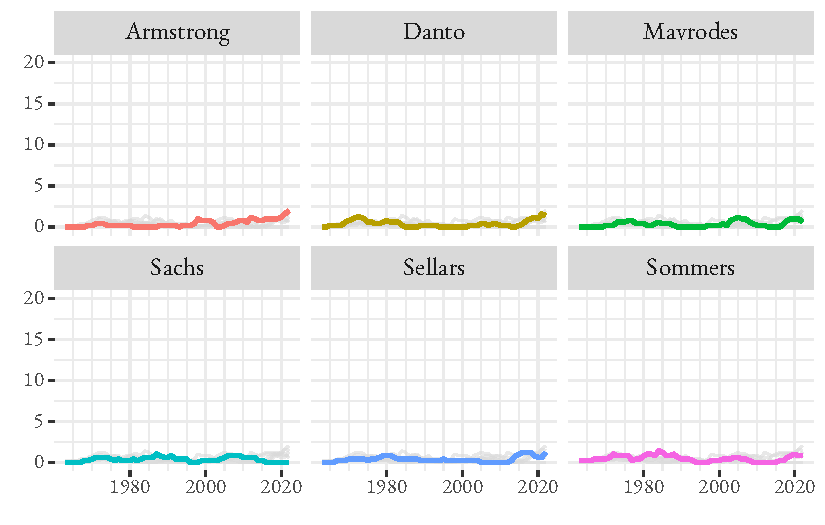
\includegraphics{citations_files/figure-pdf/fig-citation-facet-1963-1.pdf}

}

\caption{\label{fig-citation-facet-1963}Faceted version of
Figure~\ref{fig-citation-spaghetti-1963}.}

\end{figure}%

\newpage

\subsection{1964}\label{sec-s1964}

\subsubsection*{Widely Cited Articles}\label{widely-cited-articles-8}
\addcontentsline{toc}{subsubsection}{Widely Cited Articles}

\begin{enumerate}
\def\labelenumi{\arabic{enumi}.}
\tightlist
\item
  A Danto (1964) ``The Artworld,'' \emph{Journal Of Philosophy}
  61~(19):~571-584.
\item
  PF Strawson (1964) ``Intention and Convention in Speech Acts,''
  \emph{Philosophical Review} 73~(4):~439-460.
\item
  JR Searle (1964) ``How To Derive Ought From Is,'' \emph{Philosophical
  Review} 73~(1):~43-58.
\item
  M Dummett (1964) ``Bringing About the Past,'' \emph{Philosophical
  Review} 73~(3):~338-359.
\item
  G Dickie (1964) ``The Myth of the Aesthetic Attitude,'' \emph{American
  Philosophical Quarterly} 1~(1):~56-65.
\end{enumerate}

\subsubsection*{Citation Count}\label{sec-count-1964}
\addcontentsline{toc}{subsubsection}{Citation Count}

\begin{longtable}[]{@{}lrrr@{}}

\caption{\label{tbl-citation-count-1964}Citation count for widely cited
articles from 1964.}

\tabularnewline

\toprule\noalign{}
Article & All & Early & Late \\
\midrule\noalign{}
\endhead
\bottomrule\noalign{}
\endlastfoot
Danto & 89 & 2 & 34 \\
Strawson & 73 & 3 & 47 \\
Searle & 66 & 10 & 25 \\
Dummett & 47 & 1 & 20 \\
Dickie & 47 & 2 & 20 \\

\end{longtable}

\subsubsection*{Citation Rank}\label{sec-rank-1964}
\addcontentsline{toc}{subsubsection}{Citation Rank}

\begin{longtable}[]{@{}lrrr@{}}

\caption{\label{tbl-citation-rank-1964}Citation rank for widely cited
articles from 1964.}

\tabularnewline

\toprule\noalign{}
Article & Overall & Early & Late \\
\midrule\noalign{}
\endhead
\bottomrule\noalign{}
\endlastfoot
Danto & 1 & 22 & 2 \\
Strawson & 2 & 11 & 1 \\
Searle & 3 & 1 & 3 \\
Dummett & 4 & 42 & 4 \\
Dickie & 4 & 22 & 4 \\

\end{longtable}

\subsubsection*{Citation Trends}\label{sec-trends-1964}
\addcontentsline{toc}{subsubsection}{Citation Trends}

\begin{figure}

\centering{

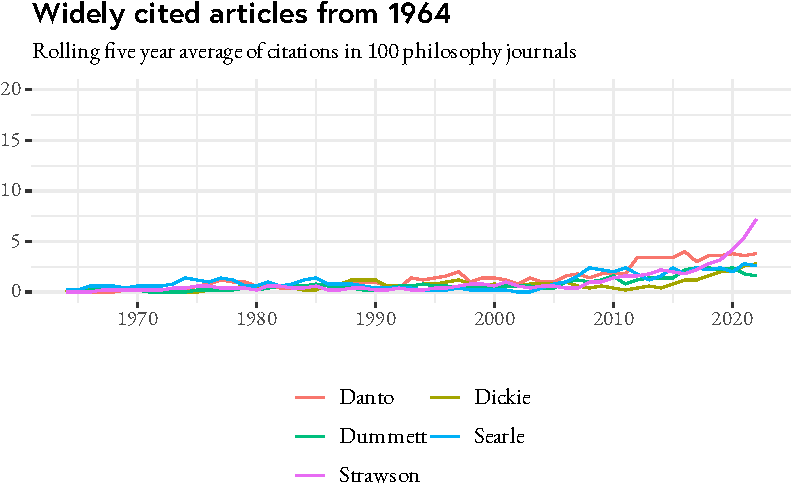
\includegraphics{citations_files/figure-pdf/fig-citation-spaghetti-1964-1.pdf}

}

\caption{\label{fig-citation-spaghetti-1964}Rolling five year average of
citation frequency for widely cited articles from 1964.}

\end{figure}%

\begin{figure}

\centering{

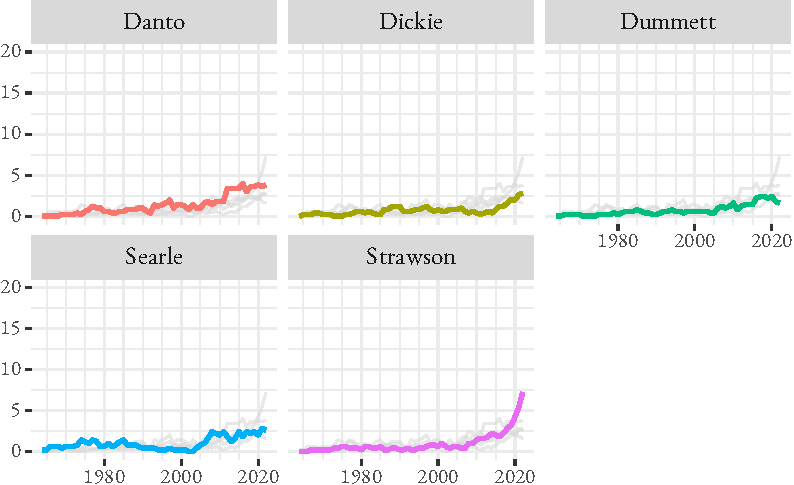
\includegraphics{citations_files/figure-pdf/fig-citation-facet-1964-1.pdf}

}

\caption{\label{fig-citation-facet-1964}Faceted version of
Figure~\ref{fig-citation-spaghetti-1964}.}

\end{figure}%

\newpage

\subsection{1965}\label{sec-s1965}

\subsubsection*{Widely Cited Articles}\label{widely-cited-articles-9}
\addcontentsline{toc}{subsubsection}{Widely Cited Articles}

\begin{enumerate}
\def\labelenumi{\arabic{enumi}.}
\tightlist
\item
  P Benacerraf (1965) ``What Numbers Could Not Be,'' \emph{Philosophical
  Review} 74~(1):~47-73.
\item
  GH Harman (1965) ``The Inference To the Best Explanation,''
  \emph{Philosophical Review} 74~(1):~88-95.
\item
  PT Geach (1965) ``Assertion,'' \emph{Philosophical Review}
  74~(4):~449-465.
\item
  JL Mackie (1965) ``Causes and Conditions,'' \emph{American
  Philosophical Quarterly} 2~(4):~245-264.
\item
  R Rorty (1965) ``Mind-Body Identity, Privacy, and Categories,''
  \emph{Review Of Metaphysics} 19~(1):~24-54.
\item
  DL Hull (1965) ``The Effect of Essentialism on Taxonomy---2000 Years
  of Stasis (1),'' \emph{British Journal For The Philosophy Of Science}
  15~(60):~314-326.
\item
  F Sibley (1965) ``Aesthetic and Non-Aesthetic,'' \emph{Philosophical
  Review} 74~(2):~135-159.
\item
  AC Danto (1965) ``Basic Actions,'' \emph{American Philosophical
  Quarterly} 2~(2):~141-148.
\item
  J Feinberg (1965) ``The Expressive Function of Punishment,''
  \emph{Monist} 49~(3):~397-423.
\end{enumerate}

\subsubsection*{Citation Count}\label{sec-count-1965}
\addcontentsline{toc}{subsubsection}{Citation Count}

\begin{longtable}[]{@{}lrrr@{}}

\caption{\label{tbl-citation-count-1965}Citation count for widely cited
articles from 1965.}

\tabularnewline

\toprule\noalign{}
Article & All & Early & Late \\
\midrule\noalign{}
\endhead
\bottomrule\noalign{}
\endlastfoot
Benacerraf & 228 & 5 & 113 \\
Harman & 190 & 10 & 84 \\
Geach & 159 & 2 & 72 \\
Mackie & 114 & 9 & 54 \\
Rorty & 61 & 21 & 11 \\
Hull & 52 & 0 & 18 \\
Sibley & 48 & 1 & 31 \\
Danto & 44 & 5 & 20 \\
Feinberg & 36 & 2 & 28 \\

\end{longtable}

\subsubsection*{Citation Rank}\label{sec-rank-1965}
\addcontentsline{toc}{subsubsection}{Citation Rank}

\begin{longtable}[]{@{}lrrr@{}}

\caption{\label{tbl-citation-rank-1965}Citation rank for widely cited
articles from 1965.}

\tabularnewline

\toprule\noalign{}
Article & Overall & Early & Late \\
\midrule\noalign{}
\endhead
\bottomrule\noalign{}
\endlastfoot
Benacerraf & 1 & 6 & 1 \\
Harman & 2 & 2 & 2 \\
Geach & 3 & 25 & 3 \\
Mackie & 4 & 3 & 4 \\
Rorty & 5 & 1 & 11 \\
Hull & 6 & 133 & 9 \\
Sibley & 7 & 52 & 5 \\
Danto & 9 & 6 & 8 \\
Feinberg & 11 & 25 & 6 \\

\end{longtable}

\subsubsection*{Citation Trends}\label{sec-trends-1965}
\addcontentsline{toc}{subsubsection}{Citation Trends}

\begin{figure}

\centering{

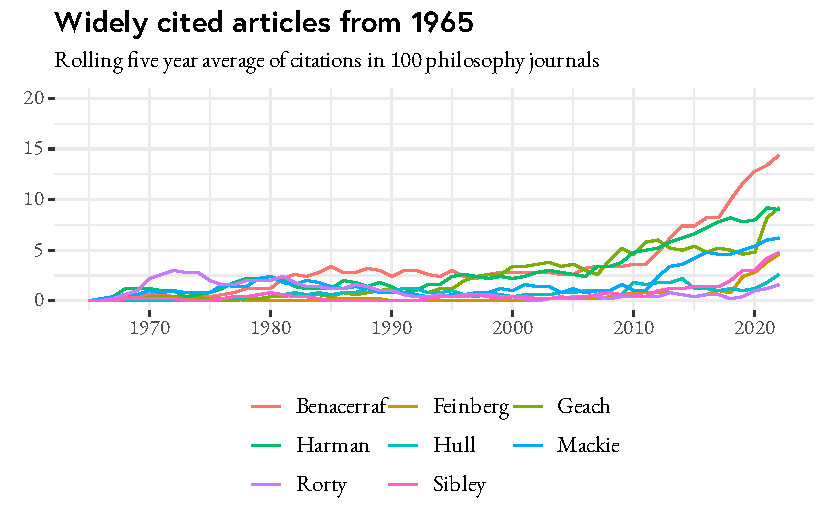
\includegraphics{citations_files/figure-pdf/fig-citation-spaghetti-1965-1.pdf}

}

\caption{\label{fig-citation-spaghetti-1965}Rolling five year average of
citation frequency for widely cited articles from 1965.}

\end{figure}%

\begin{figure}

\centering{

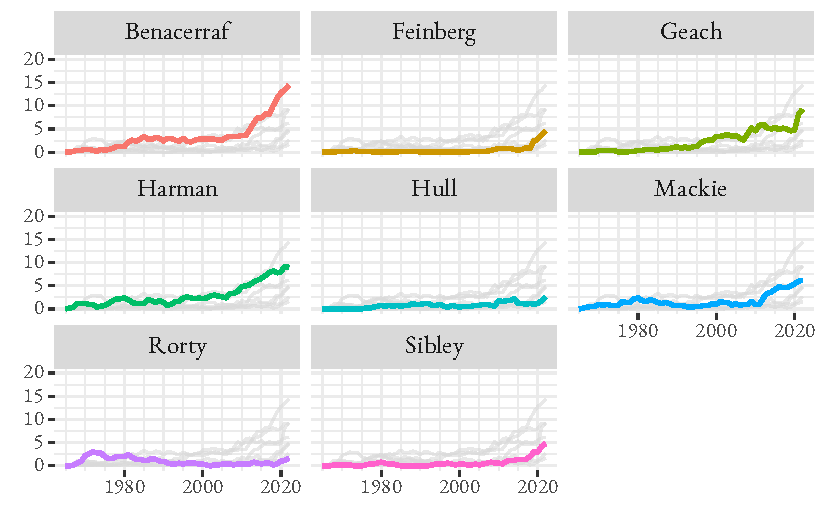
\includegraphics{citations_files/figure-pdf/fig-citation-facet-1965-1.pdf}

}

\caption{\label{fig-citation-facet-1965}Faceted version of
Figure~\ref{fig-citation-spaghetti-1965}.}

\end{figure}%

\newpage

\subsection{1966}\label{sec-s1966}

\subsubsection*{Widely Cited Articles}\label{widely-cited-articles-10}
\addcontentsline{toc}{subsubsection}{Widely Cited Articles}

\begin{enumerate}
\def\labelenumi{\arabic{enumi}.}
\tightlist
\item
  KS Donnellan (1966) ``Reference and Definite Descriptions,''
  \emph{Philosophical Review} 75~(3):~281-304.
\item
  DK Lewis (1966) ``An Argument for the Identity Theory,'' \emph{Journal
  Of Philosophy} 63~(1):~17-25.
\item
  CB Martin and M Deutscher (1966) ``Remembering,'' \emph{Philosophical
  Review} 75~(2):~161-196.
\item
  BC van Fraassen (1966) ``Singular Terms, Truth-Value Gaps, and Free
  Logic,'' \emph{Journal Of Philosophy} 63~(17):~481-495.
\item
  J Kim (1966) ``On the Psycho-Physical Identity Theory,''
  \emph{American Philosophical Quarterly} 3~(3):~227-235.
\end{enumerate}

\subsubsection*{Citation Count}\label{sec-count-1966}
\addcontentsline{toc}{subsubsection}{Citation Count}

\begin{longtable}[]{@{}lrrr@{}}

\caption{\label{tbl-citation-count-1966}Citation count for widely cited
articles from 1966.}

\tabularnewline

\toprule\noalign{}
Article & All & Early & Late \\
\midrule\noalign{}
\endhead
\bottomrule\noalign{}
\endlastfoot
Donnellan & 334 & 21 & 107 \\
Lewis & 141 & 3 & 61 \\
Martin and Deutscher & 81 & 3 & 50 \\
van Fraassen & 70 & 8 & 28 \\
Kim & 42 & 6 & 9 \\

\end{longtable}

\subsubsection*{Citation Rank}\label{sec-rank-1966}
\addcontentsline{toc}{subsubsection}{Citation Rank}

\begin{longtable}[]{@{}lrrr@{}}

\caption{\label{tbl-citation-rank-1966}Citation rank for widely cited
articles from 1966.}

\tabularnewline

\toprule\noalign{}
Article & Overall & Early & Late \\
\midrule\noalign{}
\endhead
\bottomrule\noalign{}
\endlastfoot
Donnellan & 1 & 1 & 1 \\
Lewis & 2 & 11 & 2 \\
Martin and Deutscher & 3 & 11 & 3 \\
van Fraassen & 4 & 2 & 4 \\
Kim & 5 & 4 & 8 \\

\end{longtable}

\subsubsection*{Citation Trends}\label{sec-trends-1966}
\addcontentsline{toc}{subsubsection}{Citation Trends}

\begin{figure}

\centering{

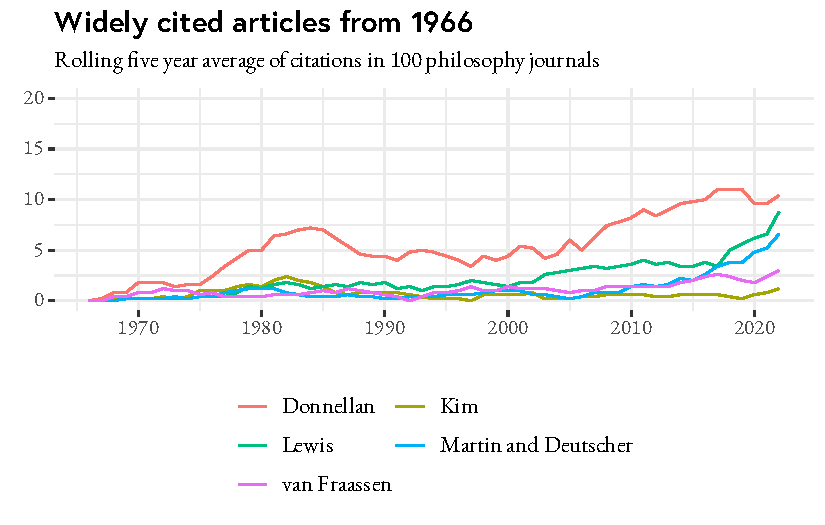
\includegraphics{citations_files/figure-pdf/fig-citation-spaghetti-1966-1.pdf}

}

\caption{\label{fig-citation-spaghetti-1966}Rolling five year average of
citation frequency for widely cited articles from 1966.}

\end{figure}%

\begin{figure}

\centering{

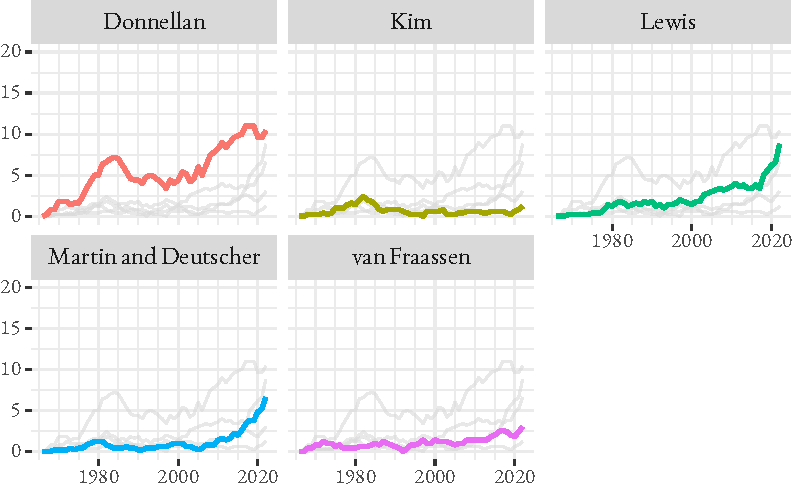
\includegraphics{citations_files/figure-pdf/fig-citation-facet-1966-1.pdf}

}

\caption{\label{fig-citation-facet-1966}Faceted version of
Figure~\ref{fig-citation-spaghetti-1966}.}

\end{figure}%

\newpage

\subsection{1967}\label{sec-s1967}

\subsubsection*{Widely Cited Articles}\label{widely-cited-articles-11}
\addcontentsline{toc}{subsubsection}{Widely Cited Articles}

\begin{enumerate}
\def\labelenumi{\arabic{enumi}.}
\tightlist
\item
  AI Goldman (1967) ``A Causal Theory of Knowing,'' \emph{Journal Of
  Philosophy} 64~(12):~357-372.
\item
  D Davidson (1967) ``Truth and Meaning,'' \emph{Synthese}
  17~(3):~304-323.
\item
  D Davidson (1967) ``Causal Relations,'' \emph{Journal Of Philosophy}
  64~(21):~691-703.
\item
  HN Castañeda (1967) ``Indicators and Quasi-Indicators,''
  \emph{American Philosophical Quarterly} 4~(2):~85-100.
\item
  KF Schaffner (1967) ``Approaches To Reduction,'' \emph{Philosophy Of
  Science} 34~(2):~137-147.
\item
  H Putnam (1967) ``Time and Physical Geometry,'' \emph{Journal Of
  Philosophy} 64~(8):~240-247.
\item
  I Hacking (1967) ``Slightly More Realistic Personal Probability,''
  \emph{Philosophy Of Science} 34~(4):~311-325.
\item
  I Hacking (1967) ``Possibility,'' \emph{Philosophical Review}
  76~(2):~143-168.
\end{enumerate}

\subsubsection*{Citation Count}\label{sec-count-1967}
\addcontentsline{toc}{subsubsection}{Citation Count}

\begin{longtable}[]{@{}lrrr@{}}

\caption{\label{tbl-citation-count-1967}Citation count for widely cited
articles from 1967.}

\tabularnewline

\toprule\noalign{}
Article & All & Early & Late \\
\midrule\noalign{}
\endhead
\bottomrule\noalign{}
\endlastfoot
Goldman & 161 & 16 & 77 \\
Davidson, Truth & 146 & 16 & 48 \\
Davidson, Causal & 133 & 17 & 44 \\
Castañeda & 99 & 12 & 19 \\
Schaffner & 98 & 6 & 22 \\
Putnam & 90 & 4 & 47 \\
Hacking, Probability & 62 & 4 & 28 \\
Hacking, Possibility & 59 & 3 & 33 \\

\end{longtable}

\subsubsection*{Citation Rank}\label{sec-rank-1967}
\addcontentsline{toc}{subsubsection}{Citation Rank}

\begin{longtable}[]{@{}lrrr@{}}

\caption{\label{tbl-citation-rank-1967}Citation rank for widely cited
articles from 1967.}

\tabularnewline

\toprule\noalign{}
Article & Overall & Early & Late \\
\midrule\noalign{}
\endhead
\bottomrule\noalign{}
\endlastfoot
Goldman & 1 & 2 & 1 \\
Davidson, Truth & 2 & 2 & 2 \\
Davidson, Causal & 3 & 1 & 4 \\
Castañeda & 4 & 4 & 12 \\
Schaffner & 5 & 9 & 10 \\
Putnam & 6 & 14 & 3 \\
Hacking, Probability & 8 & 14 & 6 \\
Hacking, Possibility & 9 & 26 & 5 \\

\end{longtable}

\subsubsection*{Citation Trends}\label{sec-trends-1967}
\addcontentsline{toc}{subsubsection}{Citation Trends}

\begin{figure}

\centering{

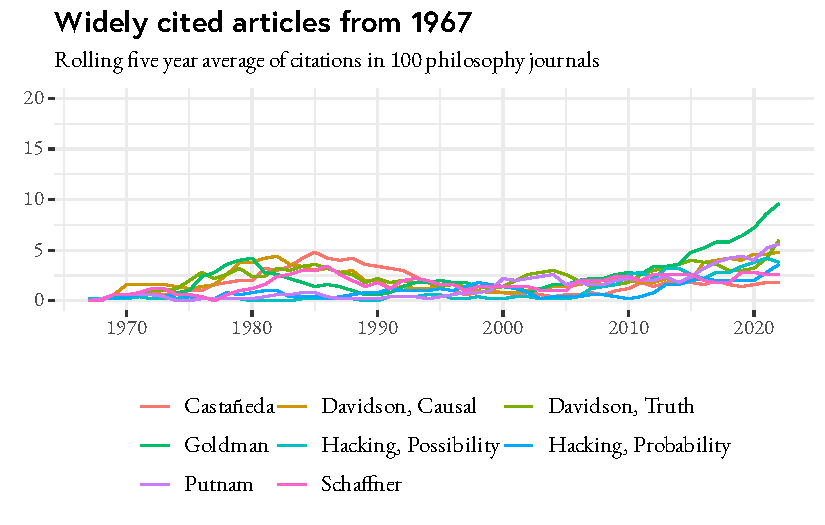
\includegraphics{citations_files/figure-pdf/fig-citation-spaghetti-1967-1.pdf}

}

\caption{\label{fig-citation-spaghetti-1967}Rolling five year average of
citation frequency for widely cited articles from 1967.}

\end{figure}%

\begin{figure}

\centering{

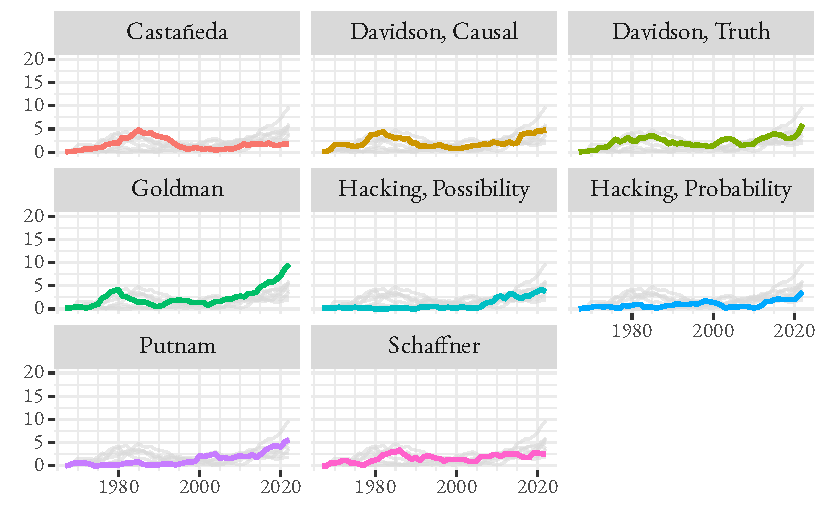
\includegraphics{citations_files/figure-pdf/fig-citation-facet-1967-1.pdf}

}

\caption{\label{fig-citation-facet-1967}Faceted version of
Figure~\ref{fig-citation-spaghetti-1967}.}

\end{figure}%

\newpage

\subsection{1968}\label{sec-s1968}

\subsubsection*{Widely Cited Articles}\label{widely-cited-articles-12}
\addcontentsline{toc}{subsubsection}{Widely Cited Articles}

\begin{enumerate}
\def\labelenumi{\arabic{enumi}.}
\tightlist
\item
  DK Lewis (1968) ``Counterpart Theory and Quantified Modal Logic,''
  \emph{Journal Of Philosophy} 65~(5):~113-126.
\item
  SS Shoemaker (1968) ``Self-Reference and Self-Awareness,''
  \emph{Journal Of Philosophy} 65~(19):~555-567.
\item
  B Stroud (1968) ``Transcendental Arguments,'' \emph{Journal Of
  Philosophy} 65~(9):~241-256.
\item
  P Unger (1968) ``An Analysis of Factual Knowledge,'' \emph{Journal Of
  Philosophy} 65~(6):~157-170.
\item
  H Morris (1968) ``Persons and Punishment,'' \emph{Monist}
  52~(4):~475-501.
\item
  BC van Fraassen (1968) ``Presupposition, Implication, and
  Self-Reference,'' \emph{Journal Of Philosophy} 65~(5):~136-151.
\item
  WV Quine (1968) ``Ontological Relativity,'' \emph{Journal Of
  Philosophy} 65~(7):~185-212.
\item
  G Harman (1968) ``Knowledge, Inference, and Explanation,''
  \emph{American Philosophical Quarterly} 5~(3):~164-173.
\end{enumerate}

\subsubsection*{Citation Count}\label{sec-count-1968}
\addcontentsline{toc}{subsubsection}{Citation Count}

\begin{longtable}[]{@{}lrrr@{}}

\caption{\label{tbl-citation-count-1968}Citation count for widely cited
articles from 1968.}

\tabularnewline

\toprule\noalign{}
Article & All & Early & Late \\
\midrule\noalign{}
\endhead
\bottomrule\noalign{}
\endlastfoot
Lewis & 216 & 8 & 94 \\
Shoemaker & 106 & 1 & 68 \\
Stroud & 103 & 10 & 40 \\
Unger & 90 & 10 & 49 \\
Morris & 65 & 3 & 20 \\
van Fraassen & 53 & 16 & 10 \\
Quine & 51 & 4 & 32 \\
Harman & 44 & 12 & 13 \\

\end{longtable}

\subsubsection*{Citation Rank}\label{sec-rank-1968}
\addcontentsline{toc}{subsubsection}{Citation Rank}

\begin{longtable}[]{@{}lrrr@{}}

\caption{\label{tbl-citation-rank-1968}Citation rank for widely cited
articles from 1968.}

\tabularnewline

\toprule\noalign{}
Article & Overall & Early & Late \\
\midrule\noalign{}
\endhead
\bottomrule\noalign{}
\endlastfoot
Lewis & 1 & 6 & 1 \\
Shoemaker & 2 & 56 & 2 \\
Stroud & 3 & 3 & 4 \\
Unger & 4 & 3 & 3 \\
Morris & 5 & 18 & 7 \\
van Fraassen & 7 & 1 & 15 \\
Quine & 8 & 13 & 5 \\
Harman & 9 & 2 & 12 \\

\end{longtable}

\subsubsection*{Citation Trends}\label{sec-trends-1968}
\addcontentsline{toc}{subsubsection}{Citation Trends}

\begin{figure}

\centering{

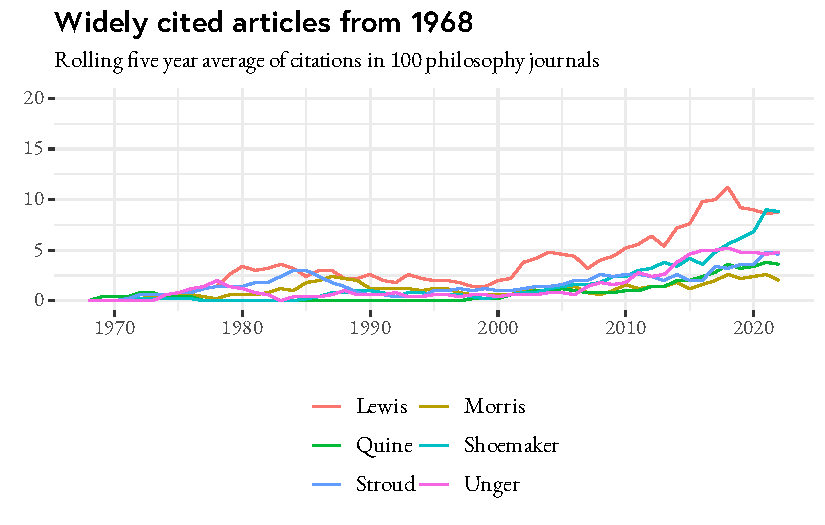
\includegraphics{citations_files/figure-pdf/fig-citation-spaghetti-1968-1.pdf}

}

\caption{\label{fig-citation-spaghetti-1968}Rolling five year average of
citation frequency for widely cited articles from 1968.}

\end{figure}%

\begin{figure}

\centering{

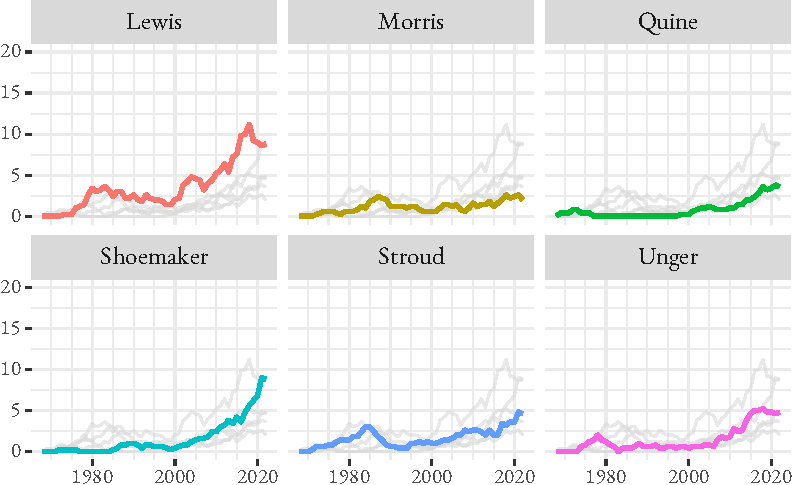
\includegraphics{citations_files/figure-pdf/fig-citation-facet-1968-1.pdf}

}

\caption{\label{fig-citation-facet-1968}Faceted version of
Figure~\ref{fig-citation-spaghetti-1968}.}

\end{figure}%

\newpage

\subsection{1969}\label{sec-s1969}

\subsubsection*{Widely Cited Articles}\label{widely-cited-articles-13}
\addcontentsline{toc}{subsubsection}{Widely Cited Articles}

\begin{enumerate}
\def\labelenumi{\arabic{enumi}.}
\tightlist
\item
  HG Frankfurt (1969) ``Alternate Possibilities and Moral
  Responsibility,'' \emph{Journal Of Philosophy} 66~(23):~829-839.
\item
  K Lehrer and T Paxson (1969) ``Knowledge: Undefeated Justified True
  Belief,'' \emph{Journal Of Philosophy} 66~(8):~225-237.
\item
  HP Grice (1969) ``Utterer's Meaning and Intentions,''
  \emph{Philosophical Review} 78~(2):~147-177.
\item
  BC van Fraassen (1969) ``Facts and Tautological Entailments,''
  \emph{Journal Of Philosophy} 66~(15):~477-487.
\item
  S Shoemaker (1969) ``Time Without Change,'' \emph{Journal Of
  Philosophy} 66~(12):~363-381.
\item
  JA Goguen (1969) ``The Logic of Inexact Concepts,'' \emph{Synthese}
  19~(3-4):~325-373.
\end{enumerate}

\subsubsection*{Citation Count}\label{sec-count-1969}
\addcontentsline{toc}{subsubsection}{Citation Count}

\begin{longtable}[]{@{}lrrr@{}}

\caption{\label{tbl-citation-count-1969}Citation count for widely cited
articles from 1969.}

\tabularnewline

\toprule\noalign{}
Article & All & Early & Late \\
\midrule\noalign{}
\endhead
\bottomrule\noalign{}
\endlastfoot
Frankfurt & 500 & 4 & 272 \\
Lehrer and Paxson & 100 & 12 & 44 \\
Grice & 91 & 9 & 35 \\
van Fraassen & 53 & 4 & 31 \\
Shoemaker & 45 & 3 & 17 \\
Goguen & 45 & 2 & 11 \\

\end{longtable}

\subsubsection*{Citation Rank}\label{sec-rank-1969}
\addcontentsline{toc}{subsubsection}{Citation Rank}

\begin{longtable}[]{@{}lrrr@{}}

\caption{\label{tbl-citation-rank-1969}Citation rank for widely cited
articles from 1969.}

\tabularnewline

\toprule\noalign{}
Article & Overall & Early & Late \\
\midrule\noalign{}
\endhead
\bottomrule\noalign{}
\endlastfoot
Frankfurt & 1 & 10 & 1 \\
Lehrer and Paxson & 2 & 1 & 2 \\
Grice & 3 & 2 & 3 \\
van Fraassen & 4 & 10 & 4 \\
Shoemaker & 5 & 22 & 8 \\
Goguen & 5 & 35 & 10 \\

\end{longtable}

\subsubsection*{Citation Trends}\label{sec-trends-1969}
\addcontentsline{toc}{subsubsection}{Citation Trends}

\begin{figure}

\centering{

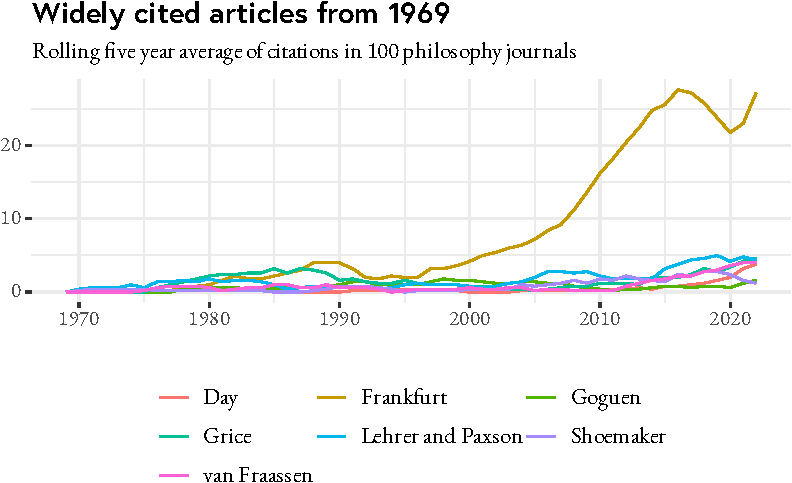
\includegraphics{citations_files/figure-pdf/fig-citation-spaghetti-1969-1.pdf}

}

\caption{\label{fig-citation-spaghetti-1969}Rolling five year average of
citation frequency for widely cited articles from 1969.}

\end{figure}%

\begin{figure}

\centering{

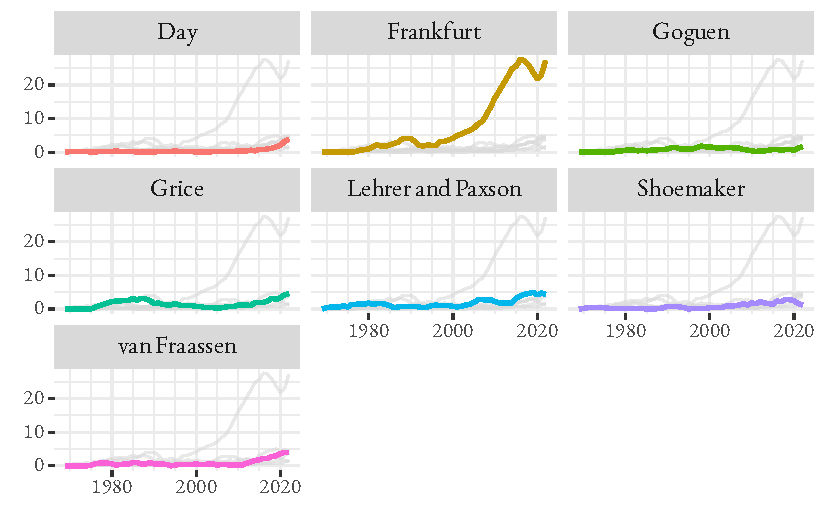
\includegraphics{citations_files/figure-pdf/fig-citation-facet-1969-1.pdf}

}

\caption{\label{fig-citation-facet-1969}Faceted version of
Figure~\ref{fig-citation-spaghetti-1969}.}

\end{figure}%

\newpage

\subsection{1970}\label{sec-s1970}

\subsubsection*{Widely Cited Articles}\label{widely-cited-articles-14}
\addcontentsline{toc}{subsubsection}{Widely Cited Articles}

\begin{enumerate}
\def\labelenumi{\arabic{enumi}.}
\tightlist
\item
  FI Dretske (1970) ``Epistemic Operators,'' \emph{Journal Of
  Philosophy} 67~(24):~1007-1023.
\item
  D Lewis (1970) ``How To Define Theoretical Terms,'' \emph{Journal Of
  Philosophy} 67~(13):~427-446.
\item
  KL Walton (1970) ``Categories of Art,'' \emph{Philosophical Review}
  79~(3):~334-367.
\item
  S Shoemaker (1970) ``Persons and Their Pasts,'' \emph{American
  Philosophical Quarterly} 7~(4):~269-285.
\item
  R Stalnaker (1970) ``Probability and Conditionals,'' \emph{Philosophy
  Of Science} 37~(1):~64-80.
\item
  WV Quine (1970) ``On the Reasons for Indeterminacy of Translation,''
  \emph{Journal Of Philosophy} 67~(6):~178-183.
\item
  VANFRAAS.BC NA (1970) ``On Extension of Beths Semantics of Physical
  Theories,'' \emph{Philosophy Of Science} 37~(3):~325-\&.
\item
  R Rorty (1970) ``Incorrigibility as Mark of Mental,'' \emph{Journal Of
  Philosophy} 67~(12):~399-424.
\end{enumerate}

\subsubsection*{Citation Count}\label{sec-count-1970}
\addcontentsline{toc}{subsubsection}{Citation Count}

\begin{longtable}[]{@{}lrrr@{}}

\caption{\label{tbl-citation-count-1970}Citation count for widely cited
articles from 1970.}

\tabularnewline

\toprule\noalign{}
Article & All & Early & Late \\
\midrule\noalign{}
\endhead
\bottomrule\noalign{}
\endlastfoot
Dretske & 331 & 3 & 159 \\
Lewis & 233 & 5 & 113 \\
Walton & 174 & 4 & 96 \\
Shoemaker & 92 & 3 & 43 \\
Stalnaker & 87 & 5 & 45 \\
Quine & 68 & 17 & 12 \\
NA & 50 & 8 & 17 \\
Rorty & 35 & 12 & 5 \\

\end{longtable}

\subsubsection*{Citation Rank}\label{sec-rank-1970}
\addcontentsline{toc}{subsubsection}{Citation Rank}

\begin{longtable}[]{@{}lrrr@{}}

\caption{\label{tbl-citation-rank-1970}Citation rank for widely cited
articles from 1970.}

\tabularnewline

\toprule\noalign{}
Article & Overall & Early & Late \\
\midrule\noalign{}
\endhead
\bottomrule\noalign{}
\endlastfoot
Dretske & 1 & 33 & 1 \\
Lewis & 2 & 16 & 2 \\
Walton & 3 & 24 & 3 \\
Shoemaker & 4 & 33 & 5 \\
Stalnaker & 5 & 16 & 4 \\
Quine & 6 & 1 & 15 \\
NA & 9 & 4 & 9 \\
Rorty & 12 & 2 & 23 \\

\end{longtable}

\subsubsection*{Citation Trends}\label{sec-trends-1970}
\addcontentsline{toc}{subsubsection}{Citation Trends}

\begin{figure}

\centering{

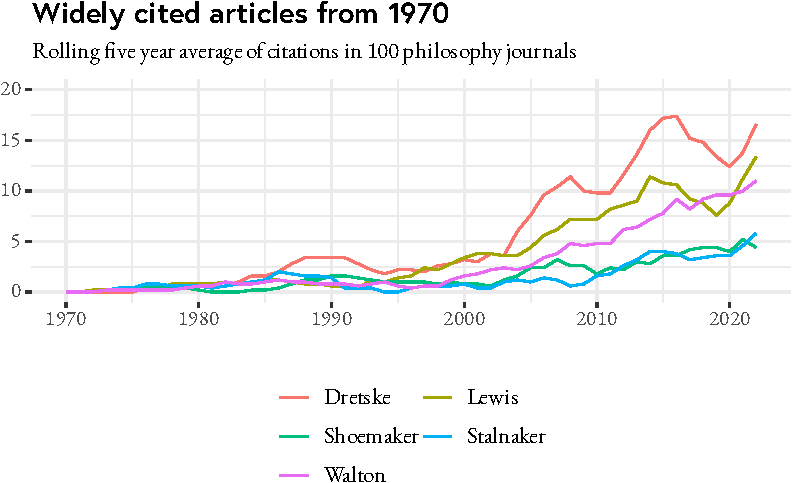
\includegraphics{citations_files/figure-pdf/fig-citation-spaghetti-1970-1.pdf}

}

\caption{\label{fig-citation-spaghetti-1970}Rolling five year average of
citation frequency for widely cited articles from 1970.}

\end{figure}%

\begin{figure}

\centering{

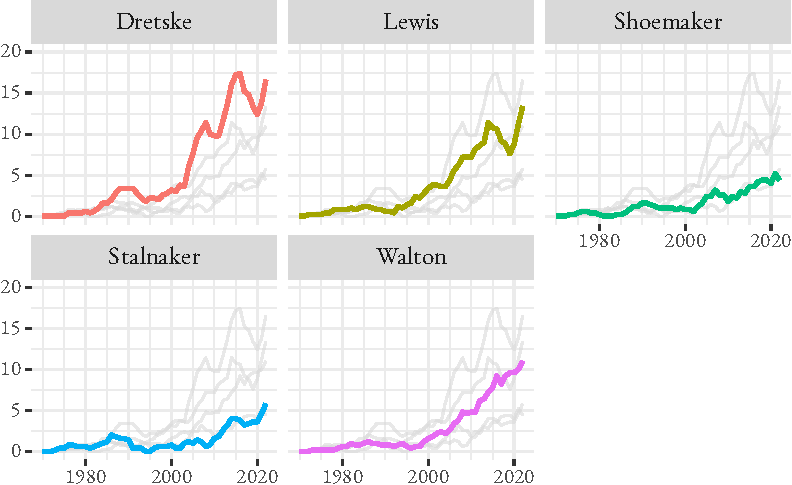
\includegraphics{citations_files/figure-pdf/fig-citation-facet-1970-1.pdf}

}

\caption{\label{fig-citation-facet-1970}Faceted version of
Figure~\ref{fig-citation-spaghetti-1970}.}

\end{figure}%

\newpage

\subsection{1971}\label{sec-s1971}

\subsubsection*{Widely Cited Articles}\label{widely-cited-articles-15}
\addcontentsline{toc}{subsubsection}{Widely Cited Articles}

\begin{enumerate}
\def\labelenumi{\arabic{enumi}.}
\tightlist
\item
  H Frankfurt (1971) ``Freedom of the Will and the Concept of a
  Person,'' \emph{Journal Of Philosophy} 68 (1): 5-20.
\item
  JJ Thomson (1971) ``A Defense of Abortion,'' \emph{Philosophy \&
  Public Affairs} 1~(1):~47-66.
\item
  D Parfit (1971) ``Personal Identity,'' \emph{Philosophical Review}
  80~(1):~3-27.
\item
  D Lewis (1971) ``Counterparts of Persons and Their Bodies,''
  \emph{Journal Of Philosophy} 68 (7): 203-211.
\item
  D Dennett (1971) ``Intentional Systems,'' \emph{Journal Of Philosophy}
  68 (4): 87-106.
\item
  G Boolos (1971) ``The Iterative Conception of Set,'' \emph{Journal Of
  Philosophy} 68 (8): 215-231.
\item
  P Klein (1971) ``A Proposed Definition of Propositional Knowledge,''
  \emph{Journal Of Philosophy} 68 (16): 471-482.
\item
  D Lewis (1971) ``Immodest Inductive Methods,'' \emph{Philosophy Of
  Science} 38~(1):~54-63.
\item
  A Goldman (1971) ``The Individuation of Action,'' \emph{Journal Of
  Philosophy} 68 (21): 761-774.
\end{enumerate}

\subsubsection*{Citation Count}\label{sec-count-1971}
\addcontentsline{toc}{subsubsection}{Citation Count}

\begin{longtable}[]{@{}lrrr@{}}

\caption{\label{tbl-citation-count-1971}Citation count for widely cited
articles from 1971.}

\tabularnewline

\toprule\noalign{}
Article & All & Early & Late \\
\midrule\noalign{}
\endhead
\bottomrule\noalign{}
\endlastfoot
Frankfurt & 508 & 34 & 224 \\
Thomson & 231 & 20 & 117 \\
Parfit & 141 & 16 & 58 \\
Lewis & 109 & 9 & 47 \\
Dennett & 103 & 17 & 30 \\
Boolos & 85 & 4 & 46 \\
Klein & 47 & 13 & 16 \\
Lewis, Inductive & 41 & 2 & 35 \\
Goldman & 40 & 17 & 8 \\

\end{longtable}

\subsubsection*{Citation Rank}\label{sec-rank-1971}
\addcontentsline{toc}{subsubsection}{Citation Rank}

\begin{longtable}[]{@{}lrrr@{}}

\caption{\label{tbl-citation-rank-1971}Citation rank for widely cited
articles from 1971.}

\tabularnewline

\toprule\noalign{}
Article & Overall & Early & Late \\
\midrule\noalign{}
\endhead
\bottomrule\noalign{}
\endlastfoot
Frankfurt & 1 & 1 & 1 \\
Thomson & 2 & 2 & 2 \\
Parfit & 3 & 5 & 3 \\
Lewis & 4 & 8 & 4 \\
Dennett & 5 & 3 & 7 \\
Boolos & 6 & 27 & 5 \\
Klein & 9 & 6 & 12 \\
Lewis, Inductive & 10 & 53 & 6 \\
Goldman & 12 & 3 & 18 \\

\end{longtable}

\subsubsection*{Citation Trends}\label{sec-trends-1971}
\addcontentsline{toc}{subsubsection}{Citation Trends}

\begin{figure}

\centering{

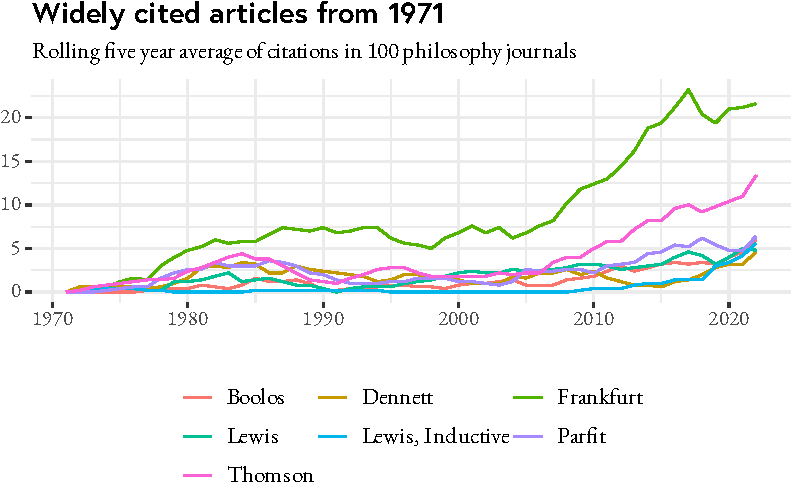
\includegraphics{citations_files/figure-pdf/fig-citation-spaghetti-1971-1.pdf}

}

\caption{\label{fig-citation-spaghetti-1971}Rolling five year average of
citation frequency for widely cited articles from 1971.}

\end{figure}%

\begin{figure}

\centering{

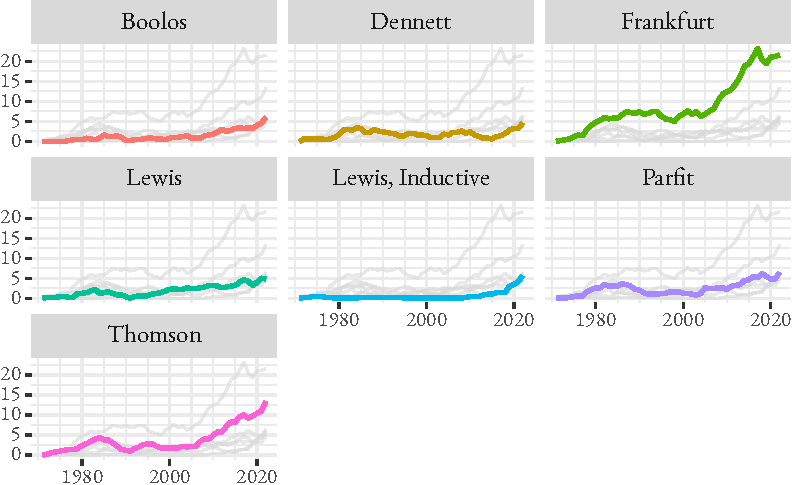
\includegraphics{citations_files/figure-pdf/fig-citation-facet-1971-1.pdf}

}

\caption{\label{fig-citation-facet-1971}Faceted version of
Figure~\ref{fig-citation-spaghetti-1971}.}

\end{figure}%

\newpage

\subsection{1972}\label{sec-s1972}

\subsubsection*{Widely Cited Articles}\label{widely-cited-articles-16}
\addcontentsline{toc}{subsubsection}{Widely Cited Articles}

\begin{enumerate}
\def\labelenumi{\arabic{enumi}.}
\tightlist
\item
  P Singer (1972) ``Famine, Affluence, and Morality,'' \emph{Philosophy
  \& Public Affairs} 1~(3):~229-243.
\item
  H Field (1972) ``Tarski's Theory of Truth,'' \emph{Journal Of
  Philosophy} 69 (13): 347-375.
\item
  P Foot (1972) ``Morality as a System of Hypothetical Imperatives,''
  \emph{Philosophical Review} 81~(3):~305-316.
\item
  NJ Block and JA Fodor (1972) ``What Psychological States Are Not,''
  \emph{Philosophical Review} 81~(2):~159-181.
\item
  J Perry (1972) ``Can the Self Divide?,'' \emph{Journal Of Philosophy}
  69 (16): 463-488.
\item
  R Rorty (1972) ``The World Well Lost,'' \emph{Journal Of Philosophy}
  69 (19): 649-665.
\item
  R Routley and RK Meyer (1972) ``The Semantics of Entailment --- II,''
  \emph{Journal Of Philosophical Logic} 1~(1):~53-73.
\item
  G Dworkin (1972) ``Paternalism,'' \emph{Monist} 56~(1):~64-84.
\end{enumerate}

\subsubsection*{Citation Count}\label{sec-count-1972}
\addcontentsline{toc}{subsubsection}{Citation Count}

\begin{longtable}[]{@{}lrrr@{}}

\caption{\label{tbl-citation-count-1972}Citation count for widely cited
articles from 1972.}

\tabularnewline

\toprule\noalign{}
Article & All & Early & Late \\
\midrule\noalign{}
\endhead
\bottomrule\noalign{}
\endlastfoot
Singer & 362 & 5 & 259 \\
Field & 134 & 29 & 21 \\
Foot & 132 & 17 & 76 \\
Block and Fodor & 84 & 13 & 23 \\
Perry & 63 & 12 & 12 \\
Rorty & 50 & 22 & 2 \\
Routley and Meyer & 39 & 3 & 24 \\
Dworkin & 36 & 3 & 28 \\

\end{longtable}

\subsubsection*{Citation Rank}\label{sec-rank-1972}
\addcontentsline{toc}{subsubsection}{Citation Rank}

\begin{longtable}[]{@{}lrrr@{}}

\caption{\label{tbl-citation-rank-1972}Citation rank for widely cited
articles from 1972.}

\tabularnewline

\toprule\noalign{}
Article & Overall & Early & Late \\
\midrule\noalign{}
\endhead
\bottomrule\noalign{}
\endlastfoot
Singer & 1 & 26 & 1 \\
Field & 2 & 1 & 6 \\
Foot & 3 & 4 & 2 \\
Block and Fodor & 4 & 5 & 5 \\
Perry & 5 & 7 & 13 \\
Rorty & 7 & 2 & 50 \\
Routley and Meyer & 11 & 42 & 4 \\
Dworkin & 13 & 42 & 3 \\

\end{longtable}

\subsubsection*{Citation Trends}\label{sec-trends-1972}
\addcontentsline{toc}{subsubsection}{Citation Trends}

\begin{figure}

\centering{

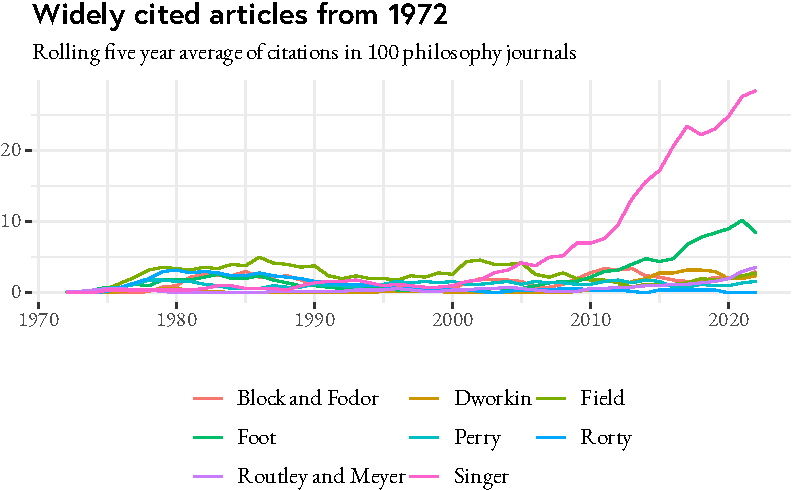
\includegraphics{citations_files/figure-pdf/fig-citation-spaghetti-1972-1.pdf}

}

\caption{\label{fig-citation-spaghetti-1972}Rolling five year average of
citation frequency for widely cited articles from 1972.}

\end{figure}%

\begin{figure}

\centering{

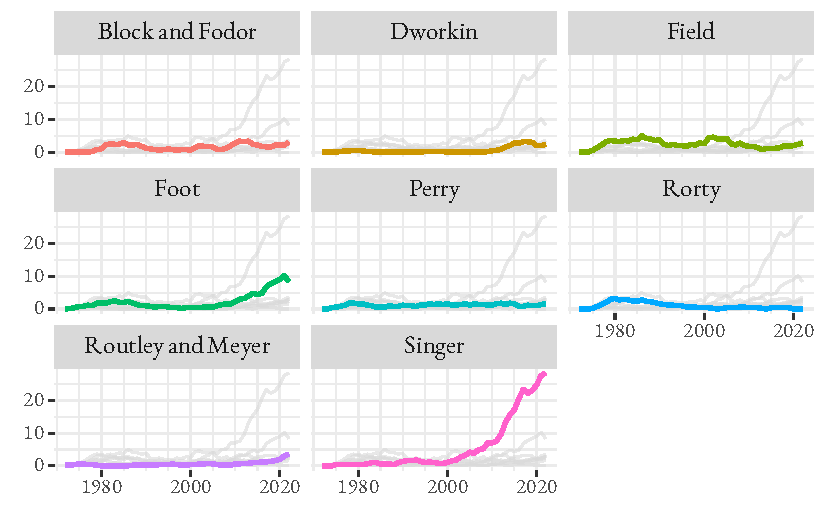
\includegraphics{citations_files/figure-pdf/fig-citation-facet-1972-1.pdf}

}

\caption{\label{fig-citation-facet-1972}Faceted version of
Figure~\ref{fig-citation-spaghetti-1972}.}

\end{figure}%

\newpage

\subsection{1973}\label{sec-s1973}

\subsubsection*{Widely Cited Articles}\label{widely-cited-articles-17}
\addcontentsline{toc}{subsubsection}{Widely Cited Articles}

\begin{enumerate}
\def\labelenumi{\arabic{enumi}.}
\tightlist
\item
  D Lewis (1973) ``Causation,'' \emph{Journal Of Philosophy} 70 (17):
  556-567.
\item
  P Benacerraf (1973) ``Mathematical Truth,'' \emph{Journal Of
  Philosophy} 70 (19): 661-679.
\item
  L Wright (1973) ``Functions,'' \emph{Philosophical Review}
  82~(2):~139-168.
\item
  H Putnam (1973) ``Meaning and Reference,'' \emph{Journal Of
  Philosophy} 70 (19): 699-711.
\item
  H Field (1973) ``Theory Change and the Indeterminacy of Reference,''
  \emph{Journal Of Philosophy} 70 (14): 462-481.
\item
  J Kim (1973) ``Causation, Nomic Subsumption, and the Concept of
  Event,'' \emph{Journal Of Philosophy} 70 (8): 217-236.
\item
  T Burge (1973) ``Reference and Proper Names,'' \emph{Journal Of
  Philosophy} 70 (14): 425-439.
\item
  M Walzer (1973) ``Political Action: The Problem of Dirty Hands,''
  \emph{Philosophy \& Public Affairs} 2~(2):~160-180.
\item
  E Zahar (1973) ``Why Did Einsteins Programme Supersede Lorentz's
  (1),'' \emph{British Journal For The Philosophy Of Science}
  24~(2):~95-123.
\end{enumerate}

\subsubsection*{Citation Count}\label{sec-count-1973}
\addcontentsline{toc}{subsubsection}{Citation Count}

\begin{longtable}[]{@{}lrrr@{}}

\caption{\label{tbl-citation-count-1973}Citation count for widely cited
articles from 1973.}

\tabularnewline

\toprule\noalign{}
Article & All & Early & Late \\
\midrule\noalign{}
\endhead
\bottomrule\noalign{}
\endlastfoot
Lewis & 447 & 43 & 226 \\
Benacerraf & 284 & 28 & 143 \\
Wright & 190 & 12 & 81 \\
Putnam & 165 & 39 & 79 \\
Field & 135 & 21 & 36 \\
Kim & 102 & 30 & 21 \\
Burge & 87 & 16 & 47 \\
Walzer & 61 & 5 & 37 \\
Zahar & 51 & 18 & 11 \\

\end{longtable}

\subsubsection*{Citation Rank}\label{sec-rank-1973}
\addcontentsline{toc}{subsubsection}{Citation Rank}

\begin{longtable}[]{@{}lrrr@{}}

\caption{\label{tbl-citation-rank-1973}Citation rank for widely cited
articles from 1973.}

\tabularnewline

\toprule\noalign{}
Article & Overall & Early & Late \\
\midrule\noalign{}
\endhead
\bottomrule\noalign{}
\endlastfoot
Lewis & 1 & 1 & 1 \\
Benacerraf & 2 & 4 & 2 \\
Wright & 3 & 10 & 3 \\
Putnam & 4 & 2 & 4 \\
Field & 5 & 5 & 7 \\
Kim & 6 & 3 & 12 \\
Burge & 7 & 8 & 5 \\
Walzer & 9 & 31 & 6 \\
Zahar & 13 & 6 & 19 \\

\end{longtable}

\subsubsection*{Citation Trends}\label{sec-trends-1973}
\addcontentsline{toc}{subsubsection}{Citation Trends}

\begin{figure}

\centering{

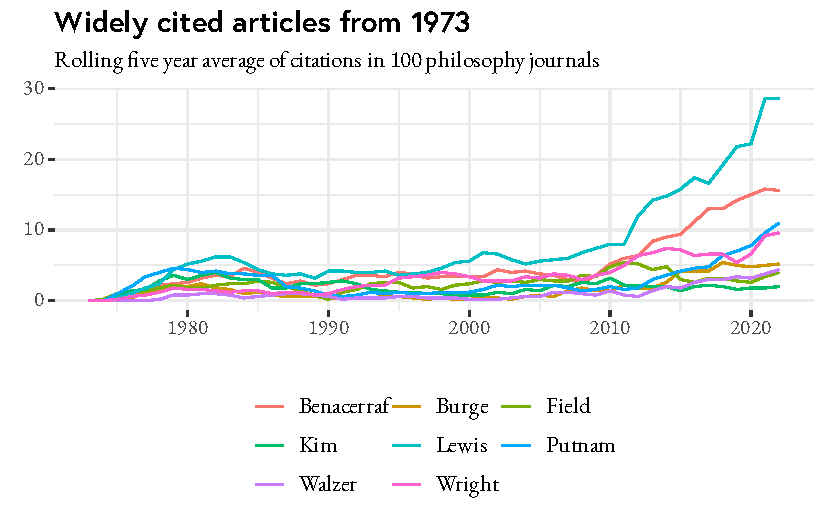
\includegraphics{citations_files/figure-pdf/fig-citation-spaghetti-1973-1.pdf}

}

\caption{\label{fig-citation-spaghetti-1973}Rolling five year average of
citation frequency for widely cited articles from 1973.}

\end{figure}%

\begin{figure}

\centering{

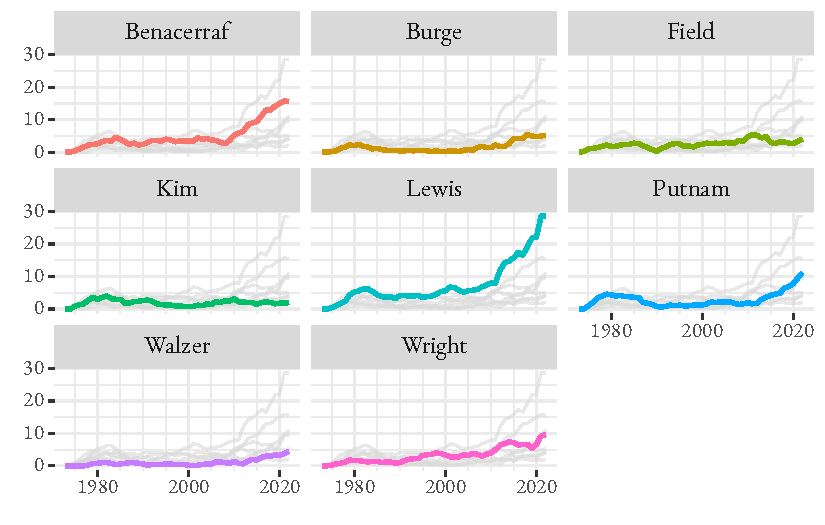
\includegraphics{citations_files/figure-pdf/fig-citation-facet-1973-1.pdf}

}

\caption{\label{fig-citation-facet-1973}Faceted version of
Figure~\ref{fig-citation-spaghetti-1973}.}

\end{figure}%

\newpage

\subsection{1974}\label{sec-s1974}

\subsubsection*{Widely Cited Articles}\label{widely-cited-articles-18}
\addcontentsline{toc}{subsubsection}{Widely Cited Articles}

\begin{enumerate}
\def\labelenumi{\arabic{enumi}.}
\tightlist
\item
  T Nagel (1974) ``What is It Like To Be a Bat,'' \emph{Philosophical
  Review} 83~(4):~435-450.
\item
  M Friedman (1974) ``Explanation and Scientific Understanding,''
  \emph{Journal Of Philosophy} 71 (1): 5-19.
\item
  I Levi (1974) ``On Indeterminate Probabilities,'' \emph{Journal Of
  Philosophy} 71 (13): 391-418.
\item
  KS Donnellan (1974) ``Speaking of Nothing,'' \emph{Philosophical
  Review} 83~(1):~3-31.
\item
  C Parsons (1974) ``The Liar Paradox,'' \emph{Journal Of Philosophical
  Logic} 3~(4):~381-412.
\item
  P Singer (1974) ``Sidgwick and Reflective Equilibrium,'' \emph{Monist}
  58~(3):~490-517.
\item
  M Devitt (1974) ``Singular Terms,'' \emph{Journal Of Philosophy} 71
  (7): 183-205.
\end{enumerate}

\subsubsection*{Citation Count}\label{sec-count-1974}
\addcontentsline{toc}{subsubsection}{Citation Count}

\begin{longtable}[]{@{}lrrr@{}}

\caption{\label{tbl-citation-count-1974}Citation count for widely cited
articles from 1974.}

\tabularnewline

\toprule\noalign{}
Article & All & Early & Late \\
\midrule\noalign{}
\endhead
\bottomrule\noalign{}
\endlastfoot
Nagel & 587 & 16 & 289 \\
Friedman & 232 & 12 & 115 \\
Levi & 122 & 12 & 67 \\
Donnellan & 77 & 19 & 26 \\
Parsons & 71 & 8 & 33 \\
Singer & 64 & 9 & 29 \\
Devitt & 49 & 26 & 11 \\

\end{longtable}

\subsubsection*{Citation Rank}\label{sec-rank-1974}
\addcontentsline{toc}{subsubsection}{Citation Rank}

\begin{longtable}[]{@{}lrrr@{}}

\caption{\label{tbl-citation-rank-1974}Citation rank for widely cited
articles from 1974.}

\tabularnewline

\toprule\noalign{}
Article & Overall & Early & Late \\
\midrule\noalign{}
\endhead
\bottomrule\noalign{}
\endlastfoot
Nagel & 1 & 3 & 1 \\
Friedman & 2 & 9 & 2 \\
Levi & 3 & 9 & 3 \\
Donnellan & 4 & 2 & 6 \\
Parsons & 5 & 20 & 4 \\
Singer & 6 & 16 & 5 \\
Devitt & 8 & 1 & 13 \\

\end{longtable}

\subsubsection*{Citation Trends}\label{sec-trends-1974}
\addcontentsline{toc}{subsubsection}{Citation Trends}

\begin{figure}

\centering{

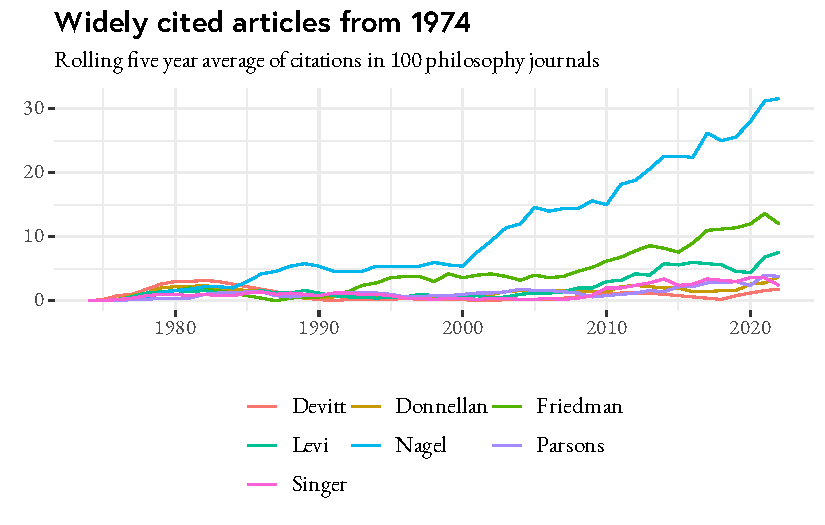
\includegraphics{citations_files/figure-pdf/fig-citation-spaghetti-1974-1.pdf}

}

\caption{\label{fig-citation-spaghetti-1974}Rolling five year average of
citation frequency for widely cited articles from 1974.}

\end{figure}%

\begin{figure}

\centering{

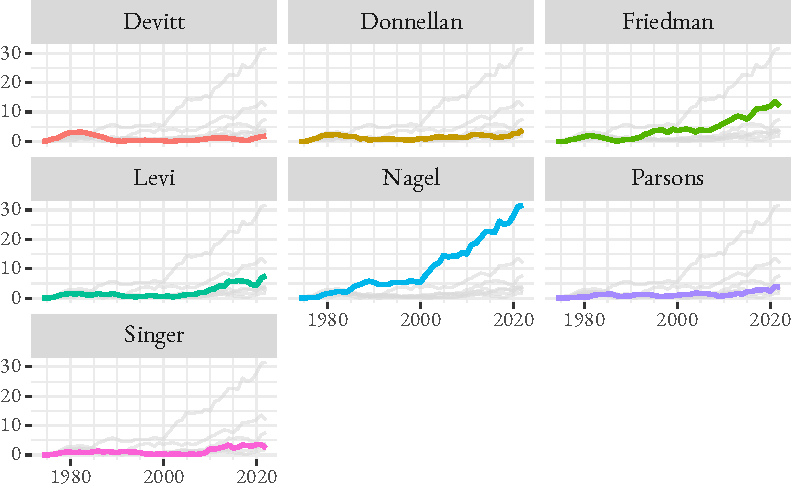
\includegraphics{citations_files/figure-pdf/fig-citation-facet-1974-1.pdf}

}

\caption{\label{fig-citation-facet-1974}Faceted version of
Figure~\ref{fig-citation-spaghetti-1974}.}

\end{figure}%

\newpage

\subsection{1975}\label{sec-s1975}

\subsubsection*{Widely Cited Articles}\label{widely-cited-articles-19}
\addcontentsline{toc}{subsubsection}{Widely Cited Articles}

\begin{enumerate}
\def\labelenumi{\arabic{enumi}.}
\tightlist
\item
  S Kripke (1975) ``Outline of a Theory of Truth,'' \emph{Journal Of
  Philosophy} 72~(19):~690-716.
\item
  R Cummins (1975) ``Functional Analysis,'' \emph{Journal Of Philosophy}
  72~(20):~741-765.
\item
  G Watson (1975) ``Free Agency,'' \emph{Journal Of Philosophy}
  72~(8):~205-220.
\item
  A Gibbard (1975) ``Contingent Identity,'' \emph{Journal Of
  Philosophical Logic} 4~(2):~187-221.
\item
  R Stalnaker (1975) ``Indicative Conditionals,'' \emph{Philosophia}
  5~(3):~269-286.
\item
  G Harman (1975) ``Moral Relativism Defended,'' \emph{Philosophical
  Review} 84~(1):~3-22.
\item
  DL Grover, JL Camp, and ND Belnap (1975) ``A Pro-Sentential Theory of
  Truth,'' \emph{Philosophical Studies} 27~(2):~73-125.
\item
  GP Hellman and FW Thompson (1975) ``Physicalism: Ontology,
  Determination, and Reduction,'' \emph{Journal Of Philosophy}
  72~(17):~551-564.
\item
  D Kaplan (1975) ``Sets, Concepts and Extensions: How To Russell a
  Frege-Church,'' \emph{Journal Of Philosophy} 72~(19):~716-729.
\end{enumerate}

\subsubsection*{Citation Count}\label{sec-count-1975}
\addcontentsline{toc}{subsubsection}{Citation Count}

\begin{longtable}[]{@{}lrrr@{}}

\caption{\label{tbl-citation-count-1975}Citation count for widely cited
articles from 1975.}

\tabularnewline

\toprule\noalign{}
Article & All & Early & Late \\
\midrule\noalign{}
\endhead
\bottomrule\noalign{}
\endlastfoot
Kripke & 430 & 43 & 218 \\
Cummins & 327 & 17 & 144 \\
Watson & 217 & 20 & 103 \\
Gibbard & 142 & 5 & 60 \\
Stalnaker & 114 & 3 & 86 \\
Harman & 106 & 14 & 45 \\
Grover et al & 86 & 14 & 22 \\
Hellman and Thompson & 67 & 19 & 6 \\
Kaplan & 66 & 14 & 18 \\

\end{longtable}

\subsubsection*{Citation Rank}\label{sec-rank-1975}
\addcontentsline{toc}{subsubsection}{Citation Rank}

\begin{longtable}[]{@{}lrrr@{}}

\caption{\label{tbl-citation-rank-1975}Citation rank for widely cited
articles from 1975.}

\tabularnewline

\toprule\noalign{}
Article & Overall & Early & Late \\
\midrule\noalign{}
\endhead
\bottomrule\noalign{}
\endlastfoot
Kripke & 1 & 1 & 1 \\
Cummins & 2 & 4 & 2 \\
Watson & 3 & 2 & 3 \\
Gibbard & 4 & 37 & 5 \\
Stalnaker & 5 & 67 & 4 \\
Harman & 6 & 5 & 6 \\
Grover et al & 7 & 5 & 10 \\
Hellman and Thompson & 8 & 3 & 34 \\
Kaplan & 9 & 5 & 16 \\

\end{longtable}

\subsubsection*{Citation Trends}\label{sec-trends-1975}
\addcontentsline{toc}{subsubsection}{Citation Trends}

\begin{figure}

\centering{

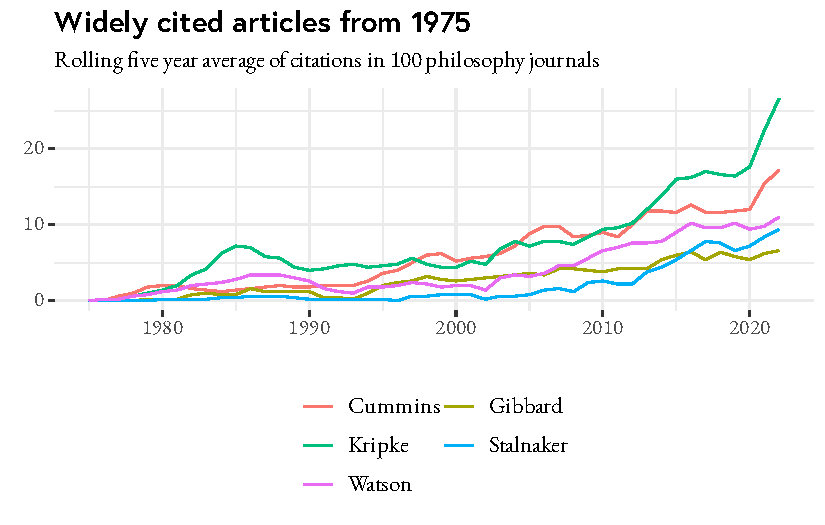
\includegraphics{citations_files/figure-pdf/fig-citation-spaghetti-1975-1.pdf}

}

\caption{\label{fig-citation-spaghetti-1975}Rolling five year average of
citation frequency for widely cited articles from 1975.}

\end{figure}%

\begin{figure}

\centering{

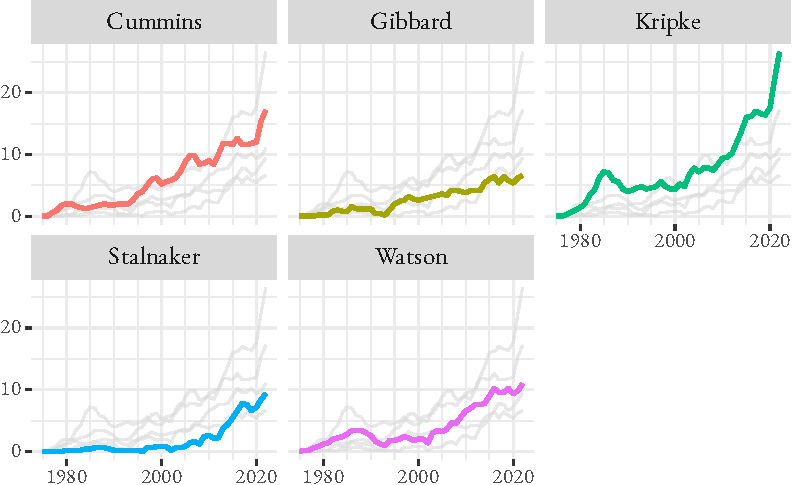
\includegraphics{citations_files/figure-pdf/fig-citation-facet-1975-1.pdf}

}

\caption{\label{fig-citation-facet-1975}Faceted version of
Figure~\ref{fig-citation-spaghetti-1975}.}

\end{figure}%

\newpage

\subsection{1976}\label{sec-s1976}

\subsubsection*{Widely Cited Articles}\label{widely-cited-articles-20}
\addcontentsline{toc}{subsubsection}{Widely Cited Articles}

\begin{enumerate}
\def\labelenumi{\arabic{enumi}.}
\tightlist
\item
  AI Goldman (1976) ``Discrimination and Perceptual Knowledge,''
  \emph{Journal Of Philosophy} 73~(20):~771-791.
\item
  D Lewis (1976) ``Probabilities of Conditionals and Conditional
  Probabilities,'' \emph{Philosophical Review} 85~(3):~297-315.
\item
  D Lewis (1976) ``Paradoxes of Time Travel,'' \emph{American
  Philosophical Quarterly} 13~(2):~145-152.
\item
  M Stocker (1976) ``The Schizophrenia of Modern Ethical Theories,''
  \emph{Journal Of Philosophy} 73~(14):~453-466.
\item
  G Harman (1976) ``Practical Reasoning,'' \emph{Review Of Metaphysics}
  29~(3):~431-463.
\item
  RC Stalnaker (1976) ``Possible Worlds,'' \emph{Noûs} 10~(1):~65-75.
\item
  JM Dunn (1976) ``Intuitive Semantics for First-Degree Entailments and
  Coupled Trees,'' \emph{Philosophical Studies} 29~(3):~149-168.
\item
  B Loar (1976) ``The Semantics of Singular Terms,'' \emph{Philosophical
  Studies} 30~(6):~353-377.
\end{enumerate}

\subsubsection*{Citation Count}\label{sec-count-1976}
\addcontentsline{toc}{subsubsection}{Citation Count}

\begin{longtable}[]{@{}lrrr@{}}

\caption{\label{tbl-citation-count-1976}Citation count for widely cited
articles from 1976.}

\tabularnewline

\toprule\noalign{}
Article & All & Early & Late \\
\midrule\noalign{}
\endhead
\bottomrule\noalign{}
\endlastfoot
Goldman & 398 & 48 & 196 \\
Lewis & 239 & 28 & 116 \\
Lewis & 173 & 12 & 110 \\
Stocker & 146 & 10 & 64 \\
Harman & 135 & 14 & 71 \\
Stalnaker & 99 & 13 & 54 \\
Dunn & 90 & 7 & 62 \\
Loar & 48 & 12 & 20 \\

\end{longtable}

\subsubsection*{Citation Rank}\label{sec-rank-1976}
\addcontentsline{toc}{subsubsection}{Citation Rank}

\begin{longtable}[]{@{}lrrr@{}}

\caption{\label{tbl-citation-rank-1976}Citation rank for widely cited
articles from 1976.}

\tabularnewline

\toprule\noalign{}
Article & Overall & Early & Late \\
\midrule\noalign{}
\endhead
\bottomrule\noalign{}
\endlastfoot
Goldman & 1 & 1 & 1 \\
Lewis & 2 & 2 & 2 \\
Lewis & 3 & 6 & 3 \\
Stocker & 4 & 11 & 5 \\
Harman & 5 & 4 & 4 \\
Stalnaker & 6 & 5 & 7 \\
Dunn & 7 & 21 & 6 \\
Loar & 11 & 6 & 11 \\

\end{longtable}

\subsubsection*{Citation Trends}\label{sec-trends-1976}
\addcontentsline{toc}{subsubsection}{Citation Trends}

\begin{figure}

\centering{

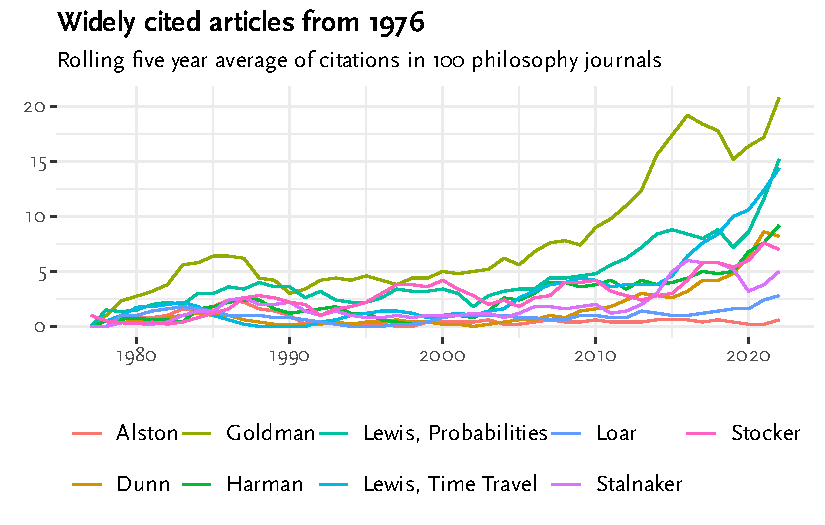
\includegraphics{citations_files/figure-pdf/fig-citation-spaghetti-1976-1.pdf}

}

\caption{\label{fig-citation-spaghetti-1976}Rolling five year average of
citation frequency for widely cited articles from 1976.}

\end{figure}%

\begin{figure}

\centering{

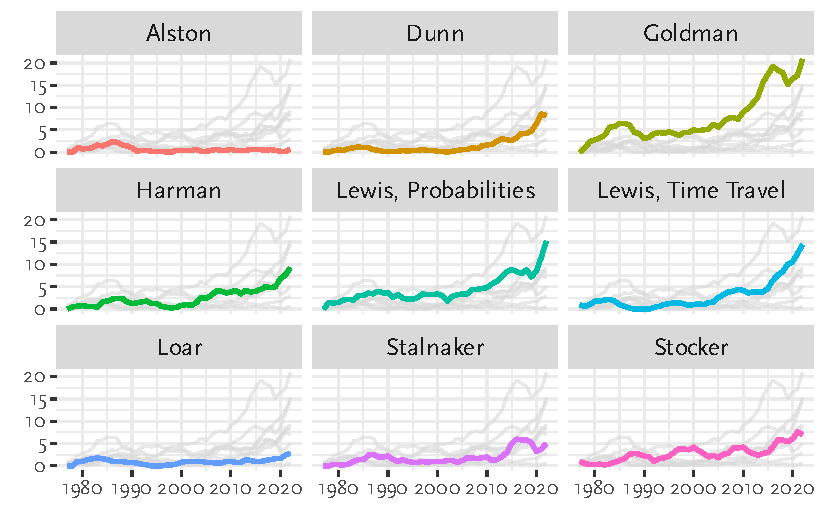
\includegraphics{citations_files/figure-pdf/fig-citation-facet-1976-1.pdf}

}

\caption{\label{fig-citation-facet-1976}Faceted version of
Figure~\ref{fig-citation-spaghetti-1976}.}

\end{figure}%

\newpage

\subsection{1977}\label{sec-s1977}

\subsubsection*{Widely Cited Articles}\label{widely-cited-articles-21}
\addcontentsline{toc}{subsubsection}{Widely Cited Articles}

\begin{enumerate}
\def\labelenumi{\arabic{enumi}.}
\tightlist
\item
  FI Dretske (1977) ``Laws of Nature,'' \emph{Philosophy Of Science}
  44~(2):~248-268.
\item
  SL Darwall (1977) ``Two Kinds of Respect,'' \emph{Ethics}
  88~(1):~36-49.
\item
  J Perry (1977) ``Frege on Demonstratives,'' \emph{Philosophical
  Review} 86~(4):~474-497.
\item
  M Tooley (1977) ``Nature of Laws,'' \emph{Canadian Journal Of
  Philosophy} 7~(4):~667-698.
\item
  JM Taurek (1977) ``Should the Numbers Count?,'' \emph{Philosophy \&
  Public Affairs} 6~(4):~293-316.
\item
  T Burge (1977) ``Belief De Re,'' \emph{Journal Of Philosophy}
  74~(6):~338-362.
\item
  C Boorse (1977) ``Health as a Theoretical Concept,'' \emph{Philosophy
  Of Science} 44~(4):~542-573.
\item
  HH Field (1977) ``Logic, Meaning, and Conceptual Role,'' \emph{Journal
  Of Philosophy} 74~(7):~379-409.
\item
  HN Castañeda (1977) ``Perception, Belief, and Structure of Physical
  Objects and Consciousness,'' \emph{Synthese} 35~(3):~285-351.
\end{enumerate}

\subsubsection*{Citation Count}\label{sec-count-1977}
\addcontentsline{toc}{subsubsection}{Citation Count}

\begin{longtable}[]{@{}lrrr@{}}

\caption{\label{tbl-citation-count-1977}Citation count for widely cited
articles from 1977.}

\tabularnewline

\toprule\noalign{}
Article & All & Early & Late \\
\midrule\noalign{}
\endhead
\bottomrule\noalign{}
\endlastfoot
Dretske & 197 & 22 & 84 \\
Darwall & 190 & 3 & 135 \\
Perry & 189 & 35 & 75 \\
Tooley & 186 & 19 & 85 \\
Taurek & 140 & 10 & 76 \\
Burge & 108 & 34 & 29 \\
Boorse & 103 & 3 & 71 \\
Field & 81 & 23 & 21 \\
Castañeda & 36 & 27 & 1 \\

\end{longtable}

\subsubsection*{Citation Rank}\label{sec-rank-1977}
\addcontentsline{toc}{subsubsection}{Citation Rank}

\begin{longtable}[]{@{}lrrr@{}}

\caption{\label{tbl-citation-rank-1977}Citation rank for widely cited
articles from 1977.}

\tabularnewline

\toprule\noalign{}
Article & Overall & Early & Late \\
\midrule\noalign{}
\endhead
\bottomrule\noalign{}
\endlastfoot
Dretske & 1 & 5 & 3 \\
Darwall & 2 & 84 & 1 \\
Perry & 3 & 1 & 5 \\
Tooley & 4 & 6 & 2 \\
Taurek & 5 & 12 & 4 \\
Burge & 6 & 2 & 10 \\
Boorse & 7 & 84 & 6 \\
Field & 9 & 4 & 15 \\
Castañeda & 19 & 3 & 157 \\

\end{longtable}

\subsubsection*{Citation Trends}\label{sec-trends-1977}
\addcontentsline{toc}{subsubsection}{Citation Trends}

\begin{figure}

\centering{

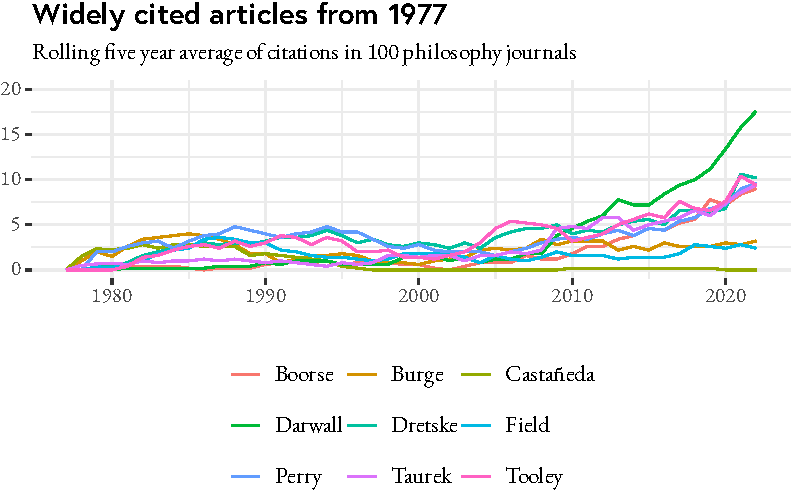
\includegraphics{citations_files/figure-pdf/fig-citation-spaghetti-1977-1.pdf}

}

\caption{\label{fig-citation-spaghetti-1977}Rolling five year average of
citation frequency for widely cited articles from 1977.}

\end{figure}%

\begin{figure}

\centering{

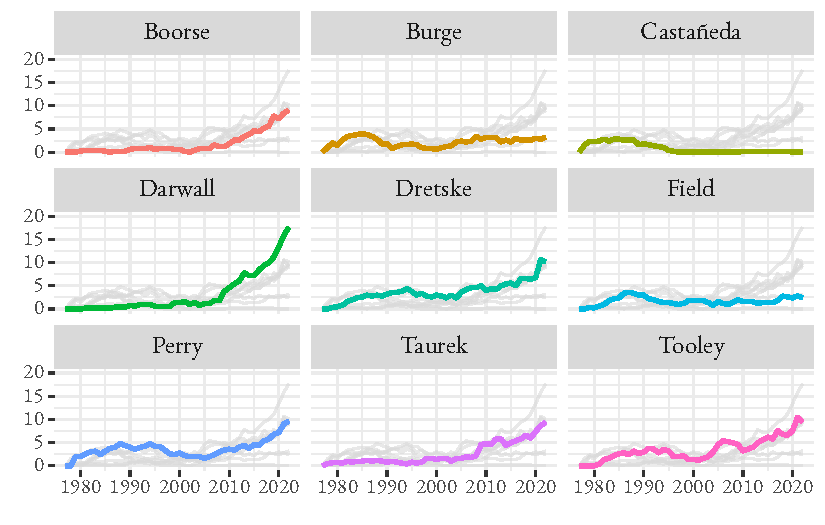
\includegraphics{citations_files/figure-pdf/fig-citation-facet-1977-1.pdf}

}

\caption{\label{fig-citation-facet-1977}Faceted version of
Figure~\ref{fig-citation-spaghetti-1977}.}

\end{figure}%

\newpage

\subsection{1978}\label{sec-s1978}

\subsubsection*{Widely Cited Articles}\label{widely-cited-articles-22}
\addcontentsline{toc}{subsubsection}{Widely Cited Articles}

\begin{enumerate}
\def\labelenumi{\arabic{enumi}.}
\tightlist
\item
  D Lewis (1978) ``Truth in Fiction,'' \emph{American Philosophical
  Quarterly} 15~(1):~37-46.
\item
  DL Hull (1978) ``A Matter of Individuality,'' \emph{Philosophy Of
  Science} 45~(3):~335-360.
\item
  KL Walton (1978) ``Fearing Fictions,'' \emph{Journal Of Philosophy}
  75~(1):~5-27.
\item
  HG Frankfurt (1978) ``The Problem of Action,'' \emph{American
  Philosophical Quarterly} 15~(2):~157-162.
\item
  PR Thagard (1978) ``The Best Explanation: Criteria for Theory
  Choice,'' \emph{Journal Of Philosophy} 75~(2):~76-92.
\item
  J Kim (1978) ``Supervenience and Nomological Incommensurables,''
  \emph{American Philosophical Quarterly} 15~(2):~149-156.
\item
  M Steiner (1978) ``Mathematical Explanation,'' \emph{Philosophical
  Studies} 34~(2):~135-151.
\item
  L BonJour (1978) ``Can Empirical Knowledge Have a Foundation?,''
  \emph{American Philosophical Quarterly} 15~(1):~1-13.
\item
  GS Kavka (1978) ``Some Paradoxes of Deterrence,'' \emph{Journal Of
  Philosophy} 75~(6):~285-302.
\end{enumerate}

\subsubsection*{Citation Count}\label{sec-count-1978}
\addcontentsline{toc}{subsubsection}{Citation Count}

\begin{longtable}[]{@{}lrrr@{}}

\caption{\label{tbl-citation-count-1978}Citation count for widely cited
articles from 1978.}

\tabularnewline

\toprule\noalign{}
Article & All & Early & Late \\
\midrule\noalign{}
\endhead
\bottomrule\noalign{}
\endlastfoot
Lewis & 168 & 19 & 101 \\
Hull & 142 & 17 & 52 \\
Walton & 97 & 22 & 43 \\
Frankfurt & 82 & 7 & 62 \\
Thagard & 80 & 10 & 47 \\
Kim & 76 & 34 & 2 \\
Steiner & 73 & 5 & 47 \\
BonJour & 51 & 17 & 14 \\
Kavka & 42 & 18 & 3 \\

\end{longtable}

\subsubsection*{Citation Rank}\label{sec-rank-1978}
\addcontentsline{toc}{subsubsection}{Citation Rank}

\begin{longtable}[]{@{}lrrr@{}}

\caption{\label{tbl-citation-rank-1978}Citation rank for widely cited
articles from 1978.}

\tabularnewline

\toprule\noalign{}
Article & Overall & Early & Late \\
\midrule\noalign{}
\endhead
\bottomrule\noalign{}
\endlastfoot
Lewis & 1 & 3 & 1 \\
Hull & 2 & 5 & 3 \\
Walton & 3 & 2 & 6 \\
Frankfurt & 4 & 29 & 2 \\
Thagard & 5 & 17 & 4 \\
Kim & 6 & 1 & 92 \\
Steiner & 8 & 44 & 4 \\
BonJour & 13 & 5 & 16 \\
Kavka & 19 & 4 & 70 \\

\end{longtable}

\subsubsection*{Citation Trends}\label{sec-trends-1978}
\addcontentsline{toc}{subsubsection}{Citation Trends}

\begin{figure}

\centering{

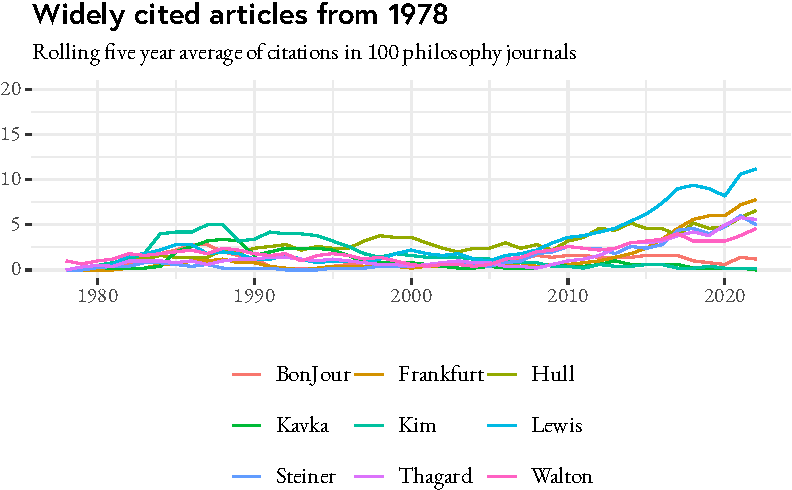
\includegraphics{citations_files/figure-pdf/fig-citation-spaghetti-1978-1.pdf}

}

\caption{\label{fig-citation-spaghetti-1978}Rolling five year average of
citation frequency for widely cited articles from 1978.}

\end{figure}%

\begin{figure}

\centering{

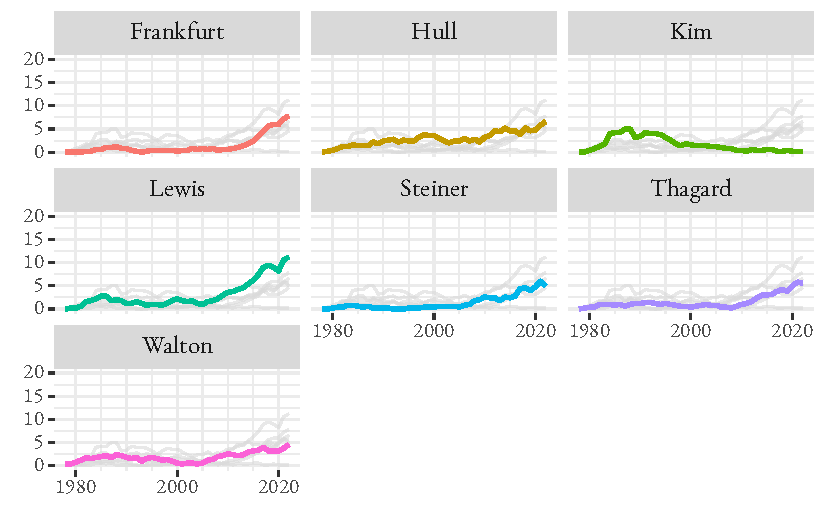
\includegraphics{citations_files/figure-pdf/fig-citation-facet-1978-1.pdf}

}

\caption{\label{fig-citation-facet-1978}Faceted version of
Figure~\ref{fig-citation-spaghetti-1978}.}

\end{figure}%

\newpage

\subsection{1979}\label{sec-s1979}

\subsubsection*{Widely Cited Articles}\label{widely-cited-articles-23}
\addcontentsline{toc}{subsubsection}{Widely Cited Articles}

\begin{enumerate}
\def\labelenumi{\arabic{enumi}.}
\tightlist
\item
  J Perry (1979) ``The Problem of the Essential Indexical,'' \emph{Noûs}
  13~(1):~3-21.
\item
  D Lewis (1979) ``Attitudes De Dicto and De Se,'' \emph{Philosophical
  Review} 88~(4):~513-543.
\item
  D Lewis (1979) ``Counterfactual Dependence and Time's Arrow,''
  \emph{Noûs} 13~(4):~455-476.
\item
  D Lewis (1979) ``Scorekeeping in a Language Game,'' \emph{Journal Of
  Philosophical Logic} 8~(3):~339-359.
\item
  J McDowell (1979) ``Virtue and Reason,'' \emph{Monist}
  62~(3):~331-350.
\item
  G Priest (1979) ``The Logic of Paradox,'' \emph{Journal Of
  Philosophical Logic} 8~(2):~219-241.
\item
  N Daniels (1979) ``Wide Reflective Equilibrium and Theory Acceptance
  in Ethics,'' \emph{Journal Of Philosophy} 76~(5):~256-282.
\item
  RM Adams (1979) ``Primitive Thisness and Primitive Identity,''
  \emph{Journal Of Philosophy} 76~(1):~5-26.
\item
  N Cartwright (1979) ``Causal Laws and Effective Strategies,''
  \emph{Noûs} 13~(4):~419-437.
\end{enumerate}

\subsubsection*{Citation Count}\label{sec-count-1979}
\addcontentsline{toc}{subsubsection}{Citation Count}

\begin{longtable}[]{@{}lrrr@{}}

\caption{\label{tbl-citation-count-1979}Citation count for widely cited
articles from 1979.}

\tabularnewline

\toprule\noalign{}
Article & All & Early & Late \\
\midrule\noalign{}
\endhead
\bottomrule\noalign{}
\endlastfoot
Perry & 393 & 61 & 178 \\
Lewis & 378 & 37 & 229 \\
Lewis & 364 & 37 & 192 \\
Lewis & 347 & 15 & 206 \\
McDowell & 216 & 12 & 90 \\
Priest & 211 & 16 & 146 \\
Daniels & 143 & 40 & 53 \\
Adams & 132 & 25 & 63 \\
Cartwright & 128 & 29 & 49 \\

\end{longtable}

\subsubsection*{Citation Rank}\label{sec-rank-1979}
\addcontentsline{toc}{subsubsection}{Citation Rank}

\begin{longtable}[]{@{}lrrr@{}}

\caption{\label{tbl-citation-rank-1979}Citation rank for widely cited
articles from 1979.}

\tabularnewline

\toprule\noalign{}
Article & Overall & Early & Late \\
\midrule\noalign{}
\endhead
\bottomrule\noalign{}
\endlastfoot
Perry & 1 & 1 & 4 \\
Lewis & 2 & 3 & 1 \\
Lewis & 3 & 3 & 3 \\
Lewis & 4 & 12 & 2 \\
McDowell & 5 & 16 & 6 \\
Priest & 6 & 10 & 5 \\
Daniels & 7 & 2 & 9 \\
Adams & 8 & 6 & 8 \\
Cartwright & 9 & 5 & 10 \\

\end{longtable}

\subsubsection*{Citation Trends}\label{sec-trends-1979}
\addcontentsline{toc}{subsubsection}{Citation Trends}

\begin{figure}

\centering{

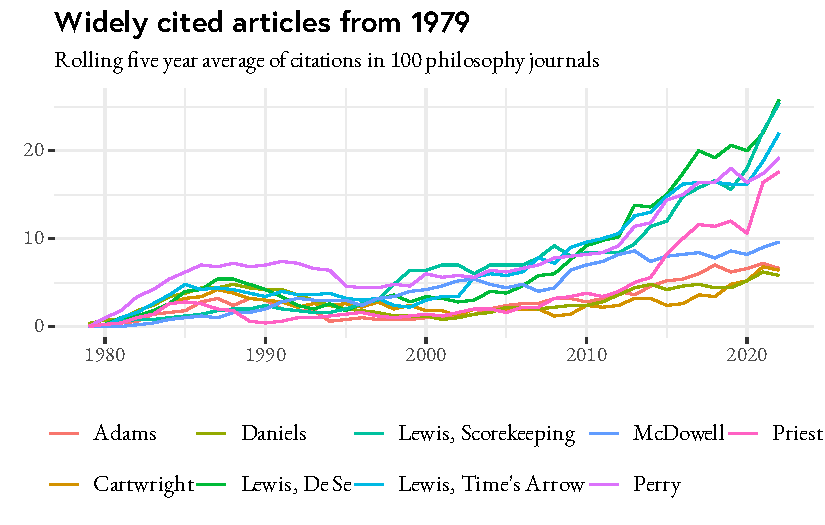
\includegraphics{citations_files/figure-pdf/fig-citation-spaghetti-1979-1.pdf}

}

\caption{\label{fig-citation-spaghetti-1979}Rolling five year average of
citation frequency for widely cited articles from 1979.}

\end{figure}%

\begin{figure}

\centering{

\includegraphics{citations_files/figure-pdf/fig-citation-facet-1979-1.pdf}

}

\caption{\label{fig-citation-facet-1979}Faceted version of
Figure~\ref{fig-citation-spaghetti-1979}.}

\end{figure}%

\newpage

\subsection{1980}\label{sec-s1980}

\subsubsection*{Widely Cited Articles}\label{widely-cited-articles-24}
\addcontentsline{toc}{subsubsection}{Widely Cited Articles}

\begin{enumerate}
\def\labelenumi{\arabic{enumi}.}
\tightlist
\item
  J Rawls (1980) ``Rational and Full Autonomy,'' \emph{Journal Of
  Philosophy} 77~(9):~515-535.
\item
  M Davies and L Humberstone (1980) ``Two Notions of Necessity,''
  \emph{Philosophical Studies} 38~(1):~1-30.
\item
  J Levinson (1980) ``What a Musical Work Is,'' \emph{Journal Of
  Philosophy} 77~(1):~5-28.
\item
  E Sober (1980) ``Evolution, Population Thinking, and Essentialism,''
  \emph{Philosophy Of Science} 47~(3):~350-383.
\item
  RB Marcus (1980) ``Moral Dilemmas and Consistency,'' \emph{Journal Of
  Philosophy} 77~(3):~121-136.
\item
  D Lewis (1980) ``Veridical Hallucination and Prosthetic Vision,''
  \emph{Australasian Journal Of Philosophy} 58~(3):~239-249.
\item
  N Daniels (1980) ``Reflective Equilibrium and Archimedean Points,''
  \emph{Canadian Journal Of Philosophy} 10~(1):~83-103.
\item
  N Block (1980) ``Are Absent Qualia Impossible,'' \emph{Philosophical
  Review} 89~(2):~257-274.
\end{enumerate}

\subsubsection*{Citation Count}\label{sec-count-1980}
\addcontentsline{toc}{subsubsection}{Citation Count}

\begin{longtable}[]{@{}lrrr@{}}

\caption{\label{tbl-citation-count-1980}Citation count for widely cited
articles from 1980.}

\tabularnewline

\toprule\noalign{}
Article & All & Early & Late \\
\midrule\noalign{}
\endhead
\bottomrule\noalign{}
\endlastfoot
Rawls & 188 & 52 & 58 \\
Davies and Humberstone & 121 & 3 & 61 \\
Levinson & 100 & 10 & 55 \\
Sober & 89 & 9 & 40 \\
Marcus & 82 & 24 & 35 \\
Lewis & 81 & 10 & 45 \\
Daniels & 41 & 22 & 8 \\
Block & 38 & 19 & 4 \\

\end{longtable}

\subsubsection*{Citation Rank}\label{sec-rank-1980}
\addcontentsline{toc}{subsubsection}{Citation Rank}

\begin{longtable}[]{@{}lrrr@{}}

\caption{\label{tbl-citation-rank-1980}Citation rank for widely cited
articles from 1980.}

\tabularnewline

\toprule\noalign{}
Article & Overall & Early & Late \\
\midrule\noalign{}
\endhead
\bottomrule\noalign{}
\endlastfoot
Rawls & 1 & 1 & 2 \\
Davies and Humberstone & 2 & 94 & 1 \\
Levinson & 3 & 10 & 3 \\
Sober & 4 & 14 & 5 \\
Marcus & 5 & 2 & 6 \\
Lewis & 6 & 10 & 4 \\
Daniels & 8 & 3 & 29 \\
Block & 11 & 4 & 67 \\

\end{longtable}

\subsubsection*{Citation Trends}\label{sec-trends-1980}
\addcontentsline{toc}{subsubsection}{Citation Trends}

\begin{figure}

\centering{

\includegraphics{citations_files/figure-pdf/fig-citation-spaghetti-1980-1.pdf}

}

\caption{\label{fig-citation-spaghetti-1980}Rolling five year average of
citation frequency for widely cited articles from 1980.}

\end{figure}%

\begin{figure}

\centering{

\includegraphics{citations_files/figure-pdf/fig-citation-facet-1980-1.pdf}

}

\caption{\label{fig-citation-facet-1980}Faceted version of
Figure~\ref{fig-citation-spaghetti-1980}.}

\end{figure}%

\newpage

\subsection{1981}\label{sec-s1981}

\subsubsection*{Widely Cited Articles}\label{widely-cited-articles-25}
\addcontentsline{toc}{subsubsection}{Widely Cited Articles}

\begin{enumerate}
\def\labelenumi{\arabic{enumi}.}
\tightlist
\item
  L Laudan (1981) ``A Confutation of Convergent Realism,''
  \emph{Philosophy Of Science} 48~(1):~19-49.
\item
  P Kitcher (1981) ``Explanatory Unification,'' \emph{Philosophy Of
  Science} 48~(4):~507-531.
\item
  PM Churchland (1981) ``Eliminative Materialism and the Propositional
  Attitudes,'' \emph{Journal Of Philosophy} 78~(2):~67-90.
\item
  R Dworkin (1981) ``What is Equality? Part 2: Equality of Resources,''
  \emph{Philosophy \& Public Affairs} 10~(4):~283-345.
\item
  D Lewis (1981) ``Causal Decision Theory,'' \emph{Australasian Journal
  Of Philosophy} 59~(1):~5-30.
\item
  P van Inwagen (1981) ``The Doctrine of Arbitrary Undetached Parts,''
  \emph{Pacific Philosophical Quarterly} 62~(2):~123-137.
\item
  J Dupre (1981) ``Natural Kinds and Biological Taxa,''
  \emph{Philosophical Review} 90~(1):~66-90.
\item
  RM Adams (1981) ``Actualism and Thisness,'' \emph{Synthese}
  49~(1):~3-41.
\item
  R Dworkin (1981) ``What is Equality? Part 1: Equality of Welfare,''
  \emph{Philosophy \& Public Affairs} 10~(3):~185-246.
\end{enumerate}

\subsubsection*{Citation Count}\label{sec-count-1981}
\addcontentsline{toc}{subsubsection}{Citation Count}

\begin{longtable}[]{@{}lrrr@{}}

\caption{\label{tbl-citation-count-1981}Citation count for widely cited
articles from 1981.}

\tabularnewline

\toprule\noalign{}
Article & All & Early & Late \\
\midrule\noalign{}
\endhead
\bottomrule\noalign{}
\endlastfoot
Laudan & 271 & 28 & 139 \\
Kitcher & 239 & 10 & 134 \\
Churchland & 236 & 58 & 105 \\
Dworkin Pt. 2 & 174 & 22 & 68 \\
Lewis & 160 & 32 & 95 \\
van Inwagen & 106 & 6 & 35 \\
Dupre & 88 & 16 & 24 \\
Adams & 85 & 13 & 48 \\
Dworkin Pt. 1 & 77 & 16 & 22 \\

\end{longtable}

\subsubsection*{Citation Rank}\label{sec-rank-1981}
\addcontentsline{toc}{subsubsection}{Citation Rank}

\begin{longtable}[]{@{}lrrr@{}}

\caption{\label{tbl-citation-rank-1981}Citation rank for widely cited
articles from 1981.}

\tabularnewline

\toprule\noalign{}
Article & Overall & Early & Late \\
\midrule\noalign{}
\endhead
\bottomrule\noalign{}
\endlastfoot
Laudan & 1 & 3 & 1 \\
Kitcher & 2 & 14 & 2 \\
Churchland & 3 & 1 & 3 \\
Dworkin Pt. 2 & 4 & 4 & 5 \\
Lewis & 5 & 2 & 4 \\
van Inwagen & 6 & 39 & 9 \\
Dupre & 8 & 5 & 15 \\
Adams & 9 & 9 & 6 \\
Dworkin Pt. 1 & 11 & 5 & 20 \\

\end{longtable}

\subsubsection*{Citation Trends}\label{sec-trends-1981}
\addcontentsline{toc}{subsubsection}{Citation Trends}

\begin{figure}

\centering{

\includegraphics{citations_files/figure-pdf/fig-citation-spaghetti-1981-1.pdf}

}

\caption{\label{fig-citation-spaghetti-1981}Rolling five year average of
citation frequency for widely cited articles from 1981.}

\end{figure}%

\begin{figure}

\centering{

\includegraphics{citations_files/figure-pdf/fig-citation-facet-1981-1.pdf}

}

\caption{\label{fig-citation-facet-1981}Faceted version of
Figure~\ref{fig-citation-spaghetti-1981}.}

\end{figure}%

\newpage

\subsection{1982}\label{sec-s1982}

\subsubsection*{Widely Cited Articles}\label{widely-cited-articles-26}
\addcontentsline{toc}{subsubsection}{Widely Cited Articles}

\begin{enumerate}
\def\labelenumi{\arabic{enumi}.}
\tightlist
\item
  F Jackson (1982) ``Epiphenomenal Qualia,'' \emph{Philosophical
  Quarterly} 32~(127):~127-136.
\item
  S Wolf (1982) ``Moral Saints,'' \emph{Journal Of Philosophy}
  79~(8):~419-439.
\item
  EW Prior, R Pargetter, and F Jackson (1982) ``Three Theses About
  Dispositions,'' \emph{American Philosophical Quarterly}
  19~(3):~251-257.
\item
  C Swoyer (1982) ``The Nature of Natural Laws,'' \emph{Australasian
  Journal Of Philosophy} 60~(3):~203-223.
\item
  D Lewis (1982) ``Logic for Equivocators,'' \emph{Noûs}
  16~(3):~431-441.
\item
  A Gupta (1982) ``Truth and Paradox,'' \emph{Journal Of Philosophical
  Logic} 11~(1):~1-60.
\item
  J Kim (1982) ``Psychophysical Supervenience,'' \emph{Philosophical
  Studies} 41~(1):~51-70.
\item
  D Shapere (1982) ``The Concept of Observation in Science and
  Philosophy,'' \emph{Philosophy Of Science} 49~(4):~485-525.
\item
  J Haugeland (1982) ``Weak Supervenience,'' \emph{American
  Philosophical Quarterly} 19~(1):~93-103.
\end{enumerate}

\subsubsection*{Citation Count}\label{sec-count-1982}
\addcontentsline{toc}{subsubsection}{Citation Count}

\begin{longtable}[]{@{}lrrr@{}}

\caption{\label{tbl-citation-count-1982}Citation count for widely cited
articles from 1982.}

\tabularnewline

\toprule\noalign{}
Article & All & Early & Late \\
\midrule\noalign{}
\endhead
\bottomrule\noalign{}
\endlastfoot
Jackson & 449 & 26 & 227 \\
Wolf & 152 & 17 & 68 \\
Prior et al & 129 & 10 & 62 \\
Swoyer & 109 & 9 & 46 \\
Lewis & 87 & 3 & 73 \\
Gupta & 85 & 23 & 39 \\
Kim & 80 & 23 & 17 \\
Shapere & 47 & 21 & 10 \\
Haugeland & 43 & 26 & 3 \\

\end{longtable}

\subsubsection*{Citation Rank}\label{sec-rank-1982}
\addcontentsline{toc}{subsubsection}{Citation Rank}

\begin{longtable}[]{@{}lrrr@{}}

\caption{\label{tbl-citation-rank-1982}Citation rank for widely cited
articles from 1982.}

\tabularnewline

\toprule\noalign{}
Article & Overall & Early & Late \\
\midrule\noalign{}
\endhead
\bottomrule\noalign{}
\endlastfoot
Jackson & 1 & 1 & 1 \\
Wolf & 2 & 7 & 3 \\
Prior et al & 3 & 19 & 4 \\
Swoyer & 4 & 24 & 5 \\
Lewis & 5 & 111 & 2 \\
Gupta & 6 & 3 & 7 \\
Kim & 7 & 3 & 19 \\
Shapere & 15 & 5 & 36 \\
Haugeland & 20 & 1 & 115 \\

\end{longtable}

\subsubsection*{Citation Trends}\label{sec-trends-1982}
\addcontentsline{toc}{subsubsection}{Citation Trends}

\begin{figure}

\centering{

\includegraphics{citations_files/figure-pdf/fig-citation-spaghetti-1982-1.pdf}

}

\caption{\label{fig-citation-spaghetti-1982}Rolling five year average of
citation frequency for widely cited articles from 1982.}

\end{figure}%

\begin{figure}

\centering{

\includegraphics{citations_files/figure-pdf/fig-citation-facet-1982-1.pdf}

}

\caption{\label{fig-citation-facet-1982}Faceted version of
Figure~\ref{fig-citation-spaghetti-1982}.}

\end{figure}%

\newpage

\subsection{1983}\label{sec-s1983}

\subsubsection*{Widely Cited Articles}\label{widely-cited-articles-27}
\addcontentsline{toc}{subsubsection}{Widely Cited Articles}

\begin{enumerate}
\def\labelenumi{\arabic{enumi}.}
\tightlist
\item
  D Lewis (1983) ``New Work for a Theory of Universals,''
  \emph{Australasian Journal Of Philosophy} 61~(4):~343-377.
\item
  J Levine (1983) ``Materialism and Qualia: The Explanatory Gap,''
  \emph{Pacific Philosophical Quarterly} 64~(4):~354-361.
\item
  GS Kavka (1983) ``The Toxin Puzzle,'' \emph{Analysis} 43~(1):~33-36.
\item
  CM Korsgaard (1983) ``Two Distinctions in Goodness,''
  \emph{Philosophical Review} 92~(2):~169-195.
\item
  R Brandom (1983) ``Asserting,'' \emph{Noûs} 17~(4):~637-650.
\item
  H Kornblith (1983) ``Justified Belief and Epistemically Responsible
  Action,'' \emph{Philosophical Review} 92~(1):~33-48.
\item
  E Eells and E Sober (1983) ``Probabilistic Causality and the Question
  of Transitivity,'' \emph{Philosophy Of Science} 50~(1):~35-57.
\item
  P Foot (1983) ``Moral Realism and Moral Dilemma,'' \emph{Journal Of
  Philosophy} 80~(7):~379-398.
\end{enumerate}

\subsubsection*{Citation Count}\label{sec-count-1983}
\addcontentsline{toc}{subsubsection}{Citation Count}

\begin{longtable}[]{@{}lrrr@{}}

\caption{\label{tbl-citation-count-1983}Citation count for widely cited
articles from 1983.}

\tabularnewline

\toprule\noalign{}
Article & All & Early & Late \\
\midrule\noalign{}
\endhead
\bottomrule\noalign{}
\endlastfoot
Lewis & 755 & 46 & 515 \\
Levine & 207 & 2 & 107 \\
Kavka & 163 & 15 & 85 \\
Korsgaard & 134 & 5 & 88 \\
Brandom & 96 & 7 & 57 \\
Kornblith & 80 & 21 & 39 \\
Eells and Sober & 40 & 20 & 5 \\
Foot & 38 & 14 & 10 \\

\end{longtable}

\subsubsection*{Citation Rank}\label{sec-rank-1983}
\addcontentsline{toc}{subsubsection}{Citation Rank}

\begin{longtable}[]{@{}lrrr@{}}

\caption{\label{tbl-citation-rank-1983}Citation rank for widely cited
articles from 1983.}

\tabularnewline

\toprule\noalign{}
Article & Overall & Early & Late \\
\midrule\noalign{}
\endhead
\bottomrule\noalign{}
\endlastfoot
Lewis & 1 & 1 & 1 \\
Levine & 2 & 177 & 2 \\
Kavka & 3 & 4 & 4 \\
Korsgaard & 4 & 49 & 3 \\
Brandom & 5 & 26 & 5 \\
Kornblith & 9 & 2 & 10 \\
Eells and Sober & 14 & 3 & 63 \\
Foot & 15 & 5 & 33 \\

\end{longtable}

\subsubsection*{Citation Trends}\label{sec-trends-1983}
\addcontentsline{toc}{subsubsection}{Citation Trends}

\begin{figure}

\centering{

\includegraphics{citations_files/figure-pdf/fig-citation-spaghetti-1983-1.pdf}

}

\caption{\label{fig-citation-spaghetti-1983}Rolling five year average of
citation frequency for widely cited articles from 1983.}

\end{figure}%

\begin{figure}

\centering{

\includegraphics{citations_files/figure-pdf/fig-citation-facet-1983-1.pdf}

}

\caption{\label{fig-citation-facet-1983}Faceted version of
Figure~\ref{fig-citation-spaghetti-1983}.}

\end{figure}%

\newpage

\subsection{1984}\label{sec-s1984}

\subsubsection*{Widely Cited Articles}\label{widely-cited-articles-28}
\addcontentsline{toc}{subsubsection}{Widely Cited Articles}

\begin{enumerate}
\def\labelenumi{\arabic{enumi}.}
\tightlist
\item
  D Lewis (1984) ``Putnam's Paradox,'' \emph{Australasian Journal Of
  Philosophy} 62~(3):~221-236.
\item
  BC van Fraassen (1984) ``Belief and the Will,'' \emph{Journal Of
  Philosophy} 81~(5):~235-256.
\item
  P Railton (1984) ``Alienation, Consequentialism, and the Demands of
  Morality,'' \emph{Philosophy \& Public Affairs} 13~(2):~134-171.
\item
  G Boolos (1984) ``To Be is To Be a Value of a Variable (Or To Be Some
  Values of Some Variables),'' \emph{Journal Of Philosophy}
  81~(8):~430-449.
\item
  J Kim (1984) ``Concepts of Supervenience,'' \emph{Philosophy And
  Phenomenological Research} 45~(2):~153-176.
\item
  S Cohen (1984) ``Justification and Truth,'' \emph{Philosophical
  Studies} 46~(3):~279-295.
\item
  P Kitcher (1984) ``Species,'' \emph{Philosophy Of Science}
  51~(2):~308-333.
\item
  J Fodor (1984) ``Observation Reconsidered,'' \emph{Philosophy Of
  Science} 51~(1):~23-43.
\item
  J Kim (1984) ``Epiphenomenal and Supervenient Causation,''
  \emph{Midwest Studies In Philosophy} 9:~257-270.
\end{enumerate}

\subsubsection*{Citation Count}\label{sec-count-1984}
\addcontentsline{toc}{subsubsection}{Citation Count}

\begin{longtable}[]{@{}lrrr@{}}

\caption{\label{tbl-citation-count-1984}Citation count for widely cited
articles from 1984.}

\tabularnewline

\toprule\noalign{}
Article & All & Early & Late \\
\midrule\noalign{}
\endhead
\bottomrule\noalign{}
\endlastfoot
Lewis & 229 & 20 & 129 \\
van Fraassen & 205 & 19 & 101 \\
Railton & 198 & 19 & 112 \\
Boolos & 183 & 12 & 104 \\
Kim & 154 & 50 & 34 \\
Cohen & 149 & 10 & 100 \\
Kitcher & 113 & 20 & 44 \\
Fodor & 82 & 21 & 34 \\
Kim & 61 & 20 & 10 \\

\end{longtable}

\subsubsection*{Citation Rank}\label{sec-rank-1984}
\addcontentsline{toc}{subsubsection}{Citation Rank}

\begin{longtable}[]{@{}lrrr@{}}

\caption{\label{tbl-citation-rank-1984}Citation rank for widely cited
articles from 1984.}

\tabularnewline

\toprule\noalign{}
Article & Overall & Early & Late \\
\midrule\noalign{}
\endhead
\bottomrule\noalign{}
\endlastfoot
Lewis & 1 & 3 & 1 \\
van Fraassen & 2 & 6 & 4 \\
Railton & 3 & 6 & 2 \\
Boolos & 4 & 14 & 3 \\
Kim & 5 & 1 & 10 \\
Cohen & 6 & 20 & 5 \\
Kitcher & 7 & 3 & 8 \\
Fodor & 10 & 2 & 10 \\
Kim & 13 & 3 & 47 \\

\end{longtable}

\subsubsection*{Citation Trends}\label{sec-trends-1984}
\addcontentsline{toc}{subsubsection}{Citation Trends}

\begin{figure}

\centering{

\includegraphics{citations_files/figure-pdf/fig-citation-spaghetti-1984-1.pdf}

}

\caption{\label{fig-citation-spaghetti-1984}Rolling five year average of
citation frequency for widely cited articles from 1984.}

\end{figure}%

\begin{figure}

\centering{

\includegraphics{citations_files/figure-pdf/fig-citation-facet-1984-1.pdf}

}

\caption{\label{fig-citation-facet-1984}Faceted version of
Figure~\ref{fig-citation-spaghetti-1984}.}

\end{figure}%

\newpage

\subsection{1985}\label{sec-s1985}

\subsubsection*{Widely Cited Articles}\label{widely-cited-articles-29}
\addcontentsline{toc}{subsubsection}{Widely Cited Articles}

\begin{enumerate}
\def\labelenumi{\arabic{enumi}.}
\tightlist
\item
  R Feldman and E Conee (1985) ``Evidentialism,'' \emph{Philosophical
  Studies} 48~(1):~15-34.
\item
  E McMullin (1985) ``Galilean Idealization,'' \emph{Studies In History
  And Philosophy Of Science} 16~(3):~247-273.
\item
  J Hardwig (1985) ``Epistemic Dependence,'' \emph{Journal Of
  Philosophy} 82~(7):~335-349.
\item
  V McGee (1985) ``A Counterexample To Modus Ponens,'' \emph{Journal Of
  Philosophy} 82~(9):~462-471.
\item
  G Boolos (1985) ``Nominalist Platonism,'' \emph{Philosophical Review}
  94~(3):~327-344.
\item
  J Rawls (1985) ``Justice as Fairness: Political Not Metaphysical,''
  \emph{Philosophy \& Public Affairs} 14~(3):~223-251.
\item
  WP Alston (1985) ``Concepts of Epistemic Justification,''
  \emph{Monist} 68~(1):~57-89.
\item
  RM Adams (1985) ``Involuntary Sins,'' \emph{Philosophical Review}
  94~(1):~3-31.
\item
  R Feldman (1985) ``Reliability and Justification,'' \emph{Monist}
  68~(2):~159-174.
\end{enumerate}

\subsubsection*{Citation Count}\label{sec-count-1985}
\addcontentsline{toc}{subsubsection}{Citation Count}

\begin{longtable}[]{@{}lrrr@{}}

\caption{\label{tbl-citation-count-1985}Citation count for widely cited
articles from 1985.}

\tabularnewline

\toprule\noalign{}
Article & All & Early & Late \\
\midrule\noalign{}
\endhead
\bottomrule\noalign{}
\endlastfoot
Feldman and Conee & 171 & 6 & 118 \\
McMullin & 141 & 5 & 89 \\
Hardwig & 135 & 10 & 84 \\
McGee & 126 & 7 & 93 \\
Boolos & 97 & 9 & 43 \\
Rawls & 89 & 42 & 22 \\
Alston & 88 & 18 & 40 \\
Adams & 77 & 4 & 53 \\
Feldman & 76 & 19 & 28 \\

\end{longtable}

\subsubsection*{Citation Rank}\label{sec-rank-1985}
\addcontentsline{toc}{subsubsection}{Citation Rank}

\begin{longtable}[]{@{}lrrr@{}}

\caption{\label{tbl-citation-rank-1985}Citation rank for widely cited
articles from 1985.}

\tabularnewline

\toprule\noalign{}
Article & Overall & Early & Late \\
\midrule\noalign{}
\endhead
\bottomrule\noalign{}
\endlastfoot
Feldman and Conee & 1 & 30 & 1 \\
McMullin & 2 & 50 & 3 \\
Hardwig & 3 & 7 & 4 \\
McGee & 4 & 21 & 2 \\
Boolos & 5 & 10 & 6 \\
Rawls & 6 & 1 & 11 \\
Alston & 7 & 4 & 7 \\
Adams & 8 & 68 & 5 \\
Feldman & 9 & 3 & 9 \\

\end{longtable}

\subsubsection*{Citation Trends}\label{sec-trends-1985}
\addcontentsline{toc}{subsubsection}{Citation Trends}

\begin{figure}

\centering{

\includegraphics{citations_files/figure-pdf/fig-citation-spaghetti-1985-1.pdf}

}

\caption{\label{fig-citation-spaghetti-1985}Rolling five year average of
citation frequency for widely cited articles from 1985.}

\end{figure}%

\begin{figure}

\centering{

\includegraphics{citations_files/figure-pdf/fig-citation-facet-1985-1.pdf}

}

\caption{\label{fig-citation-facet-1985}Faceted version of
Figure~\ref{fig-citation-spaghetti-1985}.}

\end{figure}%

\newpage

\subsection{1986}\label{sec-s1986}

\subsubsection*{Widely Cited Articles}\label{widely-cited-articles-30}
\addcontentsline{toc}{subsubsection}{Widely Cited Articles}

\begin{enumerate}
\def\labelenumi{\arabic{enumi}.}
\tightlist
\item
  P Railton (1986) ``Moral Realism,'' \emph{Philosophical Review}
  95~(2):~163-207.
\item
  T Burge (1986) ``Individualism and Psychology,'' \emph{Philosophical
  Review} 95~(1):~3-45.
\item
  CM Korsgaard (1986) ``Skepticism About Practical Reason,''
  \emph{Journal Of Philosophy} 83~(1):~5-25.
\item
  A Baier (1986) ``Trust and Antitrust,'' \emph{Ethics} 96~(2):~231-260.
\item
  DM Rosenthal (1986) ``Two Concepts of Consciousness,''
  \emph{Philosophical Studies} 49~(3):~329-359.
\item
  N Block (1986) ``Advertisement for a Semantics for Psychology,''
  \emph{Midwest Studies In Philosophy} 10:~615-678.
\item
  F Jackson and R Pargetter (1986) ``Oughts, Options, and Actualism,''
  \emph{Philosophical Review} 95~(2):~233-255.
\item
  RG Millikan (1986) ``Thoughts Without Laws, Cognitive Science With
  Content,'' \emph{Philosophical Review} 95~(1):~47-80.
\end{enumerate}

\subsubsection*{Citation Count}\label{sec-count-1986}
\addcontentsline{toc}{subsubsection}{Citation Count}

\begin{longtable}[]{@{}lrrr@{}}

\caption{\label{tbl-citation-count-1986}Citation count for widely cited
articles from 1986.}

\tabularnewline

\toprule\noalign{}
Article & All & Early & Late \\
\midrule\noalign{}
\endhead
\bottomrule\noalign{}
\endlastfoot
Railton & 230 & 39 & 111 \\
Burge & 164 & 53 & 48 \\
Korsgaard & 150 & 15 & 70 \\
Baier & 138 & 23 & 87 \\
Rosenthal & 112 & 9 & 44 \\
Block & 109 & 18 & 49 \\
Jackson and Pargetter & 99 & 10 & 66 \\
Millikan & 39 & 22 & 3 \\

\end{longtable}

\subsubsection*{Citation Rank}\label{sec-rank-1986}
\addcontentsline{toc}{subsubsection}{Citation Rank}

\begin{longtable}[]{@{}lrrr@{}}

\caption{\label{tbl-citation-rank-1986}Citation rank for widely cited
articles from 1986.}

\tabularnewline

\toprule\noalign{}
Article & Overall & Early & Late \\
\midrule\noalign{}
\endhead
\bottomrule\noalign{}
\endlastfoot
Railton & 1 & 2 & 1 \\
Burge & 2 & 1 & 6 \\
Korsgaard & 3 & 8 & 3 \\
Baier & 4 & 3 & 2 \\
Rosenthal & 5 & 25 & 8 \\
Block & 6 & 5 & 5 \\
Jackson and Pargetter & 7 & 17 & 4 \\
Millikan & 24 & 4 & 133 \\

\end{longtable}

\subsubsection*{Citation Trends}\label{sec-trends-1986}
\addcontentsline{toc}{subsubsection}{Citation Trends}

\begin{figure}

\centering{

\includegraphics{citations_files/figure-pdf/fig-citation-spaghetti-1986-1.pdf}

}

\caption{\label{fig-citation-spaghetti-1986}Rolling five year average of
citation frequency for widely cited articles from 1986.}

\end{figure}%

\begin{figure}

\centering{

\includegraphics{citations_files/figure-pdf/fig-citation-facet-1986-1.pdf}

}

\caption{\label{fig-citation-facet-1986}Faceted version of
Figure~\ref{fig-citation-spaghetti-1986}.}

\end{figure}%

\newpage

\subsection{1987}\label{sec-s1987}

\subsubsection*{Widely Cited Articles}\label{widely-cited-articles-31}
\addcontentsline{toc}{subsubsection}{Widely Cited Articles}

\begin{enumerate}
\def\labelenumi{\arabic{enumi}.}
\tightlist
\item
  M Smith (1987) ``The Humean Theory of Motivation,'' \emph{Mind}
  96~(381):~36-61.
\item
  J Bigelow and R Pargetter (1987) ``Functions,'' \emph{Journal Of
  Philosophy} 84~(4):~181-196.
\item
  H Frankfurt (1987) ``Equality as a Moral Ideal,'' \emph{Ethics}
  98~(1):~21-43.
\item
  J Earman and J Norton (1987) ``What Price Spacetime Substantivalism:
  The Hole Story,'' \emph{British Journal For The Philosophy Of Science}
  38~(4):~515-525.
\item
  DW Stampe (1987) ``The Authority of Desire,'' \emph{Philosophical
  Review} 96~(3):~335-381.
\item
  LS Temkin (1987) ``Intransitivity and the Mere Addition Paradox,''
  \emph{Philosophy \& Public Affairs} 16~(2):~138-187.
\item
  T Nagel (1987) ``Moral Conflict and Political Legitimacy,''
  \emph{Philosophy \& Public Affairs} 16~(3):~215-240.
\item
  M Gilbert (1987) ``Modeling Collective Belief,'' \emph{Synthese}
  73~(1):~185-204.
\item
  L Laudan (1987) ``Progress or Rationality: The Prospects for Normative
  Naturalism,'' \emph{American Philosophical Quarterly} 24~(1):~19-31.
\end{enumerate}

\subsubsection*{Citation Count}\label{sec-count-1987}
\addcontentsline{toc}{subsubsection}{Citation Count}

\begin{longtable}[]{@{}lrrr@{}}

\caption{\label{tbl-citation-count-1987}Citation count for widely cited
articles from 1987.}

\tabularnewline

\toprule\noalign{}
Article & All & Early & Late \\
\midrule\noalign{}
\endhead
\bottomrule\noalign{}
\endlastfoot
Smith & 120 & 19 & 61 \\
Bigelow and Pargetter & 89 & 23 & 33 \\
Frankfurt & 89 & 1 & 60 \\
Earman and Norton & 81 & 20 & 36 \\
Stampe & 78 & 6 & 53 \\
Temkin & 68 & 3 & 41 \\
Nagel & 67 & 17 & 24 \\
Gilbert & 62 & 5 & 46 \\
Laudan & 52 & 27 & 10 \\

\end{longtable}

\subsubsection*{Citation Rank}\label{sec-rank-1987}
\addcontentsline{toc}{subsubsection}{Citation Rank}

\begin{longtable}[]{@{}lrrr@{}}

\caption{\label{tbl-citation-rank-1987}Citation rank for widely cited
articles from 1987.}

\tabularnewline

\toprule\noalign{}
Article & Overall & Early & Late \\
\midrule\noalign{}
\endhead
\bottomrule\noalign{}
\endlastfoot
Smith & 1 & 4 & 1 \\
Bigelow and Pargetter & 2 & 2 & 7 \\
Frankfurt & 2 & 253 & 2 \\
Earman and Norton & 4 & 3 & 6 \\
Stampe & 5 & 31 & 3 \\
Temkin & 7 & 91 & 5 \\
Nagel & 8 & 5 & 12 \\
Gilbert & 9 & 42 & 4 \\
Laudan & 13 & 1 & 35 \\

\end{longtable}

\subsubsection*{Citation Trends}\label{sec-trends-1987}
\addcontentsline{toc}{subsubsection}{Citation Trends}

\begin{figure}

\centering{

\includegraphics{citations_files/figure-pdf/fig-citation-spaghetti-1987-1.pdf}

}

\caption{\label{fig-citation-spaghetti-1987}Rolling five year average of
citation frequency for widely cited articles from 1987.}

\end{figure}%

\begin{figure}

\centering{

\includegraphics{citations_files/figure-pdf/fig-citation-facet-1987-1.pdf}

}

\caption{\label{fig-citation-facet-1987}Faceted version of
Figure~\ref{fig-citation-spaghetti-1987}.}

\end{figure}%

\newpage

\subsection{1988}\label{sec-s1988}

\subsubsection*{Widely Cited Articles}\label{widely-cited-articles-32}
\addcontentsline{toc}{subsubsection}{Widely Cited Articles}

\begin{enumerate}
\def\labelenumi{\arabic{enumi}.}
\tightlist
\item
  T Burge (1988) ``Individualism and Self-Knowledge,'' \emph{Journal Of
  Philosophy} 85~(11):~649-663.
\item
  J Bogen and J Woodward (1988) ``Saving the Phenomena,''
  \emph{Philosophical Review} 97~(3):~303-352.
\item
  A Grove (1988) ``Two Modelings for Theory Change,'' \emph{Journal Of
  Philosophical Logic} 17~(2):~157-170.
\item
  K Sterelny and P Kitcher (1988) ``The Return of the Gene,''
  \emph{Journal Of Philosophy} 85~(7):~339-361.
\item
  S Kagan (1988) ``The Additive Fallacy,'' \emph{Ethics} 99~(1):~5-31.
\item
  WP Alston (1988) ``An Internalist Externalism,'' \emph{Synthese}
  74~(3):~265-283.
\item
  F Jackson and P Pettit (1988) ``Functionalism and Broad Content,''
  \emph{Mind} 97~(387):~381-400.
\item
  DLM Baxter (1988) ``Identity in the Loose and Popular Sense,''
  \emph{Mind} 97~(388):~575-582.
\item
  J Rawls (1988) ``The Priority of Right and Ideas of the Good,''
  \emph{Philosophy \& Public Affairs} 17~(4):~251-276.
\end{enumerate}

\subsubsection*{Citation Count}\label{sec-count-1988}
\addcontentsline{toc}{subsubsection}{Citation Count}

\begin{longtable}[]{@{}lrrr@{}}

\caption{\label{tbl-citation-count-1988}Citation count for widely cited
articles from 1988.}

\tabularnewline

\toprule\noalign{}
Article & All & Early & Late \\
\midrule\noalign{}
\endhead
\bottomrule\noalign{}
\endlastfoot
Burge & 171 & 26 & 52 \\
Bogen and Woodward & 154 & 19 & 82 \\
Grove & 95 & 4 & 51 \\
Sterelny and Kitcher & 81 & 20 & 19 \\
Kagan & 75 & 11 & 39 \\
Alston & 70 & 7 & 44 \\
Jackson and Pettit & 64 & 33 & 9 \\
Baxter & 61 & 4 & 39 \\
Rawls & 37 & 23 & 10 \\

\end{longtable}

\subsubsection*{Citation Rank}\label{sec-rank-1988}
\addcontentsline{toc}{subsubsection}{Citation Rank}

\begin{longtable}[]{@{}lrrr@{}}

\caption{\label{tbl-citation-rank-1988}Citation rank for widely cited
articles from 1988.}

\tabularnewline

\toprule\noalign{}
Article & Overall & Early & Late \\
\midrule\noalign{}
\endhead
\bottomrule\noalign{}
\endlastfoot
Burge & 1 & 2 & 2 \\
Bogen and Woodward & 2 & 5 & 1 \\
Grove & 3 & 64 & 3 \\
Sterelny and Kitcher & 4 & 4 & 16 \\
Kagan & 5 & 14 & 5 \\
Alston & 6 & 26 & 4 \\
Jackson and Pettit & 8 & 1 & 46 \\
Baxter & 10 & 64 & 5 \\
Rawls & 23 & 3 & 41 \\

\end{longtable}

\subsubsection*{Citation Trends}\label{sec-trends-1988}
\addcontentsline{toc}{subsubsection}{Citation Trends}

\begin{figure}

\centering{

\includegraphics{citations_files/figure-pdf/fig-citation-spaghetti-1988-1.pdf}

}

\caption{\label{fig-citation-spaghetti-1988}Rolling five year average of
citation frequency for widely cited articles from 1988.}

\end{figure}%

\begin{figure}

\centering{

\includegraphics{citations_files/figure-pdf/fig-citation-facet-1988-1.pdf}

}

\caption{\label{fig-citation-facet-1988}Faceted version of
Figure~\ref{fig-citation-spaghetti-1988}.}

\end{figure}%

\newpage

\subsection{1989}\label{sec-s1989}

\subsubsection*{Widely Cited Articles}\label{widely-cited-articles-33}
\addcontentsline{toc}{subsubsection}{Widely Cited Articles}

\begin{enumerate}
\def\labelenumi{\arabic{enumi}.}
\tightlist
\item
  GA Cohen (1989) ``On the Currency of Egalitarian Justice,''
  \emph{Ethics} 99~(4):~906-944.
\item
  RG Millikan (1989) ``In Defense of Proper Functions,''
  \emph{Philosophy Of Science} 56~(2):~288-302.
\item
  RG Millikan (1989) ``Biosemantics,'' \emph{Journal Of Philosophy}
  86~(6):~281-297.
\item
  PA Boghossian and JD Velleman (1989) ``Color as a Secondary Quality,''
  \emph{Mind} 98~(389):~81-103.
\item
  RJ Arneson (1989) ``Equality and Equal Opportunity for Welfare,''
  \emph{Philosophical Studies} 56~(1):~77-93.
\item
  PA Boghossian (1989) ``The Rule-Following Considerations,''
  \emph{Mind} 5~98~(392):~507-549.
\item
  D Marquis (1989) ``Why Abortion is Immoral,'' \emph{Journal Of
  Philosophy} 86~(4):~183-202.
\item
  M Crimmins and J Perry (1989) ``The Prince and the Phone Booth:
  Reporting Puzzling Beliefs,'' \emph{Journal Of Philosophy}
  86~(12):~685-711.
\item
  WS Quinn (1989) ``Actions, Intentions, and Consequences: The Doctrine
  of Double Effect,'' \emph{Philosophy \& Public Affairs}
  18~(4):~334-351.
\end{enumerate}

\subsubsection*{Citation Count}\label{sec-count-1989}
\addcontentsline{toc}{subsubsection}{Citation Count}

\begin{longtable}[]{@{}lrrr@{}}

\caption{\label{tbl-citation-count-1989}Citation count for widely cited
articles from 1989.}

\tabularnewline

\toprule\noalign{}
Article & All & Early & Late \\
\midrule\noalign{}
\endhead
\bottomrule\noalign{}
\endlastfoot
Cohen & 243 & 27 & 109 \\
Millikan & 171 & 35 & 84 \\
Millikan, Biosemantics & 164 & 32 & 89 \\
Boghossian and Velleman & 147 & 23 & 66 \\
Arneson & 137 & 11 & 65 \\
Boghossian & 106 & 13 & 43 \\
Marquis & 89 & 7 & 47 \\
Crimmins and Perry & 87 & 25 & 39 \\
Quinn & 79 & 15 & 47 \\

\end{longtable}

\subsubsection*{Citation Rank}\label{sec-rank-1989}
\addcontentsline{toc}{subsubsection}{Citation Rank}

\begin{longtable}[]{@{}lrrr@{}}

\caption{\label{tbl-citation-rank-1989}Citation rank for widely cited
articles from 1989.}

\tabularnewline

\toprule\noalign{}
Article & Overall & Early & Late \\
\midrule\noalign{}
\endhead
\bottomrule\noalign{}
\endlastfoot
Cohen & 1 & 3 & 1 \\
Millikan & 2 & 1 & 3 \\
Millikan, Biosemantics & 3 & 2 & 2 \\
Boghossian and Velleman & 4 & 5 & 4 \\
Arneson & 5 & 15 & 5 \\
Boghossian & 6 & 8 & 10 \\
Marquis & 8 & 29 & 6 \\
Crimmins and Perry & 9 & 4 & 11 \\
Quinn & 10 & 7 & 6 \\

\end{longtable}

\subsubsection*{Citation Trends}\label{sec-trends-1989}
\addcontentsline{toc}{subsubsection}{Citation Trends}

\begin{figure}

\centering{

\includegraphics{citations_files/figure-pdf/fig-citation-spaghetti-1989-1.pdf}

}

\caption{\label{fig-citation-spaghetti-1989}Rolling five year average of
citation frequency for widely cited articles from 1989.}

\end{figure}%

\begin{figure}

\centering{

\includegraphics{citations_files/figure-pdf/fig-citation-facet-1989-1.pdf}

}

\caption{\label{fig-citation-facet-1989}Faceted version of
Figure~\ref{fig-citation-spaghetti-1989}.}

\end{figure}%

\newpage

\subsection{1990}\label{sec-s1990}

\subsubsection*{Widely Cited Articles}\label{widely-cited-articles-34}
\addcontentsline{toc}{subsubsection}{Widely Cited Articles}

\begin{enumerate}
\def\labelenumi{\arabic{enumi}.}
\tightlist
\item
  P Kitcher (1990) ``The Division of Cognitive Labor,'' \emph{Journal Of
  Philosophy} 87~(1):~5-22.
\item
  F Jackson and P Pettit (1990) ``Program Explanation: A General
  Perspective,'' \emph{Analysis} 50~(2):~107-117.
\item
  D Davidson (1990) ``The Structure and Content of Truth,''
  \emph{Journal Of Philosophy} 87~(6):~279-328.
\item
  G Rosen (1990) ``Modal Fictionalism,'' \emph{Mind} 99~(395):~327-354.
\item
  T Crane and DH Mellor (1990) ``There is No Question of Physicalism,''
  \emph{Mind} 99~(394):~185-206.
\item
  J Dreier (1990) ``Internalism and Speaker Relativism,'' \emph{Ethics}
  101~(1):~6-26.
\item
  J Vogel (1990) ``Cartesian Skepticism and Inference To the Best
  Explanation,'' \emph{Journal Of Philosophy} 87~(11):~658-666.
\item
  JW Kim (1990) ``Supervenience as a Philosophical Concept,''
  \emph{Metaphilosophy} 21~(1-2):~1-27.
\item
  M Tye (1990) ``Vague Objects,'' \emph{Mind} 99~(396):~535-557.
\end{enumerate}

\subsubsection*{Citation Count}\label{sec-count-1990}
\addcontentsline{toc}{subsubsection}{Citation Count}

\begin{longtable}[]{@{}lrrr@{}}

\caption{\label{tbl-citation-count-1990}Citation count for widely cited
articles from 1990.}

\tabularnewline

\toprule\noalign{}
Article & All & Early & Late \\
\midrule\noalign{}
\endhead
\bottomrule\noalign{}
\endlastfoot
Kitcher & 160 & 23 & 108 \\
Jackson and Pettit & 121 & 17 & 60 \\
Davidson & 114 & 40 & 29 \\
Rosen & 107 & 21 & 43 \\
Crane and Mellor & 94 & 30 & 30 \\
Dreier & 83 & 10 & 39 \\
Vogel & 75 & 8 & 46 \\
Kim & 57 & 22 & 21 \\
Tye & 50 & 21 & 12 \\

\end{longtable}

\subsubsection*{Citation Rank}\label{sec-rank-1990}
\addcontentsline{toc}{subsubsection}{Citation Rank}

\begin{longtable}[]{@{}lrrr@{}}

\caption{\label{tbl-citation-rank-1990}Citation rank for widely cited
articles from 1990.}

\tabularnewline

\toprule\noalign{}
Article & Overall & Early & Late \\
\midrule\noalign{}
\endhead
\bottomrule\noalign{}
\endlastfoot
Kitcher & 1 & 3 & 1 \\
Jackson and Pettit & 2 & 9 & 2 \\
Davidson & 3 & 1 & 9 \\
Rosen & 4 & 5 & 4 \\
Crane and Mellor & 5 & 2 & 7 \\
Dreier & 6 & 16 & 5 \\
Vogel & 8 & 22 & 3 \\
Kim & 10 & 4 & 15 \\
Tye & 15 & 5 & 30 \\

\end{longtable}

\subsubsection*{Citation Trends}\label{sec-trends-1990}
\addcontentsline{toc}{subsubsection}{Citation Trends}

\begin{figure}

\centering{

\includegraphics{citations_files/figure-pdf/fig-citation-spaghetti-1990-1.pdf}

}

\caption{\label{fig-citation-spaghetti-1990}Rolling five year average of
citation frequency for widely cited articles from 1990.}

\end{figure}%

\begin{figure}

\centering{

\includegraphics{citations_files/figure-pdf/fig-citation-facet-1990-1.pdf}

}

\caption{\label{fig-citation-facet-1990}Faceted version of
Figure~\ref{fig-citation-spaghetti-1990}.}

\end{figure}%

\newpage

\subsection{1991}\label{sec-s1991}

\subsubsection*{Widely Cited Articles}\label{widely-cited-articles-35}
\addcontentsline{toc}{subsubsection}{Widely Cited Articles}

\begin{enumerate}
\def\labelenumi{\arabic{enumi}.}
\tightlist
\item
  K Neander (1991) ``Functions as Selected Effects: The Conceptual
  Analyst's Defense,'' \emph{Philosophy Of Science} 58~(2):~168-184.
\item
  DC Dennett (1991) ``Real Patterns,'' \emph{Journal Of Philosophy}
  88~(1):~27-51.
\item
  R Boyd (1991) ``Realism, Anti-foundationalism and the Enthusiasm for
  Natural Kinds,'' \emph{Philosophical Studies} 61~(1-2):~127-148.
\item
  F Jackson (1991) ``Decision-theoretic Consequentialism and the Nearest
  and Dearest Objection,'' \emph{Ethics} 101~(3):~461-482.
\item
  JJ Thomson (1991) ``Self-Defense,'' \emph{Philosophy \& Public
  Affairs} 20~(4):~283-310.
\item
  J Hardwig (1991) ``The Role of Trust in Knowledge,'' \emph{Journal Of
  Philosophy} 88~(12):~693-708.
\item
  K Neander (1991) ``The Teleological Notion of Function,''
  \emph{Australasian Journal Of Philosophy} 69~(4):~454-468.
\item
  L Laudan and J Leplin (1991) ``Empirical Equivalence and
  Underdetermination,'' \emph{Journal Of Philosophy} 88~(9):~449-472.
\item
  M McKinsey (1991) ``Anti-Individualism and Privileged Access,''
  \emph{Analysis} 51~(1):~9-16.
\end{enumerate}

\subsubsection*{Citation Count}\label{sec-count-1991}
\addcontentsline{toc}{subsubsection}{Citation Count}

\begin{longtable}[]{@{}lrrr@{}}

\caption{\label{tbl-citation-count-1991}Citation count for widely cited
articles from 1991.}

\tabularnewline

\toprule\noalign{}
Article & All & Early & Late \\
\midrule\noalign{}
\endhead
\bottomrule\noalign{}
\endlastfoot
Neander & 186 & 41 & 91 \\
Dennett & 174 & 19 & 115 \\
Boyd & 151 & 8 & 100 \\
Jackson & 145 & 10 & 103 \\
Thomson & 126 & 7 & 63 \\
Hardwig & 100 & 10 & 64 \\
Neander & 90 & 22 & 39 \\
Laudan and Leplin & 88 & 19 & 40 \\
McKinsey & 82 & 23 & 23 \\

\end{longtable}

\subsubsection*{Citation Rank}\label{sec-rank-1991}
\addcontentsline{toc}{subsubsection}{Citation Rank}

\begin{longtable}[]{@{}lrrr@{}}

\caption{\label{tbl-citation-rank-1991}Citation rank for widely cited
articles from 1991.}

\tabularnewline

\toprule\noalign{}
Article & Overall & Early & Late \\
\midrule\noalign{}
\endhead
\bottomrule\noalign{}
\endlastfoot
Neander & 1 & 1 & 4 \\
Dennett & 2 & 5 & 1 \\
Boyd & 3 & 30 & 3 \\
Jackson & 4 & 18 & 2 \\
Thomson & 5 & 42 & 6 \\
Hardwig & 7 & 18 & 5 \\
Neander & 8 & 3 & 11 \\
Laudan and Leplin & 9 & 5 & 10 \\
McKinsey & 11 & 2 & 18 \\

\end{longtable}

\subsubsection*{Citation Trends}\label{sec-trends-1991}
\addcontentsline{toc}{subsubsection}{Citation Trends}

\begin{figure}

\centering{

\includegraphics{citations_files/figure-pdf/fig-citation-spaghetti-1991-1.pdf}

}

\caption{\label{fig-citation-spaghetti-1991}Rolling five year average of
citation frequency for widely cited articles from 1991.}

\end{figure}%

\begin{figure}

\centering{

\includegraphics{citations_files/figure-pdf/fig-citation-facet-1991-1.pdf}

}

\caption{\label{fig-citation-facet-1991}Faceted version of
Figure~\ref{fig-citation-spaghetti-1991}.}

\end{figure}%

\newpage

\subsection{1992}\label{sec-s1992}

\subsubsection*{Widely Cited Articles}\label{widely-cited-articles-36}
\addcontentsline{toc}{subsubsection}{Widely Cited Articles}

\begin{enumerate}
\def\labelenumi{\arabic{enumi}.}
\tightlist
\item
  S Yablo (1992) ``Mental Causation,'' \emph{Philosophical Review}
  101~(2):~245-280.
\item
  M Johnston (1992) ``How To Speak of the Colors,'' \emph{Philosophical
  Studies} 68~(3):~221-263.
\item
  K DeRose (1992) ``Contextualism and Knowledge Attributions,''
  \emph{Philosophy And Phenomenological Research} 52~(4):~913-929.
\item
  JW Kim (1992) ``Multiple Realization and the Metaphysics of
  Reduction,'' \emph{Philosophy And Phenomenological Research}
  52~(1):~1-26.
\item
  ME Bratman (1992) ``Shared Cooperative Activity,'' \emph{Philosophical
  Review} 101~(2):~327-340.
\item
  P Kitcher (1992) ``The Naturalists Return,'' \emph{Philosophical
  Review} 101~(1):~53-114.
\item
  R Foley (1992) ``The Epistemology of Belief and the Epistemology of
  Degrees of Belief,'' \emph{American Philosophical Quarterly}
  29~(2):~111-124.
\item
  MB Burke (1992) ``Copper Statues and Pieces of Copper: A Challenge To
  the Standard Account,'' \emph{Analysis} 52~(1):~12-17.
\end{enumerate}

\subsubsection*{Citation Count}\label{sec-count-1992}
\addcontentsline{toc}{subsubsection}{Citation Count}

\begin{longtable}[]{@{}lrrr@{}}

\caption{\label{tbl-citation-count-1992}Citation count for widely cited
articles from 1992.}

\tabularnewline

\toprule\noalign{}
Article & All & Early & Late \\
\midrule\noalign{}
\endhead
\bottomrule\noalign{}
\endlastfoot
Yablo & 298 & 49 & 148 \\
Johnston & 260 & 29 & 142 \\
DeRose & 239 & 10 & 138 \\
Kim & 123 & 21 & 54 \\
Bratman & 89 & 5 & 59 \\
Kitcher & 86 & 24 & 28 \\
Foley & 78 & 5 & 59 \\
Burke & 73 & 26 & 25 \\

\end{longtable}

\subsubsection*{Citation Rank}\label{sec-rank-1992}
\addcontentsline{toc}{subsubsection}{Citation Rank}

\begin{longtable}[]{@{}lrrr@{}}

\caption{\label{tbl-citation-rank-1992}Citation rank for widely cited
articles from 1992.}

\tabularnewline

\toprule\noalign{}
Article & Overall & Early & Late \\
\midrule\noalign{}
\endhead
\bottomrule\noalign{}
\endlastfoot
Yablo & 1 & 1 & 1 \\
Johnston & 2 & 2 & 2 \\
DeRose & 3 & 21 & 3 \\
Kim & 4 & 6 & 6 \\
Bratman & 5 & 67 & 4 \\
Kitcher & 6 & 4 & 17 \\
Foley & 9 & 67 & 4 \\
Burke & 12 & 3 & 22 \\

\end{longtable}

\subsubsection*{Citation Trends}\label{sec-trends-1992}
\addcontentsline{toc}{subsubsection}{Citation Trends}

\begin{figure}

\centering{

\includegraphics{citations_files/figure-pdf/fig-citation-spaghetti-1992-1.pdf}

}

\caption{\label{fig-citation-spaghetti-1992}Rolling five year average of
citation frequency for widely cited articles from 1992.}

\end{figure}%

\begin{figure}

\centering{

\includegraphics{citations_files/figure-pdf/fig-citation-facet-1992-1.pdf}

}

\caption{\label{fig-citation-facet-1992}Faceted version of
Figure~\ref{fig-citation-spaghetti-1992}.}

\end{figure}%

\newpage

\subsection{1993}\label{sec-s1993}

\subsubsection*{Widely Cited Articles}\label{widely-cited-articles-37}
\addcontentsline{toc}{subsubsection}{Widely Cited Articles}

\begin{enumerate}
\def\labelenumi{\arabic{enumi}.}
\tightlist
\item
  T Burge (1993) ``Content Preservation,'' \emph{Philosophical Review}
  102~(4):~457-488.
\item
  S Yablo (1993) ``Is Conceivability a Guide To Possibility,''
  \emph{Philosophy And Phenomenological Research} 53~(1):~1-42.
\item
  R Langton (1993) ``Speech Acts and Unspeakable Acts,''
  \emph{Philosophy \& Public Affairs} 22~(4):~293-330.
\item
  S Yablo (1993) ``Paradox Without Self-Reference,'' \emph{Analysis}
  53~(4):~251-252.
\item
  ME Bratman (1993) ``Shared Intention,'' \emph{Ethics} 104~(1):~97-113.
\item
  T Horgan (1993) ``From Supervenience To Superdupervenience: Meeting
  the Demands of a Material World,'' \emph{Mind} 102~(408):~554-586.
\item
  PE Griffiths (1993) ``Functional Analysis and Proper Functions,''
  \emph{British Journal For The Philosophy Of Science} 44~(3):~409-422.
\item
  F Dretske (1993) ``Conscious Experience,'' \emph{Mind}
  102~(406):~263-283.
\item
  J Dreier (1993) ``Structures of Normative Theories,'' \emph{Monist}
  76~(1):~22-40.
\end{enumerate}

\subsubsection*{Citation Count}\label{sec-count-1993}
\addcontentsline{toc}{subsubsection}{Citation Count}

\begin{longtable}[]{@{}lrrr@{}}

\caption{\label{tbl-citation-count-1993}Citation count for widely cited
articles from 1993.}

\tabularnewline

\toprule\noalign{}
Article & All & Early & Late \\
\midrule\noalign{}
\endhead
\bottomrule\noalign{}
\endlastfoot
Burge & 292 & 53 & 141 \\
Yablo & 159 & 18 & 106 \\
Langton & 102 & 6 & 84 \\
Yablo, Paradox & 97 & 19 & 48 \\
Bratman & 77 & 4 & 49 \\
Horgan & 74 & 4 & 45 \\
Griffiths & 72 & 17 & 35 \\
Dretske & 65 & 21 & 21 \\
Dreier & 64 & 4 & 46 \\

\end{longtable}

\subsubsection*{Citation Rank}\label{sec-rank-1993}
\addcontentsline{toc}{subsubsection}{Citation Rank}

\begin{longtable}[]{@{}lrrr@{}}

\caption{\label{tbl-citation-rank-1993}Citation rank for widely cited
articles from 1993.}

\tabularnewline

\toprule\noalign{}
Article & Overall & Early & Late \\
\midrule\noalign{}
\endhead
\bottomrule\noalign{}
\endlastfoot
Burge & 1 & 1 & 1 \\
Yablo & 2 & 4 & 2 \\
Langton & 3 & 47 & 3 \\
Yablo, Paradox & 4 & 3 & 5 \\
Bratman & 5 & 77 & 4 \\
Horgan & 6 & 77 & 7 \\
Griffiths & 7 & 5 & 9 \\
Dretske & 9 & 2 & 15 \\
Dreier & 10 & 77 & 6 \\

\end{longtable}

\subsubsection*{Citation Trends}\label{sec-trends-1993}
\addcontentsline{toc}{subsubsection}{Citation Trends}

\begin{figure}

\centering{

\includegraphics{citations_files/figure-pdf/fig-citation-spaghetti-1993-1.pdf}

}

\caption{\label{fig-citation-spaghetti-1993}Rolling five year average of
citation frequency for widely cited articles from 1993.}

\end{figure}%

\begin{figure}

\centering{

\includegraphics{citations_files/figure-pdf/fig-citation-facet-1993-1.pdf}

}

\caption{\label{fig-citation-facet-1993}Faceted version of
Figure~\ref{fig-citation-spaghetti-1993}.}

\end{figure}%

\newpage

\subsection{1994}\label{sec-s1994}

\subsubsection*{Widely Cited Articles}\label{widely-cited-articles-38}
\addcontentsline{toc}{subsubsection}{Widely Cited Articles}

\begin{enumerate}
\def\labelenumi{\arabic{enumi}.}
\tightlist
\item
  D Lewis (1994) ``Humean Supervenience Debugged,'' \emph{Mind}
  103~(412):~473-490.
\item
  CB Martin (1994) ``Dispositions and Conditionals,''
  \emph{Philosophical Quarterly} 44~(174):~1-8.
\item
  H Field (1994) ``Deflationist Views of Meaning and Content,''
  \emph{Mind} 103~(411):~249-285.
\item
  M Forster and E Sober (1994) ``How To Tell When Simpler, More Unified,
  or Less \emph{Ad Hoc} Theories Will Provide More Accurate
  Predictions,'' \emph{British Journal For The Philosophy Of Science}
  45~(1):~1-35.
\item
  P Godfrey-Smith (1994) ``A Modern History Theory of Functions,''
  \emph{Noûs} 28~(3):~344-362.
\item
  R Audi (1994) ``Dispositional Beliefs and Dispositions To Believe,''
  \emph{Noûs} 28~(4):~419-434.
\item
  G Strawson (1994) ``The Impossibility of Moral Responsibility,''
  \emph{Philosophical Studies} 75~(1-2):~5-24.
\item
  R Holton (1994) ``Deciding To Trust, Coming To Believe,''
  \emph{Australasian Journal Of Philosophy} 72~(1):~63-76.
\item
  MB Burke (1994) ``Preserving the Principle of 1 Object To a Place: A
  Novel Account of the Relations Among Objects, Sorts, Sortals, and
  Persistance Conditions,'' \emph{Philosophy And Phenomenological
  Research} 54~(3):~591-624.
\end{enumerate}

\subsubsection*{Citation Count}\label{sec-count-1994}
\addcontentsline{toc}{subsubsection}{Citation Count}

\begin{longtable}[]{@{}lrrr@{}}

\caption{\label{tbl-citation-count-1994}Citation count for widely cited
articles from 1994.}

\tabularnewline

\toprule\noalign{}
Article & All & Early & Late \\
\midrule\noalign{}
\endhead
\bottomrule\noalign{}
\endlastfoot
Lewis & 297 & 40 & 193 \\
Martin & 200 & 31 & 95 \\
Field & 133 & 40 & 64 \\
Forster and Sober & 125 & 37 & 59 \\
Godfrey-Smith & 103 & 24 & 51 \\
Audi & 101 & 7 & 69 \\
Strawson & 97 & 11 & 72 \\
Holton & 84 & 5 & 67 \\
Burke & 70 & 33 & 23 \\

\end{longtable}

\subsubsection*{Citation Rank}\label{sec-rank-1994}
\addcontentsline{toc}{subsubsection}{Citation Rank}

\begin{longtable}[]{@{}lrrr@{}}

\caption{\label{tbl-citation-rank-1994}Citation rank for widely cited
articles from 1994.}

\tabularnewline

\toprule\noalign{}
Article & Overall & Early & Late \\
\midrule\noalign{}
\endhead
\bottomrule\noalign{}
\endlastfoot
Lewis & 1 & 1 & 1 \\
Martin & 2 & 6 & 2 \\
Field & 3 & 1 & 6 \\
Forster and Sober & 4 & 3 & 8 \\
Godfrey-Smith & 5 & 11 & 10 \\
Audi & 6 & 58 & 4 \\
Strawson & 7 & 29 & 3 \\
Holton & 9 & 93 & 5 \\
Burke & 15 & 5 & 27 \\

\end{longtable}

\subsubsection*{Citation Trends}\label{sec-trends-1994}
\addcontentsline{toc}{subsubsection}{Citation Trends}

\begin{figure}

\centering{

\includegraphics{citations_files/figure-pdf/fig-citation-spaghetti-1994-1.pdf}

}

\caption{\label{fig-citation-spaghetti-1994}Rolling five year average of
citation frequency for widely cited articles from 1994.}

\end{figure}%

\begin{figure}

\centering{

\includegraphics{citations_files/figure-pdf/fig-citation-facet-1994-1.pdf}

}

\caption{\label{fig-citation-facet-1994}Faceted version of
Figure~\ref{fig-citation-spaghetti-1994}.}

\end{figure}%

\newpage

\subsection{1995}\label{sec-s1995}

\subsubsection*{Widely Cited Articles}\label{widely-cited-articles-39}
\addcontentsline{toc}{subsubsection}{Widely Cited Articles}

\begin{enumerate}
\def\labelenumi{\arabic{enumi}.}
\tightlist
\item
  K DeRose (1995) ``Solving the Skeptical Problem,'' \emph{Philosophical
  Review} 104~(1):~1-52.
\item
  D Widerker (1995) ``Libertarianism and Frankfurt's Attack on the
  Principle of Alternative Possibilities,'' \emph{Philosophical Review}
  104~(2):~247-261.
\item
  DW Zimmerman (1995) ``Theories of Masses and Problems of
  Constitution,'' \emph{Philosophical Review} 104~(1):~53-110.
\item
  T van Gelder (1995) ``What Might Cognition Be, If Not Computation,''
  \emph{Journal Of Philosophy} 92~(7):~345-381.
\item
  K Neander (1995) ``Misrepresenting and Malfunctioning,''
  \emph{Philosophical Studies} 79~(2):~109-141.
\item
  P Pietroski and G Rey (1995) ``When Other Things Aren't Equal: Saving
  Ceteris Paribus Laws From Vacuity,'' \emph{British Journal For The
  Philosophy Of Science} 46~(1):~81-110.
\item
  J McDowell (1995) ``Knowledge and the Internal,'' \emph{Philosophy And
  Phenomenological Research} 55~(4):~877-893.
\item
  K Fine (1995) ``The Logic of Essence,'' \emph{Journal Of Philosophical
  Logic} 24~(3):~241-273.
\item
  J Brown (1995) ``The Incompatibility of Anti-Individualism and
  Privileged Access,'' \emph{Analysis} 55~(3):~149-156.
\end{enumerate}

\subsubsection*{Citation Count}\label{sec-count-1995}
\addcontentsline{toc}{subsubsection}{Citation Count}

\begin{longtable}[]{@{}lrrr@{}}

\caption{\label{tbl-citation-count-1995}Citation count for widely cited
articles from 1995.}

\tabularnewline

\toprule\noalign{}
Article & All & Early & Late \\
\midrule\noalign{}
\endhead
\bottomrule\noalign{}
\endlastfoot
DeRose & 297 & 70 & 124 \\
Widerker & 91 & 21 & 35 \\
Zimmerman & 86 & 33 & 29 \\
van Gelder & 83 & 13 & 56 \\
Neander & 81 & 24 & 42 \\
Pietroski and Rey & 79 & 24 & 33 \\
McDowell & 74 & 7 & 49 \\
Fine & 62 & 3 & 55 \\
Brown & 34 & 23 & 6 \\

\end{longtable}

\subsubsection*{Citation Rank}\label{sec-rank-1995}
\addcontentsline{toc}{subsubsection}{Citation Rank}

\begin{longtable}[]{@{}lrrr@{}}

\caption{\label{tbl-citation-rank-1995}Citation rank for widely cited
articles from 1995.}

\tabularnewline

\toprule\noalign{}
Article & Overall & Early & Late \\
\midrule\noalign{}
\endhead
\bottomrule\noalign{}
\endlastfoot
DeRose & 1 & 1 & 1 \\
Widerker & 2 & 6 & 8 \\
Zimmerman & 3 & 2 & 13 \\
van Gelder & 4 & 16 & 2 \\
Neander & 5 & 3 & 5 \\
Pietroski and Rey & 6 & 3 & 11 \\
McDowell & 7 & 54 & 4 \\
Fine & 11 & 138 & 3 \\
Brown & 28 & 5 & 111 \\

\end{longtable}

\subsubsection*{Citation Trends}\label{sec-trends-1995}
\addcontentsline{toc}{subsubsection}{Citation Trends}

\begin{figure}

\centering{

\includegraphics{citations_files/figure-pdf/fig-citation-spaghetti-1995-1.pdf}

}

\caption{\label{fig-citation-spaghetti-1995}Rolling five year average of
citation frequency for widely cited articles from 1995.}

\end{figure}%

\begin{figure}

\centering{

\includegraphics{citations_files/figure-pdf/fig-citation-facet-1995-1.pdf}

}

\caption{\label{fig-citation-facet-1995}Faceted version of
Figure~\ref{fig-citation-spaghetti-1995}.}

\end{figure}%

\newpage

\subsection{1996}\label{sec-s1996}

\subsubsection*{Widely Cited Articles}\label{widely-cited-articles-40}
\addcontentsline{toc}{subsubsection}{Widely Cited Articles}

\begin{enumerate}
\def\labelenumi{\arabic{enumi}.}
\tightlist
\item
  D Lewis (1996) ``Elusive Knowledge,'' \emph{Australasian Journal Of
  Philosophy} 74~(4):~549-567.
\item
  T Williamson (1996) ``Knowing and Asserting,'' \emph{Philosophical
  Review} 105~(4):~489-523.
\item
  F Veltman (1996) ``Defaults in Update Semantics,'' \emph{Journal Of
  Philosophical Logic} 25~(3):~221-261.
\item
  K Jones (1996) ``Trust as An Affective Attitude,'' \emph{Ethics}
  107~(1):~4-25.
\item
  R Dworkin (1996) ``Objectivity and Truth: You'd Better Believe It,''
  \emph{Philosophy \& Public Affairs} 25~(2):~87-139.
\item
  T Sider (1996) ``All the World's a Stage,'' \emph{Australasian Journal
  Of Philosophy} 74~(3):~433-453.
\item
  A Oliver (1996) ``The Metaphysics of Properties,'' \emph{Mind}
  105~(417):~1-80.
\item
  D Davidson (1996) ``The Folly of Trying To Define Truth,''
  \emph{Journal Of Philosophy} 93~(6):~263-278.
\item
  K Sterelny, KC Smith, and M Dickison (1996) ``The Extended
  Replicator,'' \emph{Biology \& Philosophy} 11~(3):~377-403.
\end{enumerate}

\subsubsection*{Citation Count}\label{sec-count-1996}
\addcontentsline{toc}{subsubsection}{Citation Count}

\begin{longtable}[]{@{}lrrr@{}}

\caption{\label{tbl-citation-count-1996}Citation count for widely cited
articles from 1996.}

\tabularnewline

\toprule\noalign{}
Article & All & Early & Late \\
\midrule\noalign{}
\endhead
\bottomrule\noalign{}
\endlastfoot
Lewis & 487 & 103 & 277 \\
Williamson & 155 & 21 & 109 \\
Veltman & 119 & 7 & 99 \\
Jones & 104 & 4 & 81 \\
Dworkin & 97 & 17 & 67 \\
Sider & 85 & 19 & 47 \\
Oliver & 63 & 19 & 34 \\
Davidson & 61 & 28 & 21 \\
Sterelny et al & 43 & 19 & 10 \\

\end{longtable}

\subsubsection*{Citation Rank}\label{sec-rank-1996}
\addcontentsline{toc}{subsubsection}{Citation Rank}

\begin{longtable}[]{@{}lrrr@{}}

\caption{\label{tbl-citation-rank-1996}Citation rank for widely cited
articles from 1996.}

\tabularnewline

\toprule\noalign{}
Article & Overall & Early & Late \\
\midrule\noalign{}
\endhead
\bottomrule\noalign{}
\endlastfoot
Lewis & 1 & 1 & 1 \\
Williamson & 2 & 3 & 2 \\
Veltman & 3 & 55 & 3 \\
Jones & 4 & 119 & 4 \\
Dworkin & 5 & 8 & 5 \\
Sider & 7 & 4 & 8 \\
Oliver & 11 & 4 & 10 \\
Davidson & 12 & 2 & 31 \\
Sterelny et al & 22 & 4 & 78 \\

\end{longtable}

\subsubsection*{Citation Trends}\label{sec-trends-1996}
\addcontentsline{toc}{subsubsection}{Citation Trends}

\begin{figure}

\centering{

\includegraphics{citations_files/figure-pdf/fig-citation-spaghetti-1996-1.pdf}

}

\caption{\label{fig-citation-spaghetti-1996}Rolling five year average of
citation frequency for widely cited articles from 1996.}

\end{figure}%

\begin{figure}

\centering{

\includegraphics{citations_files/figure-pdf/fig-citation-facet-1996-1.pdf}

}

\caption{\label{fig-citation-facet-1996}Faceted version of
Figure~\ref{fig-citation-spaghetti-1996}.}

\end{figure}%

\newpage

\subsection{1997}\label{sec-s1997}

\subsubsection*{Widely Cited Articles}\label{widely-cited-articles-41}
\addcontentsline{toc}{subsubsection}{Widely Cited Articles}

\begin{enumerate}
\def\labelenumi{\arabic{enumi}.}
\tightlist
\item
  D Lewis (1997) ``Finkish Dispositions,'' \emph{Philosophical
  Quarterly} 47~(187):~143-158.
\item
  D Parfit (1997) ``Equality and Priority,'' \emph{Ratio}
  10~(3):~202-221.
\item
  LR Baker (1997) ``Why Constitution is Not Identity,'' \emph{Journal Of
  Philosophy} 94~(12):~599-621.
\item
  R Audi (1997) ``The Place of Testimony in the Fabric of Knowledge and
  Justification,'' \emph{American Philosophical Quarterly}
  34~(4):~405-422.
\item
  CS Hill (1997) ``Imaginability, Conceivability, Possibility and the
  Mind-Body Problem,'' \emph{Philosophical Studies} 87~(1):~61-85.
\item
  RM Sainsbury (1997) ``Easy Possibilities,'' \emph{Philosophy And
  Phenomenological Research} 57~(4):~907-919.
\item
  T Burge (1997) ``Interlocution, Perception, and Memory,''
  \emph{Philosophical Studies} 86~(1):~21-47.
\item
  MJ Zimmerman (1997) ``Moral Responsibility and Ignorance,''
  \emph{Ethics} 107~(3):~410-426.
\item
  T Sider (1997) ``Four Dimensionalism,'' \emph{Philosophical Review}
  106~(2):~197-231.
\end{enumerate}

\subsubsection*{Citation Count}\label{sec-count-1997}
\addcontentsline{toc}{subsubsection}{Citation Count}

\begin{longtable}[]{@{}lrrr@{}}

\caption{\label{tbl-citation-count-1997}Citation count for widely cited
articles from 1997.}

\tabularnewline

\toprule\noalign{}
Article & All & Early & Late \\
\midrule\noalign{}
\endhead
\bottomrule\noalign{}
\endlastfoot
Lewis & 214 & 39 & 121 \\
Parfit & 111 & 14 & 80 \\
Baker & 81 & 24 & 44 \\
Audi & 73 & 25 & 40 \\
Hill & 67 & 19 & 27 \\
Sainsbury & 60 & 8 & 43 \\
Burge & 60 & 21 & 31 \\
Zimmerman & 56 & 4 & 47 \\
Sider & 47 & 24 & 17 \\

\end{longtable}

\subsubsection*{Citation Rank}\label{sec-rank-1997}
\addcontentsline{toc}{subsubsection}{Citation Rank}

\begin{longtable}[]{@{}lrrr@{}}

\caption{\label{tbl-citation-rank-1997}Citation rank for widely cited
articles from 1997.}

\tabularnewline

\toprule\noalign{}
Article & Overall & Early & Late \\
\midrule\noalign{}
\endhead
\bottomrule\noalign{}
\endlastfoot
Lewis & 1 & 1 & 1 \\
Parfit & 2 & 18 & 2 \\
Baker & 3 & 3 & 4 \\
Audi & 4 & 2 & 7 \\
Hill & 5 & 7 & 19 \\
Sainsbury & 7 & 45 & 5 \\
Burge & 7 & 5 & 16 \\
Zimmerman & 14 & 129 & 3 \\
Sider & 23 & 3 & 37 \\

\end{longtable}

\subsubsection*{Citation Trends}\label{sec-trends-1997}
\addcontentsline{toc}{subsubsection}{Citation Trends}

\begin{figure}

\centering{

\includegraphics{citations_files/figure-pdf/fig-citation-spaghetti-1997-1.pdf}

}

\caption{\label{fig-citation-spaghetti-1997}Rolling five year average of
citation frequency for widely cited articles from 1997.}

\end{figure}%

\begin{figure}

\centering{

\includegraphics{citations_files/figure-pdf/fig-citation-facet-1997-1.pdf}

}

\caption{\label{fig-citation-facet-1997}Faceted version of
Figure~\ref{fig-citation-spaghetti-1997}.}

\end{figure}%

\newpage

\subsection{1998}\label{sec-s1998}

\subsubsection*{Widely Cited Articles}\label{widely-cited-articles-42}
\addcontentsline{toc}{subsubsection}{Widely Cited Articles}

\begin{enumerate}
\def\labelenumi{\arabic{enumi}.}
\tightlist
\item
  A Clark and D Chalmers (1998) ``The Extended Mind,'' \emph{Analysis}
  58~(1):~7-19.
\item
  JM Joyce (1998) ``A Nonpragmatic Vindication of Probabilism,''
  \emph{Philosophy Of Science} 65~(4):~575-603.
\item
  J Ladyman (1998) ``What is Structural Realism?,'' \emph{Studies In
  History And Philosophy Of Science} 29~(3):~409-424.
\item
  A Bird (1998) ``Dispositions and Antidotes,'' \emph{Philosophical
  Quarterly} 48~(191):~227-234.
\item
  N Salmon (1998) ``Nonexistence,'' \emph{Noûs} 32~(3):~277-319.
\item
  R Langton and D Lewis (1998) ``Defining `Intrinsic',''
  \emph{Philosophy And Phenomenological Research} 58~(2):~333-345.
\item
  E Conee and R Feldman (1998) ``The Generality Problem for
  Reliabilism,'' \emph{Philosophical Studies} 89~(1):~1-29.
\item
  S Shoemaker (1998) ``Causal and Metaphysical Necessity,''
  \emph{Pacific Philosophical Quarterly} 79~(1):~59-77.
\item
  JJ Thomson (1998) ``The Statue and the Clay,'' \emph{Noûs}
  32~(2):~149-173.
\end{enumerate}

\subsubsection*{Citation Count}\label{sec-count-1998}
\addcontentsline{toc}{subsubsection}{Citation Count}

\begin{longtable}[]{@{}lrrr@{}}

\caption{\label{tbl-citation-count-1998}Citation count for widely cited
articles from 1998.}

\tabularnewline

\toprule\noalign{}
Article & All & Early & Late \\
\midrule\noalign{}
\endhead
\bottomrule\noalign{}
\endlastfoot
Clark and Chalmers & 345 & 30 & 249 \\
Joyce & 237 & 10 & 210 \\
Ladyman & 141 & 28 & 84 \\
Bird & 129 & 36 & 67 \\
Salmon & 127 & 31 & 80 \\
Langton and Lewis & 125 & 41 & 65 \\
Conee and Feldman & 116 & 17 & 87 \\
Shoemaker & 101 & 27 & 49 \\
Thomson & 95 & 38 & 48 \\

\end{longtable}

\subsubsection*{Citation Rank}\label{sec-rank-1998}
\addcontentsline{toc}{subsubsection}{Citation Rank}

\begin{longtable}[]{@{}lrrr@{}}

\caption{\label{tbl-citation-rank-1998}Citation rank for widely cited
articles from 1998.}

\tabularnewline

\toprule\noalign{}
Article & Overall & Early & Late \\
\midrule\noalign{}
\endhead
\bottomrule\noalign{}
\endlastfoot
Clark and Chalmers & 1 & 5 & 1 \\
Joyce & 2 & 43 & 2 \\
Ladyman & 3 & 6 & 4 \\
Bird & 4 & 3 & 6 \\
Salmon & 5 & 4 & 5 \\
Langton and Lewis & 6 & 1 & 7 \\
Conee and Feldman & 7 & 18 & 3 \\
Shoemaker & 8 & 7 & 10 \\
Thomson & 10 & 2 & 11 \\

\end{longtable}

\subsubsection*{Citation Trends}\label{sec-trends-1998}
\addcontentsline{toc}{subsubsection}{Citation Trends}

\begin{figure}

\centering{

\includegraphics{citations_files/figure-pdf/fig-citation-spaghetti-1998-1.pdf}

}

\caption{\label{fig-citation-spaghetti-1998}Rolling five year average of
citation frequency for widely cited articles from 1998.}

\end{figure}%

\begin{figure}

\centering{

\includegraphics{citations_files/figure-pdf/fig-citation-facet-1998-1.pdf}

}

\caption{\label{fig-citation-facet-1998}Faceted version of
Figure~\ref{fig-citation-spaghetti-1998}.}

\end{figure}%

\newpage

\subsection{1999}\label{sec-s1999}

\subsubsection*{Widely Cited Articles}\label{widely-cited-articles-43}
\addcontentsline{toc}{subsubsection}{Widely Cited Articles}

\begin{enumerate}
\def\labelenumi{\arabic{enumi}.}
\tightlist
\item
  ES Anderson (1999) ``What is the Point of Equality?,'' \emph{Ethics}
  109~(2):~287-337.
\item
  J Broome (1999) ``Normative Requirements,'' \emph{Ratio}
  12~(4):~398-419.
\item
  N Block and R Stalnaker (1999) ``Conceptual Analysis, Dualism, and the
  Explanatory Gap,'' \emph{Philosophical Review} 108~(1):~1-46.
\item
  J Kim (1999) ``Making Sense of Emergence,'' \emph{Philosophical
  Studies} 95~(1-2):~3-36.
\item
  JD Velleman (1999) ``Love as a Moral Emotion,'' \emph{Ethics}
  109~(2):~338-374.
\item
  W Bechtel and J Mundale (1999) ``Multiple Realizability Revisited:
  Linking Cognitive and Neural States,'' \emph{Philosophy Of Science}
  66~(2):~175-207.
\item
  B Fitelson (1999) ``The Plurality of Bayesian Measures of Confirmation
  and the Problem of Measure Sensitivity,'' \emph{Philosophy Of Science}
  66~(3):~362-378.
\item
  T Shogenji (1999) ``Is Coherence Truth Conducive?,'' \emph{Analysis}
  59~(4):~338-345.
\item
  J Hyman (1999) ``How Knowledge Works,'' \emph{Philosophical Quarterly}
  49~(197):~433-451.
\end{enumerate}

\subsubsection*{Citation Count}\label{sec-count-1999}
\addcontentsline{toc}{subsubsection}{Citation Count}

\begin{longtable}[]{@{}lrrr@{}}

\caption{\label{tbl-citation-count-1999}Citation count for widely cited
articles from 1999.}

\tabularnewline

\toprule\noalign{}
Article & All & Early & Late \\
\midrule\noalign{}
\endhead
\bottomrule\noalign{}
\endlastfoot
Anderson & 330 & 67 & 232 \\
Broome & 181 & 34 & 125 \\
Block and Stalnaker & 149 & 57 & 70 \\
Kim & 124 & 45 & 52 \\
Velleman & 108 & 18 & 83 \\
Bechtel and Mundale & 106 & 35 & 52 \\
Fitelson & 101 & 26 & 64 \\
Shogenji & 93 & 36 & 45 \\
Hyman & 89 & 11 & 70 \\

\end{longtable}

\subsubsection*{Citation Rank}\label{sec-rank-1999}
\addcontentsline{toc}{subsubsection}{Citation Rank}

\begin{longtable}[]{@{}lrrr@{}}

\caption{\label{tbl-citation-rank-1999}Citation rank for widely cited
articles from 1999.}

\tabularnewline

\toprule\noalign{}
Article & Overall & Early & Late \\
\midrule\noalign{}
\endhead
\bottomrule\noalign{}
\endlastfoot
Anderson & 1 & 1 & 1 \\
Broome & 2 & 6 & 2 \\
Block and Stalnaker & 3 & 2 & 4 \\
Kim & 4 & 3 & 8 \\
Velleman & 5 & 18 & 3 \\
Bechtel and Mundale & 6 & 5 & 8 \\
Fitelson & 7 & 8 & 6 \\
Shogenji & 8 & 4 & 12 \\
Hyman & 9 & 40 & 4 \\

\end{longtable}

\subsubsection*{Citation Trends}\label{sec-trends-1999}
\addcontentsline{toc}{subsubsection}{Citation Trends}

\begin{figure}

\centering{

\includegraphics{citations_files/figure-pdf/fig-citation-spaghetti-1999-1.pdf}

}

\caption{\label{fig-citation-spaghetti-1999}Rolling five year average of
citation frequency for widely cited articles from 1999.}

\end{figure}%

\begin{figure}

\centering{

\includegraphics{citations_files/figure-pdf/fig-citation-facet-1999-1.pdf}

}

\caption{\label{fig-citation-facet-1999}Faceted version of
Figure~\ref{fig-citation-spaghetti-1999}.}

\end{figure}%

\newpage

\subsection{2000}\label{sec-s2000}

\subsubsection*{Widely Cited Articles}\label{widely-cited-articles-44}
\addcontentsline{toc}{subsubsection}{Widely Cited Articles}

\begin{enumerate}
\def\labelenumi{\arabic{enumi}.}
\tightlist
\item
  P Machamer, L Darden, and CF Craver (2000) ``Thinking About
  Mechanisms,'' \emph{Philosophy Of Science} 67~(1):~1-25.
\item
  J Pryor (2000) ``The Skeptic and the Dogmatist,'' \emph{Noûs}
  34~(4):~517-549.
\item
  S Haslanger (2000) ``Gender and Race: (What) Are They? (What) Do We
  Want Them To Be?,'' \emph{Noûs} 34~(1):~31-55.
\item
  D Lewis (2000) ``Causation as Influence,'' \emph{Journal Of
  Philosophy} 97~(4):~182-197.
\item
  J D'Arms and D Jacobson (2000) ``The Moralistic Fallacy: On the
  `Appropriateness' of Emotions,'' \emph{Philosophy And Phenomenological
  Research} 61~(1):~65-90.
\item
  H Douglas (2000) ``Inductive Risk and Values in Science,''
  \emph{Philosophy Of Science} 67~(4):~559-579.
\item
  A Elga (2000) ``Self-Locating Belief and the `Sleeping Beauty'
  Problem,'' \emph{Analysis} 60~(2):~143-147.
\item
  RG Heck (2000) ``Nonconceptual Content and the `Space of Reasons',''
  \emph{Philosophical Review} 109~(4):~483-523.
\item
  LA Shapiro (2000) ``Multiple Realizations,'' \emph{Journal Of
  Philosophy} 97~(12):~635-654.
\end{enumerate}

\subsubsection*{Citation Count}\label{sec-count-2000}
\addcontentsline{toc}{subsubsection}{Citation Count}

\begin{longtable}[]{@{}lrrr@{}}

\caption{\label{tbl-citation-count-2000}Citation count for widely cited
articles from 2000.}

\tabularnewline

\toprule\noalign{}
Article & All & Early & Late \\
\midrule\noalign{}
\endhead
\bottomrule\noalign{}
\endlastfoot
Machamer et al & 483 & 100 & 336 \\
Pryor & 365 & 57 & 271 \\
Haslanger & 227 & 10 & 215 \\
Lewis & 211 & 62 & 135 \\
D'Arms and Jacobson & 195 & 25 & 156 \\
Douglas & 145 & 8 & 130 \\
Elga & 123 & 42 & 65 \\
Heck & 123 & 39 & 67 \\
Shapiro & 96 & 36 & 49 \\

\end{longtable}

\subsubsection*{Citation Rank}\label{sec-rank-2000}
\addcontentsline{toc}{subsubsection}{Citation Rank}

\begin{longtable}[]{@{}lrrr@{}}

\caption{\label{tbl-citation-rank-2000}Citation rank for widely cited
articles from 2000.}

\tabularnewline

\toprule\noalign{}
Article & Overall & Early & Late \\
\midrule\noalign{}
\endhead
\bottomrule\noalign{}
\endlastfoot
Machamer et al & 1 & 1 & 1 \\
Pryor & 2 & 3 & 2 \\
Haslanger & 3 & 55 & 3 \\
Lewis & 4 & 2 & 5 \\
D'Arms and Jacobson & 5 & 8 & 4 \\
Douglas & 6 & 85 & 6 \\
Elga & 8 & 4 & 12 \\
Heck & 8 & 5 & 10 \\
Shapiro & 11 & 6 & 18 \\

\end{longtable}

\subsubsection*{Citation Trends}\label{sec-trends-2000}
\addcontentsline{toc}{subsubsection}{Citation Trends}

\begin{figure}

\centering{

\includegraphics{citations_files/figure-pdf/fig-citation-spaghetti-2000-1.pdf}

}

\caption{\label{fig-citation-spaghetti-2000}Rolling five year average of
citation frequency for widely cited articles from 2000.}

\end{figure}%

\begin{figure}

\centering{

\includegraphics{citations_files/figure-pdf/fig-citation-facet-2000-1.pdf}

}

\caption{\label{fig-citation-facet-2000}Faceted version of
Figure~\ref{fig-citation-spaghetti-2000}.}

\end{figure}%

\newpage

\subsection{2001}\label{sec-s2001}

\subsubsection*{Widely Cited Articles}\label{widely-cited-articles-45}
\addcontentsline{toc}{subsubsection}{Widely Cited Articles}

\begin{enumerate}
\def\labelenumi{\arabic{enumi}.}
\tightlist
\item
  J Stanley and T Williamson (2001) ``Knowing How,'' \emph{Journal Of
  Philosophy} 98~(8):~411-444.
\item
  DJ Chalmers and F Jackson (2001) ``Conceptual Analysis and Reductive
  Explanation,'' \emph{Philosophical Review} 110~(3):~315-360.
\item
  AI Goldman (2001) ``Experts: Which Ones Should You Trust?,''
  \emph{Philosophy And Phenomenological Research} 63~(1):~85-110.
\item
  C Hitchcock (2001) ``The Intransitivity of Causation Revealed in
  Equations and Graphs,'' \emph{Journal Of Philosophy} 98~(6):~273-299.
\item
  P Rysiew (2001) ``The Context-Sensitivity of Knowledge Attributions,''
  \emph{Noûs} 35~(4):~477-514.
\item
  D Lewis (2001) ``Truthmaking and Difference-Making,'' \emph{Noûs}
  35~(4):~602-615.
\item
  CF Craver (2001) ``Role Functions, Mechanisms, and Hierarchy,''
  \emph{Philosophy Of Science} 68~(1):~53-74.
\item
  C Peacocke (2001) ``Does Perception Have a Nonconceptual Content?,''
  \emph{Journal Of Philosophy} 98~(5):~239-264.
\item
  L Clapp (2001) ``Disjunctive Properties: Multiple Realizations,''
  \emph{Journal Of Philosophy} 98~(3):~111-136.
\end{enumerate}

\subsubsection*{Citation Count}\label{sec-count-2001}
\addcontentsline{toc}{subsubsection}{Citation Count}

\begin{longtable}[]{@{}lrrr@{}}

\caption{\label{tbl-citation-count-2001}Citation count for widely cited
articles from 2001.}

\tabularnewline

\toprule\noalign{}
Article & All & Early & Late \\
\midrule\noalign{}
\endhead
\bottomrule\noalign{}
\endlastfoot
Stanley and Williamson & 259 & 63 & 188 \\
Chalmers and Jackson & 168 & 70 & 88 \\
Goldman & 135 & 14 & 118 \\
Hitchcock & 124 & 33 & 87 \\
Rysiew & 110 & 40 & 67 \\
Lewis & 101 & 29 & 68 \\
Craver & 91 & 37 & 51 \\
Peacocke & 91 & 45 & 43 \\
Clapp & 87 & 31 & 52 \\

\end{longtable}

\subsubsection*{Citation Rank}\label{sec-rank-2001}
\addcontentsline{toc}{subsubsection}{Citation Rank}

\begin{longtable}[]{@{}lrrr@{}}

\caption{\label{tbl-citation-rank-2001}Citation rank for widely cited
articles from 2001.}

\tabularnewline

\toprule\noalign{}
Article & Overall & Early & Late \\
\midrule\noalign{}
\endhead
\bottomrule\noalign{}
\endlastfoot
Stanley and Williamson & 1 & 2 & 1 \\
Chalmers and Jackson & 2 & 1 & 3 \\
Goldman & 3 & 35 & 2 \\
Hitchcock & 4 & 6 & 4 \\
Rysiew & 5 & 4 & 6 \\
Lewis & 6 & 9 & 5 \\
Craver & 7 & 5 & 11 \\
Peacocke & 7 & 3 & 16 \\
Clapp & 9 & 7 & 9 \\

\end{longtable}

\subsubsection*{Citation Trends}\label{sec-trends-2001}
\addcontentsline{toc}{subsubsection}{Citation Trends}

\begin{figure}

\centering{

\includegraphics{citations_files/figure-pdf/fig-citation-spaghetti-2001-1.pdf}

}

\caption{\label{fig-citation-spaghetti-2001}Rolling five year average of
citation frequency for widely cited articles from 2001.}

\end{figure}%

\begin{figure}

\centering{

\includegraphics{citations_files/figure-pdf/fig-citation-facet-2001-1.pdf}

}

\caption{\label{fig-citation-facet-2001}Faceted version of
Figure~\ref{fig-citation-spaghetti-2001}.}

\end{figure}%

\newpage

\subsection{2002}\label{sec-s2002}

\subsubsection*{Widely Cited Articles}\label{widely-cited-articles-46}
\addcontentsline{toc}{subsubsection}{Widely Cited Articles}

\begin{enumerate}
\def\labelenumi{\arabic{enumi}.}
\tightlist
\item
  J Fantl and M McGrath (2002) ``Evidence, Pragmatics, and
  Justification,'' \emph{Philosophical Review} 111~(1):~67-94.
\item
  S Glennan (2002) ``Rethinking Mechanistic Explanation,''
  \emph{Philosophy Of Science} 69~(3):~342-353.
\item
  S Cohen (2002) ``Basic Knowledge and the Problem of Easy Knowledge,''
  \emph{Philosophy And Phenomenological Research} 65~(2):~309-329.
\item
  R Chang (2002) ``The Possibility of Parity,'' \emph{Ethics}
  112~(4):~659-688.
\item
  C Wright (2002) ``(Anti-)Sceptics Simple and Subtle: G.E. Moore and
  John McDowell,'' \emph{Philosophy And Phenomenological Research}
  65~(2):~330-348.
\item
  E Schwitzgebel (2002) ``A Phenomenal, Dispositional Account of
  Belief,'' \emph{Noûs} 36~(2):~249-275.
\item
  M Matthen and A Ariew (2002) ``Two Ways of Thinking About Fitness and
  Natural Selection,'' \emph{Journal Of Philosophy} 99~(2):~55-83.
\item
  T Kelly (2002) ``The Rationality of Belief and Some Other
  Propositional Attitudes,'' \emph{Philosophical Studies}
  110~(2):~163-196.
\item
  DM Walsh, T Lewens, and A Ariew (2002) ``The Trials of Life: Natural
  Selection and Random Drift,'' \emph{Philosophy Of Science}
  69~(3):~452-473.
\end{enumerate}

\subsubsection*{Citation Count}\label{sec-count-2002}
\addcontentsline{toc}{subsubsection}{Citation Count}

\begin{longtable}[]{@{}lrrr@{}}

\caption{\label{tbl-citation-count-2002}Citation count for widely cited
articles from 2002.}

\tabularnewline

\toprule\noalign{}
Article & All & Early & Late \\
\midrule\noalign{}
\endhead
\bottomrule\noalign{}
\endlastfoot
Fantl and McGrath & 201 & 44 & 157 \\
Glennan & 147 & 58 & 89 \\
Cohen & 146 & 44 & 102 \\
Chang & 140 & 27 & 113 \\
Wright & 112 & 43 & 69 \\
Schwitzgebel & 96 & 18 & 78 \\
Matthen and Ariew & 93 & 46 & 47 \\
Kelly & 86 & 17 & 69 \\
Walsh et al & 84 & 39 & 45 \\

\end{longtable}

\subsubsection*{Citation Rank}\label{sec-rank-2002}
\addcontentsline{toc}{subsubsection}{Citation Rank}

\begin{longtable}[]{@{}lrrr@{}}

\caption{\label{tbl-citation-rank-2002}Citation rank for widely cited
articles from 2002.}

\tabularnewline

\toprule\noalign{}
Article & Overall & Early & Late \\
\midrule\noalign{}
\endhead
\bottomrule\noalign{}
\endlastfoot
Fantl and McGrath & 1 & 3 & 1 \\
Glennan & 2 & 1 & 4 \\
Cohen & 3 & 3 & 3 \\
Chang & 4 & 10 & 2 \\
Wright & 5 & 5 & 6 \\
Schwitzgebel & 6 & 24 & 5 \\
Matthen and Ariew & 7 & 2 & 11 \\
Kelly & 9 & 30 & 6 \\
Walsh et al & 10 & 6 & 12 \\

\end{longtable}

\subsubsection*{Citation Trends}\label{sec-trends-2002}
\addcontentsline{toc}{subsubsection}{Citation Trends}

\begin{figure}

\centering{

\includegraphics{citations_files/figure-pdf/fig-citation-spaghetti-2002-1.pdf}

}

\caption{\label{fig-citation-spaghetti-2002}Rolling five year average of
citation frequency for widely cited articles from 2002.}

\end{figure}%

\begin{figure}

\centering{

\includegraphics{citations_files/figure-pdf/fig-citation-facet-2002-1.pdf}

}

\caption{\label{fig-citation-facet-2002}Faceted version of
Figure~\ref{fig-citation-spaghetti-2002}.}

\end{figure}%

\newpage

\subsection{2003}\label{sec-s2003}

\subsubsection*{Widely Cited Articles}\label{widely-cited-articles-47}
\addcontentsline{toc}{subsubsection}{Widely Cited Articles}

\begin{enumerate}
\def\labelenumi{\arabic{enumi}.}
\tightlist
\item
  K DeRose (2003) ``Assertion, Knowledge, and Context,''
  \emph{Philosophical Review} 111~(2):~167-203.
\item
  N Shah (2003) ``How Truth Governs Belief,'' \emph{Philosophical
  Review} 112~(4):~447-482.
\item
  J Knobe (2003) ``Intentional Action and Side Effects in Ordinary
  Language,'' \emph{Analysis} 63~(3):~190-194.
\item
  A Hájek (2003) ``What Conditional Probability Could Not Be,''
  \emph{Synthese} 137~(3):~273-323.
\item
  T Kelly (2003) ``Epistemic Rationality as Instrumental Rationality: A
  Critique,'' \emph{Philosophy And Phenomenological Research}
  66~(3):~612-640.
\item
  T Burge (2003) ``Perceptual Entitlement,'' \emph{Philosophy And
  Phenomenological Research} 67~(3):~503-548.
\item
  J Schaffer (2003) ``Is There a Fundamental Level?,'' \emph{Noûs}
  37~(3):~498-517.
\item
  J MacFarlane (2003) ``Future Contingents and Relative Truth,''
  \emph{Philosophical Quarterly} 53~(212):~321-336.
\item
  N Kolodny (2003) ``Love as Valuing a Relationship,''
  \emph{Philosophical Review} 112~(2):~135-189.
\end{enumerate}

\subsubsection*{Citation Count}\label{sec-count-2003}
\addcontentsline{toc}{subsubsection}{Citation Count}

\begin{longtable}[]{@{}lrrr@{}}

\caption{\label{tbl-citation-count-2003}Citation count for widely cited
articles from 2003.}

\tabularnewline

\toprule\noalign{}
Article & All & Early & Late \\
\midrule\noalign{}
\endhead
\bottomrule\noalign{}
\endlastfoot
DeRose & 204 & 67 & 137 \\
Shah & 158 & 39 & 119 \\
Knobe & 150 & 58 & 92 \\
Hájek & 146 & 39 & 107 \\
Kelly & 132 & 22 & 110 \\
Burge & 131 & 38 & 93 \\
Schaffer & 114 & 39 & 75 \\
MacFarlane & 105 & 41 & 64 \\
Kolodny & 103 & 16 & 87 \\

\end{longtable}

\subsubsection*{Citation Rank}\label{sec-rank-2003}
\addcontentsline{toc}{subsubsection}{Citation Rank}

\begin{longtable}[]{@{}lrrr@{}}

\caption{\label{tbl-citation-rank-2003}Citation rank for widely cited
articles from 2003.}

\tabularnewline

\toprule\noalign{}
Article & Overall & Early & Late \\
\midrule\noalign{}
\endhead
\bottomrule\noalign{}
\endlastfoot
DeRose & 1 & 1 & 1 \\
Shah & 2 & 4 & 2 \\
Knobe & 3 & 2 & 6 \\
Hájek & 4 & 4 & 4 \\
Kelly & 5 & 20 & 3 \\
Burge & 6 & 7 & 5 \\
Schaffer & 7 & 4 & 9 \\
MacFarlane & 8 & 3 & 12 \\
Kolodny & 9 & 31 & 7 \\

\end{longtable}

\subsubsection*{Citation Trends}\label{sec-trends-2003}
\addcontentsline{toc}{subsubsection}{Citation Trends}

\begin{figure}

\centering{

\includegraphics{citations_files/figure-pdf/fig-citation-spaghetti-2003-1.pdf}

}

\caption{\label{fig-citation-spaghetti-2003}Rolling five year average of
citation frequency for widely cited articles from 2003.}

\end{figure}%

\begin{figure}

\centering{

\includegraphics{citations_files/figure-pdf/fig-citation-facet-2003-1.pdf}

}

\caption{\label{fig-citation-facet-2003}Faceted version of
Figure~\ref{fig-citation-spaghetti-2003}.}

\end{figure}%

\newpage

\subsection{2004}\label{sec-s2004}

\subsubsection*{Widely Cited Articles}\label{widely-cited-articles-48}
\addcontentsline{toc}{subsubsection}{Widely Cited Articles}

\begin{enumerate}
\def\labelenumi{\arabic{enumi}.}
\tightlist
\item
  W Rabinowicz and T Ronnow-Rasmussen (2004) ``The Strike of the Demon:
  On Fitting Pro-Attitudes and Value,'' \emph{Ethics} 114~(3):~391-423.
\item
  C Travis (2004) ``The Silence of the Senses,'' \emph{Mind}
  113~(449):~57-94.
\item
  MGF Martin (2004) ``The Limits of Self-Awareness,''
  \emph{Philosophical Studies} 120~(1-3):~37-89.
\item
  D Pitt (2004) ``The Phenomenology of Cognition, Or, What is It Like To
  Think That P?,'' \emph{Philosophy And Phenomenological Research}
  69~(1):~1-36.
\item
  M Johnston (2004) ``The Obscure Object of Hallucination,''
  \emph{Philosophical Studies} 120~(1-3):~113-183.
\item
  RN Giere (2004) ``How Models Are Used To Represent Reality,''
  \emph{Philosophy Of Science} 71~(5):~742-752.
\item
  M Suarez (2004) ``An Inferential Conception of Scientific
  Representation,'' \emph{Philosophy Of Science} 71~(5):~767-779.
\item
  DJ Chalmers (2004) ``Epistemic Two-Dimensional Semantics,''
  \emph{Philosophical Studies} 118~(1-2):~153-226.
\item
  J Schaffer (2004) ``From Contextualism To Contrastivism,''
  \emph{Philosophical Studies} 119~(1-2):~73-103.
\end{enumerate}

\subsubsection*{Citation Count}\label{sec-count-2004}
\addcontentsline{toc}{subsubsection}{Citation Count}

\begin{longtable}[]{@{}lrrr@{}}

\caption{\label{tbl-citation-count-2004}Citation count for widely cited
articles from 2004.}

\tabularnewline

\toprule\noalign{}
Article & All & Early & Late \\
\midrule\noalign{}
\endhead
\bottomrule\noalign{}
\endlastfoot
R and R-R & 174 & 71 & 103 \\
Travis & 164 & 55 & 109 \\
Martin & 161 & 38 & 123 \\
Pitt & 123 & 43 & 80 \\
Johnston & 109 & 27 & 82 \\
Giere & 105 & 31 & 74 \\
Suarez & 87 & 27 & 60 \\
Chalmers & 86 & 39 & 47 \\
Schaffer & 65 & 34 & 31 \\

\end{longtable}

\subsubsection*{Citation Rank}\label{sec-rank-2004}
\addcontentsline{toc}{subsubsection}{Citation Rank}

\begin{longtable}[]{@{}lrrr@{}}

\caption{\label{tbl-citation-rank-2004}Citation rank for widely cited
articles from 2004.}

\tabularnewline

\toprule\noalign{}
Article & Overall & Early & Late \\
\midrule\noalign{}
\endhead
\bottomrule\noalign{}
\endlastfoot
R and R-R & 1 & 1 & 3 \\
Travis & 2 & 2 & 2 \\
Martin & 3 & 5 & 1 \\
Pitt & 4 & 3 & 5 \\
Johnston & 5 & 13 & 4 \\
Giere & 6 & 9 & 6 \\
Suarez & 7 & 13 & 7 \\
Chalmers & 8 & 4 & 13 \\
Schaffer & 16 & 6 & 23 \\

\end{longtable}

\subsubsection*{Citation Trends}\label{sec-trends-2004}
\addcontentsline{toc}{subsubsection}{Citation Trends}

\begin{figure}

\centering{

\includegraphics{citations_files/figure-pdf/fig-citation-spaghetti-2004-1.pdf}

}

\caption{\label{fig-citation-spaghetti-2004}Rolling five year average of
citation frequency for widely cited articles from 2004.}

\end{figure}%

\begin{figure}

\centering{

\includegraphics{citations_files/figure-pdf/fig-citation-facet-2004-1.pdf}

}

\caption{\label{fig-citation-facet-2004}Faceted version of
Figure~\ref{fig-citation-spaghetti-2004}.}

\end{figure}%

\newpage

\subsection{2005}\label{sec-s2005}

\subsubsection*{Widely Cited Articles}\label{widely-cited-articles-49}
\addcontentsline{toc}{subsubsection}{Widely Cited Articles}

\begin{enumerate}
\def\labelenumi{\arabic{enumi}.}
\tightlist
\item
  N Kolodny (2005) ``Why Be Rational?,'' \emph{Mind} 114~(455):~509-563.
\item
  Nishi Shah and J. David Velleman (2005) ``Doxastic Deliberation,''
  \emph{Philosophical Review} 114~(4):~497-534.
\item
  AM Smith (2005) ``Responsibility for Attitudes: Activity and Passivity
  in Mental Life,'' \emph{Ethics} 115~(2):~236-271.
\item
  P Hieronymi (2005) ``The Wrong Kind of Reason,'' \emph{Journal Of
  Philosophy} 102~(9):~437-457.
\item
  A Baker (2005) ``Are There Genuine Mathematical Explanations of
  Physical Phenomena?,'' \emph{Mind} 114~(454):~223-238.
\item
  Matthew Weiner (2005) ``Must We Know What We Say?,''
  \emph{Philosophical Review} 114~(2):~227-251.
\item
  T Williamson (2005) ``Contextualism, Subject-Sensitive Invariantism
  and Knowledge of Knowledge,'' \emph{Philosophical Quarterly}
  55~(219):~213-235.
\item
  E Nahmias, et al (2005) ``Surveying Freedom: Folk Intuitions About
  Free Will and Moral Responsibility,'' \emph{Philosophical Psychology}
  18~(5):~561-584.
\item
  K DeRose (2005) ``The Ordinary Language Basis for Contextualism, and
  the New Invariantism,'' \emph{Philosophical Quarterly}
  55~(219):~172-198.
\end{enumerate}

\subsubsection*{Citation Count}\label{sec-count-2005}
\addcontentsline{toc}{subsubsection}{Citation Count}

\begin{longtable}[]{@{}lrrr@{}}

\caption{\label{tbl-citation-count-2005}Citation count for widely cited
articles from 2005.}

\tabularnewline

\toprule\noalign{}
Article & All & Early & Late \\
\midrule\noalign{}
\endhead
\bottomrule\noalign{}
\endlastfoot
Kolodny & 249 & 61 & 188 \\
Shah and Velleman & 211 & 41 & 170 \\
Smith & 169 & 22 & 147 \\
Hieronymi & 153 & 32 & 121 \\
Baker & 130 & 28 & 102 \\
Weiner & 126 & 44 & 82 \\
Williamson & 109 & 35 & 74 \\
Nahmias et al & 62 & 32 & 30 \\
DeRose & 54 & 32 & 22 \\

\end{longtable}

\subsubsection*{Citation Rank}\label{sec-rank-2005}
\addcontentsline{toc}{subsubsection}{Citation Rank}

\begin{longtable}[]{@{}lrrr@{}}

\caption{\label{tbl-citation-rank-2005}Citation rank for widely cited
articles from 2005.}

\tabularnewline

\toprule\noalign{}
Article & Overall & Early & Late \\
\midrule\noalign{}
\endhead
\bottomrule\noalign{}
\endlastfoot
Kolodny & 1 & 1 & 1 \\
Shah and Velleman & 2 & 3 & 2 \\
Smith & 3 & 14 & 3 \\
Hieronymi & 4 & 5 & 4 \\
Baker & 5 & 11 & 5 \\
Weiner & 6 & 2 & 6 \\
Williamson & 7 & 4 & 7 \\
Nahmias et al & 16 & 5 & 31 \\
DeRose & 21 & 5 & 46 \\

\end{longtable}

\subsubsection*{Citation Trends}\label{sec-trends-2005}
\addcontentsline{toc}{subsubsection}{Citation Trends}

\begin{figure}

\centering{

\includegraphics{citations_files/figure-pdf/fig-citation-spaghetti-2005-1.pdf}

}

\caption{\label{fig-citation-spaghetti-2005}Rolling five year average of
citation frequency for widely cited articles from 2005.}

\end{figure}%

\begin{figure}

\centering{

\includegraphics{citations_files/figure-pdf/fig-citation-facet-2005-1.pdf}

}

\caption{\label{fig-citation-facet-2005}Faceted version of
Figure~\ref{fig-citation-spaghetti-2005}.}

\end{figure}%

\newpage

\subsection{2006}\label{sec-s2006}

\subsubsection*{Widely Cited Articles}\label{widely-cited-articles-50}
\addcontentsline{toc}{subsubsection}{Widely Cited Articles}

\begin{enumerate}
\def\labelenumi{\arabic{enumi}.}
\tightlist
\item
  S Street (2006) ``A Darwinian Dilemma for Realist Theories of Value,''
  \emph{Philosophical Studies} 27~(1):~109-166.
\item
  Hilary Greaves and David Wallace (2006) ``Justifying
  Conditionalization: Conditionalization Maximizes Expected Epistemic
  Utility,'' \emph{Mind} 115~(459):~607-632.
\item
  Igor Douven (2006) ``Assertion, Knowledge, and Rational Credibility,''
  \emph{Philosophical Review} 115~(4):~449-485.
\item
  Roger White (2006) ``Problems for Dogmatism,'' \emph{Philosophical
  Studies} 131~(3):~525-557.
\item
  Peter Godfrey-Smith (2006) ``The Strategy of Model-Based Science,''
  \emph{Biology \& Philosophy} 21~(5):~725-740.
\item
  Carl F. Craver (2006) ``When Mechanistic Models Explain,''
  \emph{Synthese} 153~(3):~355-376.
\item
  David Enoch (2006) ``Agency, Shmagency: Why Normativity Won't Come
  From What is Constitutive of Action,'' \emph{Philosophical Review}
  115~(2):~169-198.
\item
  Nishi Shah (2006) ``A New Argument for Evidentialism,''
  \emph{Philosophical Quarterly} 56~(225):~481-498.
\item
  Joshua Knobe (2006) ``The Concept of Intentional Action: A Case Study
  in the Uses of Folk Psychology,'' \emph{Philosophical Studies}
  130~(2):~203-231.
\end{enumerate}

\subsubsection*{Citation Count}\label{sec-count-2006}
\addcontentsline{toc}{subsubsection}{Citation Count}

\begin{longtable}[]{@{}lrrr@{}}

\caption{\label{tbl-citation-count-2006}Citation count for widely cited
articles from 2006.}

\tabularnewline

\toprule\noalign{}
Article & All & Early & Late \\
\midrule\noalign{}
\endhead
\bottomrule\noalign{}
\endlastfoot
Street & 270 & 47 & 223 \\
Greaves and Wallace & 135 & 18 & 117 \\
Douven & 121 & 42 & 79 \\
White & 116 & 46 & 70 \\
Godfrey-Smith & 116 & 39 & 77 \\
Craver & 113 & 30 & 83 \\
Enoch & 111 & 22 & 89 \\
Shah & 107 & 20 & 87 \\
Knobe & 52 & 36 & 16 \\

\end{longtable}

\subsubsection*{Citation Rank}\label{sec-rank-2006}
\addcontentsline{toc}{subsubsection}{Citation Rank}

\begin{longtable}[]{@{}lrrr@{}}

\caption{\label{tbl-citation-rank-2006}Citation rank for widely cited
articles from 2006.}

\tabularnewline

\toprule\noalign{}
Article & Overall & Early & Late \\
\midrule\noalign{}
\endhead
\bottomrule\noalign{}
\endlastfoot
Street & 1 & 1 & 1 \\
Greaves and Wallace & 2 & 22 & 2 \\
Douven & 3 & 3 & 6 \\
White & 4 & 2 & 12 \\
Godfrey-Smith & 4 & 4 & 9 \\
Craver & 6 & 8 & 5 \\
Enoch & 8 & 17 & 3 \\
Shah & 9 & 19 & 4 \\
Knobe & 23 & 5 & 83 \\

\end{longtable}

\subsubsection*{Citation Trends}\label{sec-trends-2006}
\addcontentsline{toc}{subsubsection}{Citation Trends}

\begin{figure}

\centering{

\includegraphics{citations_files/figure-pdf/fig-citation-spaghetti-2006-1.pdf}

}

\caption{\label{fig-citation-spaghetti-2006}Rolling five year average of
citation frequency for widely cited articles from 2006.}

\end{figure}%

\begin{figure}

\centering{

\includegraphics{citations_files/figure-pdf/fig-citation-facet-2006-1.pdf}

}

\caption{\label{fig-citation-facet-2006}Faceted version of
Figure~\ref{fig-citation-spaghetti-2006}.}

\end{figure}%

\newpage

\subsection{2007}\label{sec-s2007}

\subsubsection*{Widely Cited Articles}\label{widely-cited-articles-51}
\addcontentsline{toc}{subsubsection}{Widely Cited Articles}

\begin{enumerate}
\def\labelenumi{\arabic{enumi}.}
\tightlist
\item
  Adam Elga (2007) ``Reflection and Disagreement,'' \emph{Noûs}
  41~(3):~478-502.
\item
  David Christensen (2007) ``Epistemology of Disagreement: The Good
  News,'' \emph{Philosophical Review} 116~(2):~187-217.
\item
  Jennifer Lackey (2007) ``Norms of Assertion,'' \emph{Noûs}
  41~(4):~594-626.
\item
  Seth Yalcin (2007) ``Epistemic Modals,'' \emph{Mind}
  116~(464):~983-1026.
\item
  Michael Huemer (2007) ``Compassionate Phenomenal Conservatism,''
  \emph{Philosophy And Phenomenological Research} 74~(1):~30-55.
\item
  Michael Weisberg (2007) ``Three Kinds of Idealization,'' \emph{Journal
  Of Philosophy} 104~(12):~639-659.
\item
  Andy Egan (2007) ``Epistemic Modals, Relativism and Assertion,''
  \emph{Philosophical Studies} 133~(1):~1-22.
\item
  John MacFarlane (2007) ``Relativism and Disagreement,''
  \emph{Philosophical Studies} 132~(1):~17-31.
\item
  Shaun Nichols and Joshua Knobe (2007) ``Moral Responsibility and
  Determinism: The Cognitive Science of Folk Intuitions,'' \emph{Noûs}
  41~(4):~663-685.
\end{enumerate}

\subsubsection*{Citation Count}\label{sec-count-2007}
\addcontentsline{toc}{subsubsection}{Citation Count}

\begin{longtable}[]{@{}lrrr@{}}

\caption{\label{tbl-citation-count-2007}Citation count for widely cited
articles from 2007.}

\tabularnewline

\toprule\noalign{}
Article & All & Early & Late \\
\midrule\noalign{}
\endhead
\bottomrule\noalign{}
\endlastfoot
Elga & 282 & 85 & 197 \\
Christensen & 275 & 84 & 191 \\
Lackey & 172 & 51 & 121 \\
Yalcin & 165 & 30 & 135 \\
Huemer & 142 & 46 & 96 \\
Weisberg & 135 & 34 & 101 \\
Egan & 111 & 52 & 59 \\
MacFarlane & 108 & 54 & 54 \\
Nichols and Knobe & 95 & 48 & 47 \\

\end{longtable}

\subsubsection*{Citation Rank}\label{sec-rank-2007}
\addcontentsline{toc}{subsubsection}{Citation Rank}

\begin{longtable}[]{@{}lrrr@{}}

\caption{\label{tbl-citation-rank-2007}Citation rank for widely cited
articles from 2007.}

\tabularnewline

\toprule\noalign{}
Article & Overall & Early & Late \\
\midrule\noalign{}
\endhead
\bottomrule\noalign{}
\endlastfoot
Elga & 1 & 1 & 1 \\
Christensen & 2 & 2 & 2 \\
Lackey & 3 & 5 & 4 \\
Yalcin & 4 & 15 & 3 \\
Huemer & 5 & 7 & 6 \\
Weisberg & 6 & 12 & 5 \\
Egan & 8 & 4 & 11 \\
MacFarlane & 9 & 3 & 18 \\
Nichols and Knobe & 12 & 6 & 25 \\

\end{longtable}

\subsubsection*{Citation Trends}\label{sec-trends-2007}
\addcontentsline{toc}{subsubsection}{Citation Trends}

\begin{figure}

\centering{

\includegraphics{citations_files/figure-pdf/fig-citation-spaghetti-2007-1.pdf}

}

\caption{\label{fig-citation-spaghetti-2007}Rolling five year average of
citation frequency for widely cited articles from 2007.}

\end{figure}%

\begin{figure}

\centering{

\includegraphics{citations_files/figure-pdf/fig-citation-facet-2007-1.pdf}

}

\caption{\label{fig-citation-facet-2007}Faceted version of
Figure~\ref{fig-citation-spaghetti-2007}.}

\end{figure}%

\newpage

\subsection{2008}\label{sec-s2008}

\subsubsection*{Widely Cited Articles}\label{widely-cited-articles-52}
\addcontentsline{toc}{subsubsection}{Widely Cited Articles}

\begin{enumerate}
\def\labelenumi{\arabic{enumi}.}
\tightlist
\item
  John Hawthorne and Jason Stanley (2008) ``Knowledge and Action,''
  \emph{Journal Of Philosophy} 5~(10):~571-590.
\item
  Tamar Szabo Gendler (2008) ``Alief and Belief,'' \emph{Journal Of
  Philosophy} 5~(10):~634-663.
\item
  Eric Schwitzgebel (2008) ``The Unreliability of Naive Introspection,''
  \emph{Philosophical Review} 117~(2):~245-273.
\item
  Jessica Brown (2008) ``Subject-Sensitive Invariantism and the
  Knowledge Norm for Practical Reasoning,'' \emph{Noûs} 42~(2):~167-189.
\item
  Scott Sturgeon (2008) ``Reason and the Grain of Belief,'' \emph{Noûs}
  42~(1):~139-165.
\item
  Stacey Swain, Joshua Alexander, and Jonathan M. Weinberg (2008) ``The
  Instability of Philosophical Intuitions: Running Hot and Cold on
  Truetemp,'' \emph{Philosophy And Phenomenological Research}
  76~(1):~138-155.
\item
  Michael Fara (2008) ``Masked Abilities and Compatibilism,''
  \emph{Mind} 117~(468):~843-865.
\item
  Pamela Hieronymi (2008) ``Responsibility for Believing,''
  \emph{Synthese} 161~(3):~357-373.
\item
  David Manley and Ryan Wasserman (2008) ``On Linking Dispositions and
  Conditionals,'' \emph{Mind} 117~(465):~59-84.
\end{enumerate}

\subsubsection*{Citation Count}\label{sec-count-2008}
\addcontentsline{toc}{subsubsection}{Citation Count}

\begin{longtable}[]{@{}lrrr@{}}

\caption{\label{tbl-citation-count-2008}Citation count for widely cited
articles from 2008.}

\tabularnewline

\toprule\noalign{}
Article & All & Early & Late \\
\midrule\noalign{}
\endhead
\bottomrule\noalign{}
\endlastfoot
Hawthorne and Stanley & 251 & 87 & 164 \\
Gendler & 170 & 50 & 120 \\
Schwitzgebel & 106 & 36 & 70 \\
Brown & 98 & 28 & 70 \\
Sturgeon & 97 & 21 & 76 \\
Swain et al & 96 & 52 & 44 \\
Fara & 94 & 38 & 56 \\
Hieronymi & 87 & 24 & 63 \\
Manley and Wasserman & 84 & 34 & 50 \\

\end{longtable}

\subsubsection*{Citation Rank}\label{sec-rank-2008}
\addcontentsline{toc}{subsubsection}{Citation Rank}

\begin{longtable}[]{@{}lrrr@{}}

\caption{\label{tbl-citation-rank-2008}Citation rank for widely cited
articles from 2008.}

\tabularnewline

\toprule\noalign{}
Article & Overall & Early & Late \\
\midrule\noalign{}
\endhead
\bottomrule\noalign{}
\endlastfoot
Hawthorne and Stanley & 1 & 1 & 1 \\
Gendler & 2 & 3 & 2 \\
Schwitzgebel & 3 & 5 & 4 \\
Brown & 4 & 9 & 4 \\
Sturgeon & 5 & 23 & 3 \\
Swain et al & 6 & 2 & 15 \\
Fara & 7 & 4 & 8 \\
Hieronymi & 8 & 15 & 6 \\
Manley and Wasserman & 10 & 6 & 11 \\

\end{longtable}

\subsubsection*{Citation Trends}\label{sec-trends-2008}
\addcontentsline{toc}{subsubsection}{Citation Trends}

\begin{figure}

\centering{

\includegraphics{citations_files/figure-pdf/fig-citation-spaghetti-2008-1.pdf}

}

\caption{\label{fig-citation-spaghetti-2008}Rolling five year average of
citation frequency for widely cited articles from 2008.}

\end{figure}%

\begin{figure}

\centering{

\includegraphics{citations_files/figure-pdf/fig-citation-facet-2008-1.pdf}

}

\caption{\label{fig-citation-facet-2008}Faceted version of
Figure~\ref{fig-citation-spaghetti-2008}.}

\end{figure}%

\newpage

\subsection{2009}\label{sec-s2009}

\subsubsection*{Widely Cited Articles}\label{widely-cited-articles-53}
\addcontentsline{toc}{subsubsection}{Widely Cited Articles}

\begin{enumerate}
\def\labelenumi{\arabic{enumi}.}
\tightlist
\item
  Alison Hills (2009) ``Moral Testimony and Moral Epistemology,''
  \emph{Ethics} 120~(1):~94-127.
\item
  Alan Baker (2009) ``Mathematical Explanation in Science,''
  \emph{British Journal For The Philosophy Of Science} 60~(3):~611-633.
\item
  John MacFarlane (2009) ``Nonindexical Contextualism,'' \emph{Synthese}
  166~(2):~231-250.
\item
  Alex Byrne (2009) ``Experience and Content,'' \emph{Philosophical
  Quarterly} 59~(236):~429-451.
\item
  Jonathan Schaffer (2009) ``Spacetime the One Substance,''
  \emph{Philosophical Studies} 145~(1):~131-148.
\item
  Jonathan Cohen and Craig Callender (2009) ``A Better Best System
  Account of Lawhood,'' \emph{Philosophical Studies} 145~(1):~1-34.
\item
  Mark Schroeder (2009) ``Means-End Coherence, Stringency, and
  Subjective Reasons,'' \emph{Philosophical Studies} 143~(2):~223-248.
\item
  Christian List and Peter Menzies (2009) ``Nonreductive Physicalism and
  the Limits of the Exclusion Principle,'' \emph{Journal Of Philosophy}
  106~(9):~475-502.
\item
  Tim Bayne (2009) ``Perception and the Reach of Phenomenal Content,''
  \emph{Philosophical Quarterly} 59~(236):~385-404.
\end{enumerate}

\subsubsection*{Citation Count}\label{sec-count-2009}
\addcontentsline{toc}{subsubsection}{Citation Count}

\begin{longtable}[]{@{}lrrr@{}}

\caption{\label{tbl-citation-count-2009}Citation count for widely cited
articles from 2009.}

\tabularnewline

\toprule\noalign{}
Article & All & Early & Late \\
\midrule\noalign{}
\endhead
\bottomrule\noalign{}
\endlastfoot
Hills & 127 & 24 & 103 \\
Baker & 89 & 22 & 67 \\
MacFarlane & 83 & 49 & 34 \\
Byrne & 82 & 33 & 49 \\
Schaffer & 79 & 23 & 56 \\
Cohen and Callender & 77 & 14 & 63 \\
Schroeder & 76 & 29 & 47 \\
List and Menzies & 76 & 22 & 54 \\
Bayne & 73 & 19 & 54 \\

\end{longtable}

\subsubsection*{Citation Rank}\label{sec-rank-2009}
\addcontentsline{toc}{subsubsection}{Citation Rank}

\begin{longtable}[]{@{}lrrr@{}}

\caption{\label{tbl-citation-rank-2009}Citation rank for widely cited
articles from 2009.}

\tabularnewline

\toprule\noalign{}
Article & Overall & Early & Late \\
\midrule\noalign{}
\endhead
\bottomrule\noalign{}
\endlastfoot
Hills & 1 & 4 & 1 \\
Baker & 2 & 8 & 2 \\
MacFarlane & 3 & 1 & 26 \\
Byrne & 4 & 2 & 8 \\
Schaffer & 5 & 6 & 4 \\
Cohen and Callender & 6 & 47 & 3 \\
Schroeder & 7 & 3 & 11 \\
List and Menzies & 7 & 8 & 5 \\
Bayne & 9 & 18 & 5 \\

\end{longtable}

\subsubsection*{Citation Trends}\label{sec-trends-2009}
\addcontentsline{toc}{subsubsection}{Citation Trends}

\begin{figure}

\centering{

\includegraphics{citations_files/figure-pdf/fig-citation-spaghetti-2009-1.pdf}

}

\caption{\label{fig-citation-spaghetti-2009}Rolling five year average of
citation frequency for widely cited articles from 2009.}

\end{figure}%

\begin{figure}

\centering{

\includegraphics{citations_files/figure-pdf/fig-citation-facet-2009-1.pdf}

}

\caption{\label{fig-citation-facet-2009}Faceted version of
Figure~\ref{fig-citation-spaghetti-2009}.}

\end{figure}%

\newpage

\subsection{2010}\label{sec-s2010}

\subsubsection*{Widely Cited Articles}\label{widely-cited-articles-54}
\addcontentsline{toc}{subsubsection}{Widely Cited Articles}

\begin{enumerate}
\def\labelenumi{\arabic{enumi}.}
\tightlist
\item
  David Christensen (2010) ``Higher-Order Evidence,'' \emph{Philosophy
  And Phenomenological Research} 81~(1):~185-215.
\item
  Niko Kolodny and John MacFarlane (2010) ``Ifs and Oughts,''
  \emph{Journal Of Philosophy} 107~(3):~115-143.
\item
  James Woodward (2010) ``Causation in Biology: Stability, Specificity,
  and the Choice of Levels of Explanation,'' \emph{Biology \&
  Philosophy} 25~(3):~287-318.
\item
  Maria Lasonen Aarnio (2010) ``Unreasonable Knowledge,''
  \emph{Philosophical Perspectives} 24~(1):~1-21.
\item
  Eric Schwitzgebel (2010) ``Acting Contrary To Our Professed Beliefs or
  the Gulf Between Occurrent Judgment and Dispositional Belief,''
  \emph{Pacific Philosophical Quarterly} 91~(4):~531-553.
\item
  Julia Markovits (2010) ``Acting for the Right Reasons,''
  \emph{Philosophical Review} 119~(2):~201-242.
\item
  Jonathan Schaffer (2010) ``The Least Discerning and Most Promiscuous
  Truthmaker,'' \emph{Philosophical Quarterly} 60~(239):~307-324.
\item
  Kevin J. S. Zollman (2010) ``The Epistemic Benefit of Transient
  Diversity,'' \emph{Erkenntnis} 72~(1):~17-35.
\item
  A. John Simmons (2010) ``Ideal and Nonideal Theory,'' \emph{Philosophy
  \& Public Affairs} 38~(1):~5-36.
\end{enumerate}

\subsubsection*{Citation Count}\label{sec-count-2010}
\addcontentsline{toc}{subsubsection}{Citation Count}

\begin{longtable}[]{@{}lrrr@{}}

\caption{\label{tbl-citation-count-2010}Citation count for widely cited
articles from 2010.}

\tabularnewline

\toprule\noalign{}
Article & All & Early & Late \\
\midrule\noalign{}
\endhead
\bottomrule\noalign{}
\endlastfoot
Christensen & 140 & 39 & 101 \\
Kolodny and MacFarlane & 123 & 47 & 76 \\
Woodward & 117 & 35 & 82 \\
Aarnio & 101 & 22 & 79 \\
Schwitzgebel & 98 & 33 & 65 \\
Markovits & 96 & 18 & 78 \\
Schaffer & 95 & 46 & 49 \\
Zollman & 92 & 15 & 77 \\
Simmons & 76 & 37 & 39 \\

\end{longtable}

\subsubsection*{Citation Rank}\label{sec-rank-2010}
\addcontentsline{toc}{subsubsection}{Citation Rank}

\begin{longtable}[]{@{}lrrr@{}}

\caption{\label{tbl-citation-rank-2010}Citation rank for widely cited
articles from 2010.}

\tabularnewline

\toprule\noalign{}
Article & Overall & Early & Late \\
\midrule\noalign{}
\endhead
\bottomrule\noalign{}
\endlastfoot
Christensen & 1 & 4 & 1 \\
Kolodny and MacFarlane & 2 & 1 & 6 \\
Woodward & 3 & 6 & 2 \\
Aarnio & 4 & 22 & 3 \\
Schwitzgebel & 5 & 7 & 7 \\
Markovits & 6 & 38 & 4 \\
Schaffer & 7 & 2 & 17 \\
Zollman & 8 & 55 & 5 \\
Simmons & 16 & 5 & 24 \\

\end{longtable}

\subsubsection*{Citation Trends}\label{sec-trends-2010}
\addcontentsline{toc}{subsubsection}{Citation Trends}

\begin{figure}

\centering{

\includegraphics{citations_files/figure-pdf/fig-citation-spaghetti-2010-1.pdf}

}

\caption{\label{fig-citation-spaghetti-2010}Rolling five year average of
citation frequency for widely cited articles from 2010.}

\end{figure}%

\begin{figure}

\centering{

\includegraphics{citations_files/figure-pdf/fig-citation-facet-2010-1.pdf}

}

\caption{\label{fig-citation-facet-2010}Faceted version of
Figure~\ref{fig-citation-spaghetti-2010}.}

\end{figure}%

\newpage

\subsection{2011}\label{sec-s2011}

\subsubsection*{Widely Cited Articles}\label{widely-cited-articles-55}
\addcontentsline{toc}{subsubsection}{Widely Cited Articles}

\begin{enumerate}
\def\labelenumi{\arabic{enumi}.}
\tightlist
\item
  Kristie Dotson (2011) ``Tracking Epistemic Violence, Tracking
  Practices of Silencing,'' \emph{Hypatia} 26~(2):~236-257.
\item
  Karen Bennett (2011) ``By Our Bootstraps,'' \emph{Philosophical
  Perspectives} 25~(1):~27-41.
\item
  David J. Chalmers (2011) ``Verbal Disputes,'' \emph{Philosophical
  Review} 120~(4):~515-566.
\item
  David Michael Kaplan and Carl F. Craver (2011) ``The Explanatory Force
  of Dynamical and Mathematical Models in Neuroscience: A Mechanistic
  Perspective,'' \emph{Philosophy Of Science} 78~(4):~601-627.
\item
  C. S. Jenkins (2011) ``Is Metaphysical Dependence Irreflexive?,''
  \emph{Monist} 94~(2):~267-276.
\item
  David Christensen (2011) ``Disagreement, Question-Begging and
  Epistemic Self-Criticism,'' \emph{Philosophers Imprint} 11~(6):.
\item
  Guy Kahane (2011) ``Evolutionary Debunking Arguments,'' \emph{Noûs}
  45~(1):~103-125.
\item
  Gualtiero Piccinini and Carl Craver (2011) ``Integrating Psychology
  and Neuroscience: Functional Analyses as Mechanism Sketches,''
  \emph{Synthese} 183~(3):~283-311.
\item
  Timothy Sundell (2011) ``Disagreements About Taste,''
  \emph{Philosophical Studies} 155~(2):~267-288.
\end{enumerate}

\subsubsection*{Citation Count}\label{sec-count-2011}
\addcontentsline{toc}{subsubsection}{Citation Count}

\begin{longtable}[]{@{}lrrr@{}}

\caption{\label{tbl-citation-count-2011}Citation count for widely cited
articles from 2011.}

\tabularnewline

\toprule\noalign{}
Article & All & Early & Late \\
\midrule\noalign{}
\endhead
\bottomrule\noalign{}
\endlastfoot
Dotson & 133 & 8 & 125 \\
Bennett & 115 & 25 & 90 \\
Chalmers & 114 & 31 & 83 \\
Kaplan and Craver & 99 & 30 & 69 \\
Jenkins & 98 & 26 & 72 \\
Christensen & 97 & 40 & 57 \\
Kahane & 90 & 29 & 61 \\
Piccinini and Craver & 87 & 29 & 58 \\
Sundell & 77 & 29 & 48 \\

\end{longtable}

\subsubsection*{Citation Rank}\label{sec-rank-2011}
\addcontentsline{toc}{subsubsection}{Citation Rank}

\begin{longtable}[]{@{}lrrr@{}}

\caption{\label{tbl-citation-rank-2011}Citation rank for widely cited
articles from 2011.}

\tabularnewline

\toprule\noalign{}
Article & Overall & Early & Late \\
\midrule\noalign{}
\endhead
\bottomrule\noalign{}
\endlastfoot
Dotson & 1 & 92 & 1 \\
Bennett & 2 & 13 & 2 \\
Chalmers & 3 & 2 & 3 \\
Kaplan and Craver & 4 & 3 & 5 \\
Jenkins & 5 & 12 & 4 \\
Christensen & 6 & 1 & 11 \\
Kahane & 7 & 4 & 7 \\
Piccinini and Craver & 9 & 4 & 10 \\
Sundell & 10 & 4 & 16 \\

\end{longtable}

\subsubsection*{Citation Trends}\label{sec-trends-2011}
\addcontentsline{toc}{subsubsection}{Citation Trends}

\begin{figure}

\centering{

\includegraphics{citations_files/figure-pdf/fig-citation-spaghetti-2011-1.pdf}

}

\caption{\label{fig-citation-spaghetti-2011}Rolling five year average of
citation frequency for widely cited articles from 2011.}

\end{figure}%

\begin{figure}

\centering{

\includegraphics{citations_files/figure-pdf/fig-citation-facet-2011-1.pdf}

}

\caption{\label{fig-citation-facet-2011}Faceted version of
Figure~\ref{fig-citation-spaghetti-2011}.}

\end{figure}%

\newpage

\subsection{2012}\label{sec-s2012}

\subsubsection*{Widely Cited Articles}\label{widely-cited-articles-56}
\addcontentsline{toc}{subsubsection}{Widely Cited Articles}

\begin{enumerate}
\def\labelenumi{\arabic{enumi}.}
\tightlist
\item
  Duncan Pritchard (2012) ``Anti-Luck Virtue Epistemology,''
  \emph{Journal Of Philosophy} 109~(3):~247-279.
\item
  Paul Audi (2012) ``Grounding: Toward a Theory of the In-Virtue-Of
  Relation,'' \emph{Journal Of Philosophy} 109~(12):~685-711.
\item
  Fiona Macpherson (2012) ``Cognitive Penetration of Colour Experience:
  Rethinking the Issue in Light of An Indirect Mechanism,''
  \emph{Philosophy And Phenomenological Research} 84~(1):~24-62.
\item
  Pablo Cobreros, et al (2012) ``Tolerant, Classical, Strict,''
  \emph{Journal Of Philosophical Logic} 41~(2):~347-385.
\item
  Barry Loewer (2012) ``Two Accounts of Laws and Time,''
  \emph{Philosophical Studies} 60~(1):~115-137.
\item
  Gaile Pohlhaus Jr.~(2012) ``Relational Knowing and Epistemic
  Injustice: Toward a Theory of Willful Hermeneutical Ignorance,''
  \emph{Hypatia} 27~(4):~715-735.
\item
  Eric Schwitzgebel and Fiery Cushman (2012) ``Expertise in Moral
  Reasoning? Order Effects on Moral Judgment in Professional
  Philosophers and Non-Philosophers,'' \emph{Mind \& Language}
  27~(2):~135-153.
\item
  Susanna Siegel (2012) ``Cognitive Penetrability and Perceptual
  Justification,'' \emph{Noûs} 46~(2):~201-222.
\item
  Declan Smithies (2012) ``The Normative Role of Knowledge,''
  \emph{Noûs} 46~(2):~265-288.
\end{enumerate}

\subsubsection*{Citation Count}\label{sec-count-2012}
\addcontentsline{toc}{subsubsection}{Citation Count}

\begin{longtable}[]{@{}lrrr@{}}

\caption{\label{tbl-citation-count-2012}Citation count for widely cited
articles from 2012.}

\tabularnewline

\toprule\noalign{}
Article & All & Early & Late \\
\midrule\noalign{}
\endhead
\bottomrule\noalign{}
\endlastfoot
Pritchard & 168 & 67 & 101 \\
Audi & 164 & 41 & 123 \\
Macpherson & 86 & 42 & 44 \\
Cobreros et al & 86 & 23 & 63 \\
Loewer & 84 & 23 & 61 \\
Pohlhaus Jr. & 81 & 10 & 71 \\
Schwitzgebel and Cushman & 79 & 37 & 42 \\
Siegel & 75 & 32 & 43 \\
Smithies & 67 & 32 & 35 \\

\end{longtable}

\subsubsection*{Citation Rank}\label{sec-rank-2012}
\addcontentsline{toc}{subsubsection}{Citation Rank}

\begin{longtable}[]{@{}lrrr@{}}

\caption{\label{tbl-citation-rank-2012}Citation rank for widely cited
articles from 2012.}

\tabularnewline

\toprule\noalign{}
Article & Overall & Early & Late \\
\midrule\noalign{}
\endhead
\bottomrule\noalign{}
\endlastfoot
Pritchard & 1 & 1 & 2 \\
Audi & 2 & 3 & 1 \\
Macpherson & 3 & 2 & 11 \\
Cobreros et al & 3 & 12 & 4 \\
Loewer & 5 & 12 & 5 \\
Pohlhaus Jr. & 6 & 84 & 3 \\
Schwitzgebel and Cushman & 8 & 4 & 15 \\
Siegel & 10 & 5 & 13 \\
Smithies & 15 & 5 & 22 \\

\end{longtable}

\subsubsection*{Citation Trends}\label{sec-trends-2012}
\addcontentsline{toc}{subsubsection}{Citation Trends}

\begin{figure}

\centering{

\includegraphics{citations_files/figure-pdf/fig-citation-spaghetti-2012-1.pdf}

}

\caption{\label{fig-citation-spaghetti-2012}Rolling five year average of
citation frequency for widely cited articles from 2012.}

\end{figure}%

\begin{figure}

\centering{

\includegraphics{citations_files/figure-pdf/fig-citation-facet-2012-1.pdf}

}

\caption{\label{fig-citation-facet-2012}Faceted version of
Figure~\ref{fig-citation-spaghetti-2012}.}

\end{figure}%

\newpage

\subsection{2013}\label{sec-s2013}

\subsubsection*{Widely Cited Articles}\label{widely-cited-articles-57}
\addcontentsline{toc}{subsubsection}{Widely Cited Articles}

\begin{enumerate}
\def\labelenumi{\arabic{enumi}.}
\tightlist
\item
  David Plunkett and Tim Sundell (2013) ``Disagreement and the Semantics
  of Normative and Evaluative Terms,'' \emph{Philosophers Imprint}
  13~(23):~1-37.
\item
  Louis deRosset (2013) ``Grounding Explanations,'' \emph{Philosophers
  Imprint} 13~(7):~1-26.
\item
  Jane Friedman (2013) ``Suspended Judgment,'' \emph{Philosophical
  Studies} 162~(2):~165-181.
\item
  Kelly Trogdon (2013) ``Grounding: Necessary or Contingent?,''
  \emph{Pacific Philosophical Quarterly} 94~(4):~465-485.
\item
  David Ripley (2013) ``Paradoxes and Failures of Cut,''
  \emph{Australasian Journal Of Philosophy} 91~(1):~139-164.
\item
  Marc Lange (2013) ``What Makes a Scientific Explanation Distinctively
  Mathematical?,'' \emph{British Journal For The Philosophy Of Science}
  64~(3):~485-511.
\item
  Pablo Cobreros, et al (2013) ``Reaching Transparent Truth,''
  \emph{Mind} 122~(488):~841-866.
\item
  Selim Berker (2013) ``Epistemic Teleology and the Separateness of
  Propositions,'' \emph{Philosophical Review} 122~(3):~337-393.
\end{enumerate}

\subsubsection*{Citation Count}\label{sec-count-2013}
\addcontentsline{toc}{subsubsection}{Citation Count}

\begin{longtable}[]{@{}lrrr@{}}

\caption{\label{tbl-citation-count-2013}Citation count for widely cited
articles from 2013.}

\tabularnewline

\toprule\noalign{}
Article & All & Early & Late \\
\midrule\noalign{}
\endhead
\bottomrule\noalign{}
\endlastfoot
Plunkett and Sundell & 161 & 28 & 133 \\
deRosset & 95 & 29 & 66 \\
Friedman & 93 & 17 & 76 \\
Trogdon & 93 & 31 & 62 \\
Ripley & 83 & 26 & 57 \\
Lange & 80 & 27 & 53 \\
Cobreros et al & 76 & 11 & 65 \\
Berker & 73 & 14 & 59 \\

\end{longtable}

\subsubsection*{Citation Rank}\label{sec-rank-2013}
\addcontentsline{toc}{subsubsection}{Citation Rank}

\begin{longtable}[]{@{}lrrr@{}}

\caption{\label{tbl-citation-rank-2013}Citation rank for widely cited
articles from 2013.}

\tabularnewline

\toprule\noalign{}
Article & Overall & Early & Late \\
\midrule\noalign{}
\endhead
\bottomrule\noalign{}
\endlastfoot
Plunkett and Sundell & 1 & 3 & 1 \\
deRosset & 2 & 2 & 3 \\
Friedman & 3 & 15 & 2 \\
Trogdon & 3 & 1 & 5 \\
Ripley & 5 & 5 & 7 \\
Lange & 6 & 4 & 9 \\
Cobreros et al & 7 & 39 & 4 \\
Berker & 8 & 21 & 6 \\

\end{longtable}

\subsubsection*{Citation Trends}\label{sec-trends-2013}
\addcontentsline{toc}{subsubsection}{Citation Trends}

\begin{figure}

\centering{

\includegraphics{citations_files/figure-pdf/fig-citation-spaghetti-2013-1.pdf}

}

\caption{\label{fig-citation-spaghetti-2013}Rolling five year average of
citation frequency for widely cited articles from 2013.}

\end{figure}%

\begin{figure}

\centering{

\includegraphics{citations_files/figure-pdf/fig-citation-facet-2013-1.pdf}

}

\caption{\label{fig-citation-facet-2013}Faceted version of
Figure~\ref{fig-citation-spaghetti-2013}.}

\end{figure}%

\newpage

\subsection{2014}\label{sec-s2014}

\subsubsection*{Widely Cited Articles}\label{widely-cited-articles-58}
\addcontentsline{toc}{subsubsection}{Widely Cited Articles}

\begin{enumerate}
\def\labelenumi{\arabic{enumi}.}
\tightlist
\item
  Jessica M. Wilson (2014) ``No Work for a Theory of Grounding,''
  \emph{Inquiry} 57~(5-6):~535-579.
\item
  Shamik Dasgupta (2014) ``The Possibility of Physicalism,''
  \emph{Journal Of Philosophy} 0):~557-592.
\item
  Miriam Schoenfield (2014) ``Permission To Believe: Why Permissivism is
  True and What It Tells Us About Irrelevant Influences on Belief,''
  \emph{Noûs} 48~(2):~193-218.
\item
  Jacob Ross and Mark Schroeder (2014) ``Belief, Credence, and Pragmatic
  Encroachment,'' \emph{Philosophy And Phenomenological Research}
  88~(2):~259-288.
\item
  Sophie Horowitz (2014) ``Epistemic Akrasia,'' \emph{Noûs}
  48~(4):~718-744.
\item
  Maria Lasonen-Aarnio (2014) ``Higher-Order Evidence and the Limits of
  Defeat,'' \emph{Philosophy And Phenomenological Research}
  88~(2):~314-345.
\item
  Lara Buchak (2014) ``Belief, Credence, and Norms,''
  \emph{Philosophical Studies} 169~(2):~285-311.
\item
  Robert W. Batterman and Collin C. Rice (2014) ``Minimal Model
  Explanations,'' \emph{Philosophy Of Science} 81~(3):~349-376.
\item
  Shamik Dasgupta (2014) ``On the Plurality of Grounds,''
  \emph{Philosophers Imprint} 14~(20):~1-28.
\end{enumerate}

\subsubsection*{Citation Count}\label{sec-count-2014}
\addcontentsline{toc}{subsubsection}{Citation Count}

\begin{longtable}[]{@{}lrrr@{}}

\caption{\label{tbl-citation-count-2014}Citation count for widely cited
articles from 2014.}

\tabularnewline

\toprule\noalign{}
Article & All & Early & Late \\
\midrule\noalign{}
\endhead
\bottomrule\noalign{}
\endlastfoot
Wilson & 187 & 67 & 120 \\
Dasgupta & 122 & 37 & 85 \\
Schoenfield & 120 & 37 & 83 \\
Ross and Schroeder & 118 & 31 & 87 \\
Horowitz & 108 & 28 & 80 \\
Lasonen-Aarnio & 103 & 29 & 74 \\
Buchak & 92 & 13 & 79 \\
Batterman and Rice & 92 & 34 & 58 \\
Dasgupta & 89 & 33 & 56 \\

\end{longtable}

\subsubsection*{Citation Rank}\label{sec-rank-2014}
\addcontentsline{toc}{subsubsection}{Citation Rank}

\begin{longtable}[]{@{}lrrr@{}}

\caption{\label{tbl-citation-rank-2014}Citation rank for widely cited
articles from 2014.}

\tabularnewline

\toprule\noalign{}
Article & Overall & Early & Late \\
\midrule\noalign{}
\endhead
\bottomrule\noalign{}
\endlastfoot
Wilson & 1 & 1 & 1 \\
Dasgupta & 2 & 2 & 3 \\
Schoenfield & 3 & 2 & 4 \\
Ross and Schroeder & 4 & 7 & 2 \\
Horowitz & 5 & 11 & 5 \\
Lasonen-Aarnio & 6 & 9 & 7 \\
Buchak & 8 & 36 & 6 \\
Batterman and Rice & 8 & 5 & 9 \\
Dasgupta & 10 & 6 & 10 \\

\end{longtable}

\subsubsection*{Citation Trends}\label{sec-trends-2014}
\addcontentsline{toc}{subsubsection}{Citation Trends}

\begin{figure}

\centering{

\includegraphics{citations_files/figure-pdf/fig-citation-spaghetti-2014-1.pdf}

}

\caption{\label{fig-citation-spaghetti-2014}Rolling five year average of
citation frequency for widely cited articles from 2014.}

\end{figure}%

\begin{figure}

\centering{

\includegraphics{citations_files/figure-pdf/fig-citation-facet-2014-1.pdf}

}

\caption{\label{fig-citation-facet-2014}Faceted version of
Figure~\ref{fig-citation-spaghetti-2014}.}

\end{figure}%

\newpage

\subsection{2015}\label{sec-s2015}

\subsubsection*{Widely Cited Articles}\label{widely-cited-articles-59}
\addcontentsline{toc}{subsubsection}{Widely Cited Articles}

\begin{enumerate}
\def\labelenumi{\arabic{enumi}.}
\tightlist
\item
  Alexander Skiles (2015) ``Against Grounding Necessitarianism,''
  \emph{Erkenntnis} 80~(4):~717-751.
\item
  Michael J. Raven (2015) ``Ground,'' \emph{Philosophy Compass}
  10~(5):~322-333.
\item
  Collin Rice (2015) ``Moving Beyond Causes: Optimality Models and
  Scientific Explanation,'' \emph{Noûs} 49~(3):~589-615.
\item
  David Plunkett (2015) ``Which Concepts Should We Use?: Metalinguistic
  Negotiations and the Methodology of Philosophy,'' \emph{Inquiry}
  58~(7-8):~828-874.
\item
  Kit Fine (2015) ``Unified Foundations for Essence and Ground,''
  \emph{Journal Of The American Philosophical Association} 1~(2):.
\item
  James Woodward (2015) ``Interventionism and Causal Exclusion,''
  \emph{Philosophy And Phenomenological Research} 91~(2):~303-347.
\item
  John Bengson (2015) ``The Intellectual Given,'' \emph{Mind}
  124~(495):~707-760.
\item
  Gonzalo Rodriguez-Pereyra (2015) ``Grounding is Not a Strict Order,''
  \emph{Journal Of The American Philosophical Association}
  1~(3):~517-534.
\item
  Jonathan Schaffer (2015) ``What Not To Multiply Without Necessity,''
  \emph{Australasian Journal Of Philosophy} 93~(4):~644-664.
\end{enumerate}

\subsubsection*{Citation Count}\label{sec-count-2015}
\addcontentsline{toc}{subsubsection}{Citation Count}

\begin{longtable}[]{@{}lrrr@{}}

\caption{\label{tbl-citation-count-2015}Citation count for widely cited
articles from 2015.}

\tabularnewline

\toprule\noalign{}
Article & All & Early & Late \\
\midrule\noalign{}
\endhead
\bottomrule\noalign{}
\endlastfoot
Skiles & 121 & 35 & 86 \\
Raven & 73 & 20 & 53 \\
Rice & 62 & 22 & 40 \\
Plunkett & 59 & 7 & 52 \\
Fine & 57 & 13 & 44 \\
Woodward & 55 & 17 & 38 \\
Bengson & 54 & 14 & 40 \\
Rodriguez-Pereyra & 52 & 20 & 32 \\
Schaffer & 50 & 9 & 41 \\

\end{longtable}

\subsubsection*{Citation Rank}\label{sec-rank-2015}
\addcontentsline{toc}{subsubsection}{Citation Rank}

\begin{longtable}[]{@{}lrrr@{}}

\caption{\label{tbl-citation-rank-2015}Citation rank for widely cited
articles from 2015.}

\tabularnewline

\toprule\noalign{}
Article & Overall & Early & Late \\
\midrule\noalign{}
\endhead
\bottomrule\noalign{}
\endlastfoot
Skiles & 1 & 1 & 1 \\
Raven & 2 & 4 & 2 \\
Rice & 3 & 2 & 6 \\
Plunkett & 4 & 62 & 3 \\
Fine & 5 & 13 & 4 \\
Woodward & 6 & 7 & 8 \\
Bengson & 7 & 12 & 6 \\
Rodriguez-Pereyra & 8 & 4 & 14 \\
Schaffer & 9 & 35 & 5 \\

\end{longtable}

\subsubsection*{Citation Trends}\label{sec-trends-2015}
\addcontentsline{toc}{subsubsection}{Citation Trends}

\begin{figure}

\centering{

\includegraphics{citations_files/figure-pdf/fig-citation-spaghetti-2015-1.pdf}

}

\caption{\label{fig-citation-spaghetti-2015}Rolling five year average of
citation frequency for widely cited articles from 2015.}

\end{figure}%

\begin{figure}

\centering{

\includegraphics{citations_files/figure-pdf/fig-citation-facet-2015-1.pdf}

}

\caption{\label{fig-citation-facet-2015}Faceted version of
Figure~\ref{fig-citation-spaghetti-2015}.}

\end{figure}%

\newpage



\noindent Published online in June 2024.

\end{document}
